% =====================================================================
% EcoTrace: Intelligent Electronic Waste Recovery and Circular Economy
% Management System -- B.Sc. Project Documentation
% Njala University, School of Technology, Department of Computer Science
%
% Compiles with pdfLaTeX on Overleaf.
% =====================================================================

\documentclass[12pt,a4paper,oneside]{report}

% ---------------------------------------------------------------------
% Page geometry, spacing, fonts
% ---------------------------------------------------------------------
\usepackage[a4paper,margin=1in]{geometry}
\usepackage{setspace}
\onehalfspacing

\usepackage{mathptmx}      % Times New Roman-equivalent text + math font
\usepackage[T1]{fontenc}

% ---------------------------------------------------------------------
% Graphics, floats, tables
% ---------------------------------------------------------------------
\usepackage{graphicx}
\usepackage{float}
\usepackage{booktabs}
\usepackage{longtable}
\usepackage{array}
\usepackage{caption}
\usepackage{subcaption}
\captionsetup{font=small,labelfont=bf}

% ---------------------------------------------------------------------
% Headings, headers/footers, lists, colour, math
% ---------------------------------------------------------------------
\usepackage{titlesec}
\usepackage{fancyhdr}
\usepackage{amsmath}
\usepackage{enumitem}
\usepackage{xcolor}
\usepackage[authoryear,round]{natbib}
\definecolor{ecotracegreen}{HTML}{167D57}

% ---------------------------------------------------------------------
% Diagrams (System Architecture, ER, Use Case, Sequence, Activity, DFD)
% ---------------------------------------------------------------------
\usepackage{tikz}
\usetikzlibrary{shapes.geometric,arrows.meta,positioning,fit,calc,shadows}

% ---------------------------------------------------------------------
% Hyperlinks and cross-references (load late, after most packages)
% ---------------------------------------------------------------------
\usepackage[hidelinks]{hyperref}
\hypersetup{
  colorlinks=true,
  linkcolor=black,
  citecolor=black,
  urlcolor=ecotracegreen,
  pdftitle={EcoTrace: Intelligent Electronic Waste Recovery and Circular Economy Management System},
  pdfauthor={Abass David Komeh and Nyuma Pessima}
}

% ---------------------------------------------------------------------
% Chapter / section heading style -- "CHAPTER ONE" / "INTRODUCTION"
% ---------------------------------------------------------------------
\newcommand{\chapternumbertoword}[1]{%
  \ifcase#1\or ONE\or TWO\or THREE\or FOUR\or FIVE\or SIX\or SEVEN\or EIGHT\fi}

\titleformat{\chapter}[display]
  {\normalfont\centering}
  {\Large\bfseries CHAPTER \chapternumbertoword{\thechapter}}
  {8pt}
  {\Huge\bfseries\centering}
\titlespacing*{\chapter}{0pt}{0pt}{28pt}

\titleformat{\section}
  {\normalfont\large\bfseries}{\thesection}{0.6em}{}
\titleformat{\subsection}
  {\normalfont\normalsize\bfseries}{\thesubsection}{0.6em}{}

% ---------------------------------------------------------------------
% Running headers/footers
% ---------------------------------------------------------------------
\pagestyle{fancy}
\fancyhf{}
\renewcommand{\headrulewidth}{0.4pt}
\fancyhead[L]{\small\nouppercase{\leftmark}}
\fancyhead[R]{\small EcoTrace Project Documentation}
\fancyfoot[C]{\thepage}

\setlength{\parindent}{0pt}
\setlength{\parskip}{6pt}

% ---------------------------------------------------------------------
% Convenience: figure/image placeholder box (used only where a real
% image is not yet available in figures/ -- see chapters for usage)
% ---------------------------------------------------------------------
\newcommand{\imageplaceholder}[1]{%
  \fbox{%
    \begin{minipage}[c][6cm][c]{0.9\textwidth}
      \centering
      \textbf{IMAGE PLACEHOLDER}\\[0.5cm]
      Insert: #1
    \end{minipage}%
  }%
}

\begin{document}

% =====================================================================
% FRONT MATTER
% =====================================================================
\pagenumbering{roman}

\begin{titlepage}
\begin{center}

\vspace*{0.5cm}

\includegraphics[width=3.5cm]{figures/njala-logo.jpg}\\[0.5cm]
{\Large\bfseries NJALA UNIVERSITY}\\[0.4cm]
{\large SCHOOL OF TECHNOLOGY}\\[0.1cm]
{\large DEPARTMENT OF COMPUTER SCIENCE}\\[2cm]

{\LARGE\bfseries ECOTRACE: INTELLIGENT ELECTRONIC WASTE\\[0.2cm]
RECOVERY AND CIRCULAR ECONOMY\\[0.2cm]
MANAGEMENT SYSTEM}\\[2cm]

{\large BY}\\[0.6cm]
{\large\bfseries ABASS DAVID KOMEH (72718)}\\[0.2cm]
{\large\bfseries NYUMA PESSIMA (72715)}\\[2cm]

{\large SUPERVISORS:}\\[0.4cm]
{\large Mr. SULAIMAN CONTEH}\\[0.1cm]
{\large Mr. YAYAH WARITAY}\\[2cm]

\vfill

\begin{minipage}{0.85\textwidth}
\centering
A project report submitted to the Department of Computer Science, School
of Technology, Njala University, in partial fulfilment of the requirements for
the award of the degree of Bachelor of Science (B.Sc.) in Computer Science.
\end{minipage}

\vspace{1.5cm}
{\large AUGUST 2026}

\end{center}
\end{titlepage}

\chapter*{Declaration}
\addcontentsline{toc}{chapter}{Declaration}

I, Abass David Komeh and Nyuma Pessima, hereby declare that this project entitled
``EcoTrace: Intelligent Electronic Waste Recovery and Circular Economy
Management System'' is our original work and has been carried out by us under the
supervision of my assigned project supervisor in the Department of Computer Science,
School of Technology, Njala University.

I further declare that this project has not been submitted, either in whole or in
part, to this or any other university or institution for the award of any degree, diploma,
or other academic qualification.

All sources of information used in this project have been duly acknowledged and
referenced in accordance with accepted academic standards.

\vspace{1.5cm}
\noindent Signed: \underline{\hspace{6cm}}\\[0.4cm]
Abass David Komeh (72718)

\vspace{1cm}
\noindent Signed: \underline{\hspace{6cm}}\\[0.4cm]
Nyuma Pessima (72715)

\vspace{1cm}
\noindent Date: \underline{\hspace{6cm}}

\chapter*{Certification}
\addcontentsline{toc}{chapter}{Certification}

This is to certify that this project entitled ``EcoTrace: Intelligent Electronic Waste
Recovery and Circular Economy Management System'' was carried out by Abass
David Komeh and Nyuma Pessima under my supervision in the Department of Computer
Science, School of Technology, Njala University.

To the best of my knowledge, this work is original, has been completed in accordance
with the academic regulations governing undergraduate research projects of
Njala University, and is adequate in scope and quality for the award of the degree of
Bachelor of Science (B.Sc.) in Computer Science.

\vspace{1.5cm}
\noindent Signed: \underline{\hspace{6cm}}\\[0.4cm]
Mr. Sulaiman Conteh (Supervisor)\\[0.4cm]
Date: \underline{\hspace{6cm}}

\vspace{1.5cm}
\noindent Signed: \underline{\hspace{6cm}}\\[0.4cm]
Mr. Yayah Waritay (Supervisor)\\[0.4cm]
Date: \underline{\hspace{6cm}}

\chapter*{Dedication}
\addcontentsline{toc}{chapter}{Dedication}

\begin{center}
\begin{minipage}{0.8\textwidth}
\centering
This project is dedicated to Almighty God for His unfailing love, abundant grace,
wisdom, strength, and guidance throughout my academic journey.

\vspace{0.6cm}
It is also dedicated to my beloved parents and family, whose unwavering love,
sacrifices, encouragement, prayers, and support have been the foundation of my
educational success.

\vspace{0.6cm}
Finally, I dedicate this work to everyone committed to protecting the environment
through technology, innovation, and sustainable electronic waste management
practices. May this project contribute, in its own small way, to building a cleaner,
safer, and more sustainable future.
\end{minipage}
\end{center}

\chapter*{Acknowledgements}
\addcontentsline{toc}{chapter}{Acknowledgements}

First and foremost, I give all glory, honour, and thanks to Almighty God for His
abundant grace, protection, wisdom, strength, and guidance throughout my academic
journey and during the successful completion of this project.

I express my sincere gratitude to my project supervisors, Mr. Conteh and Mr.
Waritay, whose invaluable guidance, professional advice, constructive criticism,
encouragement, and continuous support greatly contributed to the successful
completion of this project. Their patience and commitment to academic excellence
have been a constant source of motivation throughout this project.

I also wish to express my appreciation to all lecturers and staff of the Department
of Computer Science, School of Technology, Njala University, for providing me with
the knowledge, skills, and academic environment necessary for my growth as a
computer science student.

My heartfelt appreciation goes to my parents, Mr. David Komeh and Mummy
Sallaymtu Koroma, family members, friends, and classmates for their unwavering
encouragement, prayers, sacrifices, and moral support throughout my studies.

I further acknowledge the developers and organizations behind the technologies
used in this project, including Flutter, FastAPI, Firebase, Cloudinary, Google Maps
Platform, Render, PyTorch, GitHub, and other open-source communities whose tools
and documentation greatly supported the design and implementation of the EcoTrace
system.

Finally, I sincerely thank everyone who contributed directly or indirectly to the
successful completion of this project. Your support and encouragement are deeply
appreciated.

\chapter*{Abstract}
\addcontentsline{toc}{chapter}{Abstract}

Electronic waste has become a growing environmental and public health concern
because of the rapid increase in the use and disposal of electrical and electronic
equipment. In Sierra Leone, electronic waste management is largely characterized
by inadequate collection systems, limited tracking, unsafe disposal practices,
insufficient recycling facilities, and a lack of integrated digital tools for coordinating
stakeholders across the waste-management lifecycle.

This project presents EcoTrace: Intelligent Electronic Waste Recovery and
Circular Economy Management System, a cross-platform software solution designed
to improve the registration, collection, transportation, repair, refurbishment,
recycling, monitoring, and reporting of electronic waste. The system was developed
using the Agile software development methodology and supports Android, Web, and
Windows platforms through Flutter.

The EcoTrace architecture integrates a FastAPI backend deployed on the Render
cloud platform, Cloud Firestore for data management, Firebase Authentication for
secure user access, Firebase Cloud Messaging for push notifications, Cloudinary for
image hosting, Google Maps Platform for displaying locations, routes, and route
optimization, and PyTorch for artificial-intelligence-based electronic waste image
classification.

The developed system supports multiple stakeholders, including household users,
business users, collectors, drivers, technicians, recyclers, environmental officers,
administrators, and super administrators. Users can register electronic waste,
upload images, request pickups, monitor collection and transportation activities,
record repair and recycling operations, manage refurbished items, and access
environmental reports and analytics.

The project demonstrates that the integration of cross-platform development,
cloud services, geospatial technologies, and artificial intelligence can improve
operational coordination, traceability, decision-making, and environmental
sustainability in electronic waste management. EcoTrace therefore provides a
practical foundation for supporting responsible electronic waste recovery and
circular economy practices.

\vspace{0.5cm}
\noindent\textbf{Keywords:} Electronic Waste, Circular Economy, Flutter, FastAPI,
Cloud Firestore, Firebase Cloud Messaging, Cloudinary, Google Maps Platform,
PyTorch.


\tableofcontents
\clearpage
\listoffigures
\clearpage
\listoftables
\clearpage
\chapter*{List of Abbreviations}
\addcontentsline{toc}{chapter}{List of Abbreviations}

\begin{tabular}{@{}p{3.2cm}p{10.5cm}@{}}
API & Application Programming Interface \\
CORS & Cross-Origin Resource Sharing \\
CRUD & Create, Read, Update, Delete \\
DFD & Data Flow Diagram \\
ER & Entity Relationship \\
FCM & Firebase Cloud Messaging \\
GPS & Global Positioning System \\
HTTP/HTTPS & Hypertext Transfer Protocol (Secure) \\
JSON & JavaScript Object Notation \\
JWT & JSON Web Token \\
KYC & Know Your Customer \\
MSISDN & Mobile Station International Subscriber Directory Number \\
NoSQL & Not Only Structured Query Language \\
PDF & Portable Document Format \\
REST & Representational State Transfer \\
SDK & Software Development Kit \\
SLE & Sierra Leonean Leone (ISO~4217 currency code) \\
UI & User Interface \\
USSD & Unstructured Supplementary Service Data \\
UX & User Experience \\
\end{tabular}


% =====================================================================
% MAIN CHAPTERS
% =====================================================================
\clearpage
\pagenumbering{arabic}

\chapter{Introduction}
\label{ch:introduction}

\section{Background of the Study}
\label{sec:background}

Electronic waste (e-waste), commonly referred to as Waste Electrical and Electronic
Equipment (WEEE), is one of the fastest-growing solid waste streams in the world. The
rapid advancement of technology, increasing consumer demand for electronic devices,
shortened product life cycles, and continuous innovation have significantly increased
the production and disposal of electrical and electronic equipment. Devices such as
mobile phones, laptops, desktop computers, televisions, printers, refrigerators,
batteries, and other electronic appliances become obsolete within relatively short
periods, leading to substantial growth in electronic waste generation. As illustrated in
Figure~\ref{fig:ewaste-growth}, the volume of electronic waste generated worldwide
has increased steadily over the past decade, highlighting the growing need for
effective collection, recovery, and recycling systems.

\begin{figure}[H]
  \centering
  \imageplaceholder{Growth of Electronic Waste Management chart (adapted from the Global E-waste Monitor, 2024)}
  \caption{Growth of Electronic Waste Management. Source: Adapted from the Global E-waste Monitor (2024).}
  \label{fig:ewaste-growth}
\end{figure}

Globally, electronic waste has emerged as a major environmental, economic, and
public health concern. Unlike ordinary municipal waste, electronic waste contains both
valuable and hazardous materials. Components such as gold, silver, copper,
aluminium, and rare earth metals can be recovered and reused through appropriate
recycling processes. However, electronic waste also contains hazardous substances,
including lead, mercury, cadmium, chromium, brominated flame retardants, and other
toxic chemicals capable of contaminating soil, water resources, and the atmosphere
when improperly handled or disposed of. Consequently, ineffective electronic waste
management contributes to environmental pollution, climate change, biodiversity
loss, and serious health risks for individuals involved in informal recycling activities.

The concept of the circular economy has gained increasing international attention
as a sustainable approach to addressing the growing electronic waste challenge.
Unlike the traditional linear economy, which follows the sequence of production,
consumption, and disposal, the circular economy promotes resource efficiency by
extending product life cycles through repair, refurbishment, reuse, remanufacturing,
and recycling. This approach minimizes waste generation while maximizing resource
recovery and environmental sustainability. International organizations such as the
United Nations, the International Telecommunication Union (ITU), and the Global
E-waste Monitor continue to advocate for technology-driven solutions that enhance
traceability, accountability, and efficient recovery of electronic waste.
Figure~\ref{fig:ewaste-lifecycle} illustrates the complete electronic waste lifecycle,
beginning with product design and use, followed by collection, transportation,
treatment, recycling, and resource recovery within a circular economy framework.

\begin{figure}[H]
  \centering
  \imageplaceholder{Global Electronic Waste Lifecycle diagram (adapted from the Global E-waste Monitor, 2024)}
  \caption{Global Electronic Waste Lifecycle. Source: Adapted from the Global E-waste Monitor (2024).}
  \label{fig:ewaste-lifecycle}
\end{figure}

Recent advances in digital technologies have transformed waste management
practices worldwide. Cloud computing, mobile applications, artificial intelligence,
geographic information systems (GIS), Internet of Things (IoT) technologies, and big
data analytics are increasingly being integrated into modern environmental
management systems. Mobile applications enable citizens to report waste locations,
schedule collection services, and receive notifications, while cloud platforms
facilitate centralized data management, scalability, and real-time information sharing.
Artificial intelligence has also demonstrated significant potential in automating waste
classification through image recognition, thereby improving sorting accuracy and
reducing manual effort. Geographic information systems further support route
planning, location tracking, and optimized collection logistics.

Despite these technological advancements, electronic waste management in many
developing countries remains largely manual and fragmented. Collection processes
often rely on informal practices with limited record-keeping, inefficient transportation
planning, inadequate monitoring mechanisms, and poor coordination among
stakeholders. Consequently, electronic waste frequently ends up in open dumpsites,
landfills, or informal recycling operations where unsafe handling practices expose
workers and surrounding communities to hazardous materials.

In Sierra Leone, the increasing adoption of information and communication
technologies has significantly increased the number of electronic devices used by
households, businesses, educational institutions, healthcare facilities, and government
organizations. However, the country's electronic waste management infrastructure
has not expanded at the same pace. Most electronic waste management activities
continue to rely on manual documentation, informal collection, limited recycling
facilities, and inadequate mechanisms for tracking electronic waste throughout its
lifecycle. Furthermore, there is limited public awareness regarding responsible
electronic waste disposal, resulting in environmentally harmful disposal practices.

The absence of integrated digital platforms further complicates electronic waste
management. Existing approaches generally lack centralized information systems
capable of registering electronic waste, tracking collection activities, coordinating
transportation, facilitating repair and refurbishment, supporting recycling operations,
or generating comprehensive environmental reports. Similarly, many existing systems
do not leverage artificial intelligence to classify electronic waste automatically or
utilize geospatial technologies to optimize collection routes and improve operational
efficiency.

Advances in cross-platform software development now provide opportunities to
address these limitations through integrated digital solutions. Frameworks such as
Flutter enable developers to build applications that operate consistently across
Android, web, and Windows platforms from a single codebase. Backend frameworks
such as FastAPI provide high-performance web services for secure communication
between client applications and cloud infrastructure. Cloud-based technologies
including Firebase Authentication, Cloud Firestore, Cloudinary, Firebase Cloud
Messaging, and Google Maps Platform further enable secure authentication, scalable
data management, cloud image storage, push notifications, and location-based
services.

Motivated by these challenges and opportunities, this project proposes the
development of EcoTrace: Intelligent Electronic Waste Recovery and Circular
Economy Management System. EcoTrace is designed as a cross-platform intelligent
information system that supports the entire electronic waste management lifecycle.
The system enables users to register electronic waste, upload device images, request
waste collection, monitor transportation activities, support repair, refurbishment, and
recycling processes, generate administrative reports, and improve stakeholder
collaboration through a centralized digital platform. The system also integrates cloud
technologies, geographic information systems, and artificial intelligence to enhance
traceability, operational efficiency, and environmental sustainability.

The development of EcoTrace aligns with global sustainable development
initiatives by promoting responsible consumption, environmental protection, and
circular economy practices through the application of modern software engineering
principles and intelligent computing technologies. The project therefore contributes
not only to improving electronic waste management processes but also to
demonstrating the practical application of cloud computing, artificial intelligence, and
cross-platform software development in addressing real-world environmental
challenges.

\section{Statement of the Problem}
\label{sec:problem-statement}

The rapid increase in the consumption of electrical and electronic equipment has
resulted in a corresponding increase in the generation of electronic waste worldwide.
While many developed countries have adopted integrated digital systems and
regulatory frameworks to support electronic waste collection, tracking, recycling, and
environmental compliance, many developing countries continue to face significant
challenges in managing electronic waste effectively. The absence of efficient
information management systems contributes to poor monitoring, limited
accountability, environmental pollution, and the loss of valuable recyclable materials.

In Sierra Leone, electronic waste management is still characterized by
fragmented and largely manual processes. Households, businesses, educational
institutions, healthcare facilities, and government agencies frequently dispose of
obsolete electronic devices without structured collection mechanisms or proper
documentation. In many cases, electronic waste is mixed with municipal solid waste,
openly burned, or handled by informal recyclers using unsafe techniques that expose
both people and the environment to hazardous substances. These practices increase
the risk of soil contamination, water pollution, air pollution, and adverse public health
effects.

Existing electronic waste management practices also suffer from limited
coordination among key stakeholders. Waste generators, collectors, transporters,
technicians, recyclers, environmental officers, and regulatory authorities often operate
independently with little or no centralized information sharing. Consequently, it
becomes difficult to monitor electronic waste from the point of generation to its final
recovery or disposal. The lack of traceability reduces transparency, limits
accountability, and makes it difficult for authorities to evaluate the effectiveness of
electronic waste management programmes.

Furthermore, the absence of intelligent digital tools limits operational efficiency.
Most existing practices do not provide automated electronic waste classification,
optimized collection routes, centralized cloud storage, real-time notifications, or
comprehensive reporting capabilities. Decision-makers therefore lack timely and
accurate information required for planning, resource allocation, policy formulation,
and environmental monitoring. Similarly, citizens have limited access to convenient
digital platforms through which they can register electronic waste, schedule
collections, or track the progress of their requests.

Although several waste management applications have been developed in
different parts of the world, many of them focus primarily on general solid waste
management rather than the complete lifecycle of electronic waste. In addition, many
existing systems do not integrate artificial intelligence for automated electronic waste
classification, cloud-based cross-platform accessibility, image management,
geospatial services, and end-to-end lifecycle tracking within a single platform. These
limitations reduce their suitability for addressing the specific electronic waste
management challenges experienced in Sierra Leone.

The absence of a comprehensive, intelligent, and integrated electronic waste
management platform therefore creates significant challenges in electronic waste
registration, collection, transportation, repair, refurbishment, recycling, monitoring,
reporting, and environmental decision-making. There is consequently a need for a
modern digital solution capable of supporting the complete electronic waste
management lifecycle while improving operational efficiency, stakeholder
collaboration, transparency, traceability, and environmental sustainability.

This study addresses these challenges through the design and implementation of
the EcoTrace: Intelligent Electronic Waste Recovery and Circular Economy
Management System, which integrates cross-platform mobile, web, and desktop
applications with cloud computing, artificial intelligence, geospatial technologies, and
secure backend services to improve the management of electronic waste in Sierra
Leone.

\section{Aim and Objectives of the Study}
\label{sec:aim-objectives}

\subsection{Aim of the Study}

The main aim of this study is to design, develop, and implement an intelligent
cross-platform electronic waste recovery and circular economy management system
that leverages cloud computing, artificial intelligence, and geospatial technologies to
improve the registration, collection, tracking, recovery, and sustainable management
of electronic waste in Sierra Leone.

\subsection{Specific Objectives}

The specific objectives of this study are to:

\begin{enumerate}[label=\arabic*.,leftmargin=1.4cm]
  \item Design and develop a secure cross-platform electronic waste management
    system that operates on Android, Web, and Windows platforms.
  \item Develop a centralized cloud-based platform for registering, storing, managing,
    and tracking electronic waste information using Cloud Firestore.
  \item Implement secure user authentication and role-based access control for
    different categories of system users using Firebase Authentication.
  \item Integrate artificial intelligence to support the automatic classification of
    electronic waste from uploaded images.
  \item Develop an intelligent electronic waste pickup scheduling and collection
    management module for households and business organizations.
  \item Integrate Google Maps Platform to support location services, display
    collection locations, visualize routes, and improve collection operations.
  \item Develop modules for electronic waste transportation, repair, refurbishment,
    recycling, and lifecycle tracking to promote circular economy practices.
  \item Implement real-time notification services using Firebase Cloud Messaging to
    keep users informed about collection requests, status updates, and system
    activities.
  \item Generate administrative reports and analytics to support environmental
    monitoring, operational planning, and informed decision-making.
  \item Evaluate the effectiveness, usability, and performance of the developed
    EcoTrace system in improving electronic waste management processes.
\end{enumerate}

\section{Significance of the Study}
\label{sec:significance}

This study is significant because it provides a practical technological solution for
improving electronic waste management through the integration of cloud computing,
artificial intelligence, geospatial technologies, and cross-platform software
development. The developed EcoTrace system is expected to benefit various
stakeholders involved in electronic waste generation, collection, recovery,
environmental management, policy formulation, research, and sustainable
development.

\subsection{Households and Individual Users}
EcoTrace provides households and individual users with a convenient and secure
platform for registering electronic waste, scheduling collection requests, monitoring
collection progress, and receiving real-time notifications. The system encourages
responsible disposal practices and improves public participation in environmental
conservation.

\subsection{Business Organizations}
Business organizations frequently generate large quantities of obsolete electronic
equipment. EcoTrace enables organizations to maintain proper records of electronic
waste, schedule collections efficiently, monitor asset disposal, and ensure
environmentally responsible management of obsolete electronic devices.

\subsection{Electronic Waste Collectors}
The system assists electronic waste collectors by providing organized pickup
requests, optimized collection schedules, customer location information, and
real-time status updates. These features improve operational efficiency while
reducing unnecessary travel time and fuel consumption.

\subsection{Drivers and Logistics Personnel}
Through the integration of Google Maps Platform, drivers can visualize collection
locations, follow optimized routes, and update the status of transportation activities.
This contributes to more efficient logistics, reduced operational costs, and improved
coordination during electronic waste collection.

\subsection{Technicians and Refurbishment Centres}
Technicians responsible for inspecting, repairing, and refurbishing electronic devices
benefit from centralized records that support the tracking of repair activities,
refurbishment status, and equipment history. This promotes accountability while
extending the useful life of electronic devices in accordance with circular economy
principles.

\subsection{Recycling Companies}
Recycling organizations benefit from improved traceability of electronic waste
received for processing. The system maintains digital records of recycling activities,
enabling better inventory management, regulatory reporting, and resource recovery.

\subsection{Environmental Protection Agencies}
Environmental officers and regulatory institutions can use EcoTrace to monitor
electronic waste generation, collection, transportation, recycling activities, and
environmental performance. Administrative reports and analytical dashboards support
evidence-based decision-making, policy implementation, and environmental
compliance monitoring.

\subsection{Government and Policy Makers}
Government institutions can utilize the information generated by the system to
formulate policies, evaluate electronic waste management programmes, allocate
resources effectively, and develop national strategies that promote environmental
sustainability and responsible electronic waste management.

\subsection{Researchers and Academic Institutions}
The study contributes to existing knowledge in software engineering, environmental
informatics, and intelligent waste management by demonstrating the practical
integration of cloud computing, artificial intelligence, mobile computing, geospatial
technologies, and modern software development frameworks. The project may also
serve as a useful reference for future academic research in related fields.

\subsection{The Computer Science Profession}
The project demonstrates the application of software engineering principles to
solving a real-world environmental problem. It highlights how modern computing
technologies can be integrated to develop scalable, secure, and intelligent
information systems capable of supporting sustainable development objectives.

\subsection{The General Public}
The successful implementation of EcoTrace is expected to improve public awareness
of responsible electronic waste disposal, reduce environmental pollution, encourage
recycling and resource recovery, and contribute to the protection of public health. By
promoting environmentally responsible practices, the system supports sustainable
development and the long-term conservation of natural resources.

\section{Scope of the Study}
\label{sec:scope}

The scope of this study covers the analysis, design, development, implementation,
and evaluation of the EcoTrace: Intelligent Electronic Waste Recovery and
Circular Economy Management System. The study focuses on developing an
integrated cross-platform solution that supports the efficient management of
electronic waste throughout its lifecycle, from registration and collection to
transportation, repair, refurbishment, recycling, and final reporting.

The developed system is implemented as a cross-platform application using
Flutter, enabling deployment on Android mobile devices, web browsers, and Windows
desktop computers from a unified codebase. The backend services are implemented
using FastAPI and deployed on the Render cloud platform to provide secure, scalable,
and high-performance application programming interfaces (APIs). Cloud Firestore
serves as the primary cloud database for storing system data, while Firebase
Authentication provides secure user authentication and role-based access control.
Cloudinary is used for cloud-based image storage, Firebase Cloud Messaging delivers
push notifications, and Google Maps Platform supports location services, route
visualization, and collection route optimization. Artificial intelligence functionality is
implemented using PyTorch to support electronic waste image classification.
Chapter~\ref{ch:implementation} documents the technology stack exactly as
implemented, including the points at which the delivered system took a different
technical path from what is described here.

The system supports multiple categories of users, including household users,
business organizations, electronic waste collectors, drivers, technicians, recyclers,
environmental officers, administrators, and super administrators. Each user category
is provided with specific functionalities based on assigned roles and responsibilities
within the electronic waste management process.

The functional scope of EcoTrace includes user registration and authentication,
electronic waste registration, image upload, artificial-intelligence-based waste
classification, pickup request management, collection scheduling, transportation
monitoring, repair and refurbishment management, recycling management, location
visualization, notification services, reporting, analytics, and administrative
management.

Geographically, the study is designed with Sierra Leone as its primary
application context. However, the architecture and technologies used are designed to
be scalable and adaptable for deployment in other regions with similar electronic
waste management requirements.

This study does not include the physical construction or operation of electronic
waste recycling facilities, the manufacturing of recycling equipment, or the direct
processing of hazardous electronic waste. Similarly, the study does not evaluate
national environmental policies or perform large-scale environmental impact
assessments. Instead, its primary focus is the development and evaluation of an
intelligent software platform that supports efficient electronic waste management
through modern information and communication technologies.

\section{Limitations of the Study}
\label{sec:limitations-intro}

Although the EcoTrace system was successfully designed and implemented to
support intelligent electronic waste management, the study was subject to several
limitations that may influence the deployment, evaluation, and future enhancement of
the system.

Firstly, the backend services were deployed using the free tier of the Render
cloud platform. While this deployment environment is adequate for development,
demonstration, and small-scale usage, it provides limited computing resources and
may experience delayed response times due to automatic service suspension during
periods of inactivity. Consequently, the system may not provide the same level of
performance expected from a production-grade deployment hosted on dedicated
cloud infrastructure.

Secondly, the operation of the system depends on a stable Internet connection
because cloud-based services are used for authentication, database management,
image hosting, notifications, and backend communication. Users operating in areas
with unreliable or limited Internet connectivity may experience delays in data
synchronization, image uploads, and real-time system updates.

Another limitation relates to the artificial intelligence component. Although the
system integrates PyTorch to support intelligent classification of electronic waste, the
performance of the AI model is dependent on the quality, diversity, and quantity of the
training dataset. Variations in lighting conditions, camera quality, image resolution,
and device orientation may affect classification accuracy, particularly for damaged,
uncommon, or visually similar electronic devices.

The system also relies on several third-party cloud services, including Cloud
Firestore, Firebase Authentication, Firebase Cloud Messaging, Cloudinary, Google
Maps Platform, and Render. Any temporary service interruptions, API changes,
pricing adjustments, or usage limitations introduced by these service providers may
affect the availability or performance of specific system functionalities.

Furthermore, this study focuses primarily on the software engineering aspects of
electronic waste management. The project does not include the construction or
operation of physical recycling facilities, laboratory testing of hazardous electronic
materials, or large-scale environmental impact assessments. Consequently, the
evaluation of the system is based on software functionality, usability, and system
performance rather than the direct measurement of environmental outcomes.

Finally, the study was developed using Sierra Leone as the primary case study.
Although the overall system architecture is scalable and can be adapted for
deployment in other countries, certain operational procedures, institutional
arrangements, and regulatory requirements may vary across jurisdictions and would
require appropriate customization before large-scale implementation.

\section{Definition of Terms}
\label{sec:definitions}

For the purpose of this study, the following terms are defined as follows:

\begin{description}[leftmargin=0cm,style=nextline]
  \item[Electronic Waste (E-waste)] Discarded electrical and electronic equipment
    that has reached the end of its useful life or is no longer required by its owner.
  \item[Circular Economy] An economic model that promotes the reuse, repair,
    refurbishment, remanufacturing, and recycling of products and materials to
    minimize waste generation and maximize resource utilization.
  \item[Waste Electrical and Electronic Equipment (WEEE)] Electrical and
    electronic devices that have become obsolete, damaged, or unwanted and require
    proper collection, treatment, recycling, or disposal.
  \item[Artificial Intelligence (AI)] A branch of computer science that enables
    computer systems to perform tasks that normally require human intelligence,
    such as learning, classification, prediction, and decision-making.
  \item[Machine Learning] A subset of artificial intelligence that enables computer
    systems to learn patterns from data and improve performance without being
    explicitly programmed for every task.
  \item[PyTorch] An open-source machine learning framework used in this study to
    develop and deploy the electronic waste image classification model.
  \item[Cloud Computing] The delivery of computing services such as servers,
    databases, networking, storage, and software over the Internet.
  \item[Cloud Firestore] A cloud-hosted NoSQL database provided by Firebase for
    storing, synchronizing, and managing application data in real time.
  \item[Firebase Authentication] A cloud-based authentication service used to
    securely identify users and manage access to system resources.
  \item[Firebase Cloud Messaging (FCM)] A cloud messaging service that enables
    the delivery of real-time push notifications to registered application users.
  \item[Cloudinary] A cloud-based media management platform used for storing,
    managing, and delivering electronic waste images uploaded by users.
  \item[FastAPI] A modern Python web framework used to develop high-performance
    backend Application Programming Interfaces (APIs) for the EcoTrace system.
  \item[Flutter] Google's open-source cross-platform software development
    framework used to develop Android, Web, and Windows applications from a
    single codebase.
  \item[Google Maps Platform] A collection of geospatial services used for
    displaying maps, visualizing collection locations, and supporting route planning
    within the EcoTrace system.
  \item[Route Optimization] The process of determining the most efficient travel
    route between multiple collection locations to reduce travel distance, time, and
    operational cost.
  \item[Application Programming Interface (API)] A set of rules and protocols
    that enables communication between software applications and backend
    services.
  \item[Role-Based Access Control (RBAC)] A security mechanism that restricts
    system access based on the roles and responsibilities assigned to authenticated
    users.
  \item[Cross-Platform Application] A software application developed once and
    deployed across multiple operating systems with minimal platform-specific
    modifications.
\end{description}

\section{Organization of the Report}
\label{sec:organization}

This report is organized into five chapters, each addressing a specific aspect of the
study.

Chapter One introduces the study by presenting the background of the study,
statement of the problem, aim and objectives, significance of the study, scope,
limitations, definition of terms, and the organization of the report.

Chapter Two reviews relevant literature related to electronic waste management,
circular economy principles, cloud computing, artificial intelligence, cross-platform
application development, and existing electronic waste management systems. It also
identifies the research gap addressed by this study.

Chapter Three describes the research methodology and presents the analysis
and design of the proposed EcoTrace system. It discusses the existing system, system
requirements, software architecture, database design, system models, user interface
design, and the technologies used in the development process.

Chapter Four presents the implementation and testing of the EcoTrace system.
It describes the development environment, system modules, implementation
procedures, testing activities, evaluation results, and screenshots of the developed
application.

Chapter Five summarizes the study, presents the conclusions drawn from the
research findings, highlights the contribution of the study, provides recommendations
for stakeholders, and suggests areas for future research and system enhancement.

\section{Chapter Summary}

This chapter introduced the study by discussing the background of electronic waste
management, identifying the research problem, presenting the aim and objectives of
the study, describing its significance, defining its scope and limitations, explaining
key terms, and outlining the organization of the report. The next chapter reviews
relevant literature, existing technologies, and related electronic waste management
systems that provide the theoretical and technological foundation for the
development of EcoTrace.

\chapter{Literature Review}
\label{ch:literature}

\section{Introduction}

This chapter reviews the literature relevant to the design and development of the
EcoTrace: Intelligent Electronic Waste Recovery and Circular Economy Management
System. The review establishes the theoretical and technological foundation of the
study by examining existing knowledge on electronic waste management, circular
economy principles, intelligent waste management, cloud computing, artificial
intelligence, geographic information systems, and modern software development
technologies. Furthermore, the chapter critically reviews existing electronic waste
management systems, identifies their strengths and limitations, and highlights the
research gap that motivated the development of the proposed EcoTrace system.

The literature review is organized into seven major sections. The first section
discusses the conceptual foundations of electronic waste management and related
concepts. The second examines the technologies adopted in the development of
EcoTrace. The third reviews existing electronic waste management systems reported
in literature. This is followed by a comparative analysis of related systems,
identification of the research gap, and a summary of the chapter.

\section{Conceptual Review}

\subsection{Electronic Waste (E-Waste)}

Electronic waste (e-waste), also known as Waste Electrical and Electronic Equipment
(WEEE), refers to discarded electrical and electronic devices that have reached the
end of their useful life, become obsolete, or are no longer required by users
\citep{forti2024}.

The increasing demand for electronic devices, coupled with rapid technological
innovation, shorter product life cycles, and changing consumer preferences, has
contributed significantly to the rapid growth of global electronic waste generation.
According to the Global E-waste Monitor 2024, worldwide electronic waste
generation continues to increase at a rate faster than formal collection and recycling
activities, creating significant environmental, economic, and public health
challenges \citep{forti2024}.

Electronic waste contains both valuable and hazardous materials. Valuable
components include gold, silver, copper, aluminium, platinum, and rare earth
elements that can be recovered through appropriate recycling processes. However,
e-waste also contains hazardous substances such as lead, mercury, cadmium,
chromium, brominated flame retardants, and other toxic chemicals capable of
contaminating soil, water, and air if improperly managed \citep{who2021}.

Proper electronic waste management therefore requires coordinated activities
involving waste generation, collection, transportation, sorting, repair,
refurbishment, recycling, resource recovery, and safe disposal. Modern information
systems increasingly support these activities through cloud computing, artificial
intelligence, geographic information systems, and mobile technologies.

As illustrated in Figure~\ref{fig:ewaste-trends}, global electronic waste generation
has increased steadily over recent years while formal recycling rates remain
comparatively low.

\begin{figure}[H]
  \centering
  \imageplaceholder{Global Electronic Waste Generation and Recycling Trends chart}
  \caption{Global Electronic Waste Generation and Recycling Trends. Source: Adapted from the Global E-waste Monitor 2024 \citep{forti2024}.}
  \label{fig:ewaste-trends}
\end{figure}

\subsection{Circular Economy}

The circular economy is an economic model that aims to eliminate waste and
maximize the continuous use of resources through strategies such as reuse, repair,
refurbishment, remanufacturing, and recycling \citep{geissdoerfer2017,kirchherr2017}.
Unlike the traditional linear economy, which follows the sequence of
``take-make-dispose,'' the circular economy seeks to maintain the value of
products, materials, and resources for as long as possible while minimizing
environmental pollution and resource depletion.

In recent years, the circular economy has become a key strategy for achieving
sustainable development and responsible resource management. Governments,
international organizations, and industries increasingly recognize circular economy
principles as effective approaches for reducing waste generation, conserving
natural resources, lowering carbon emissions, and promoting sustainable
production and consumption \citep{unep2024}.

Electronic waste management is one of the sectors that benefits significantly
from circular economy practices. Instead of disposing of obsolete electronic
devices, valuable components and materials can be recovered through systematic
collection, repair, refurbishment, remanufacturing, and recycling processes. This
not only reduces the volume of waste sent to landfills but also decreases the
demand for virgin raw materials used in manufacturing new electronic products.

The implementation of circular economy principles requires efficient
coordination among multiple stakeholders, including households, businesses,
collectors, logistics providers, technicians, recyclers, government agencies, and
environmental organizations. Digital technologies such as cloud computing,
artificial intelligence, Internet of Things (IoT), blockchain, and geographic
information systems (GIS) have become important enablers of circular economy
initiatives by improving traceability, transparency, and decision-making
throughout the product lifecycle \citep{esmaeilian2020}.

For electronic waste management, the circular economy extends beyond
recycling. It encourages preventive maintenance, repair, refurbishment, reuse, and
responsible redistribution of electronic devices before considering material
recovery or disposal. These practices contribute to resource conservation while
creating new economic opportunities and reducing environmental impacts.

The EcoTrace system was designed based on circular economy principles by
supporting electronic waste registration, collection, transportation, repair,
refurbishment, recycling, and lifecycle tracking within a single integrated platform.
Through these functionalities, the system promotes responsible resource recovery
and supports sustainable electronic waste management practices.

Figure~\ref{fig:circular-framework} illustrates the relationship between product
design, consumption, collection, repair, refurbishment, recycling, and resource
recovery within a circular economy.

\begin{figure}[H]
  \centering
  \imageplaceholder{Circular Economy Framework for Electronic Waste Management}
  \caption{Circular Economy Framework for Electronic Waste Management. Source: Adapted from UNEP (2024).}
  \label{fig:circular-framework}
\end{figure}

\subsection{Reverse Logistics}

Reverse logistics refers to the planning, implementation, and control of the
efficient movement of products, materials, and information from the point of
consumption back to the point of origin or an appropriate recovery facility for the
purpose of reuse, repair, refurbishment, remanufacturing, recycling, or
environmentally responsible disposal \citep{agrawal2015,rogers1999}.

Unlike traditional forward logistics, which focuses on delivering products from
manufacturers to consumers, reverse logistics manages the flow of products after
they have reached the end of their useful life. The primary objective is to recover
economic value from discarded products while minimizing environmental impacts
through sustainable resource management.

Reverse logistics has become an essential component of modern electronic
waste management because discarded electronic devices contain valuable
materials that can be recovered and reintroduced into manufacturing processes.
Effective reverse logistics systems facilitate the collection, transportation,
inspection, sorting, repair, refurbishment, recycling, and final disposal of
electronic waste in a structured and efficient manner \citep{govindan2015}.

The implementation of reverse logistics requires close coordination among
households, businesses, waste collectors, transport operators, repair technicians,
refurbishment centres, recycling companies, and environmental regulatory
agencies. Digital information systems play a critical role in supporting this
coordination by enabling real-time tracking, centralized data management, route
optimization, inventory monitoring, and performance reporting.

Recent advances in cloud computing, mobile technologies, artificial intelligence,
Internet of Things (IoT), and geographic information systems have significantly
improved reverse logistics operations. Organizations increasingly use intelligent
software platforms to optimize collection schedules, monitor transportation
activities, predict waste generation patterns, and improve resource recovery
efficiency \citep{kazancoglu2021}.

Within the EcoTrace system, reverse logistics forms the operational foundation
of the electronic waste management process. The system supports waste
registration, pickup scheduling, collection management, transportation tracking,
repair, refurbishment, recycling, and lifecycle monitoring through an integrated
cloud-based platform. These functionalities improve traceability, accountability,
operational efficiency, and stakeholder collaboration while supporting circular
economy objectives. Figure~\ref{fig:reverse-logistics} illustrates the reverse
logistics process adopted for electronic waste management, beginning with waste
generation and continuing through collection, transportation, inspection, repair,
refurbishment, recycling, and resource recovery.

\begin{figure}[H]
  \centering
  \imageplaceholder{Reverse Logistics Framework for Electronic Waste Management}
  \caption{Reverse Logistics Framework for Electronic Waste Management. Source: Adapted from Rogers and Tibben-Lembke (1999) and Govindan et al. (2015).}
  \label{fig:reverse-logistics}
\end{figure}

\subsection{Intelligent Waste Management}

Intelligent waste management refers to the application of modern information and
communication technologies to improve the planning, monitoring, collection,
transportation, processing, and disposal of waste materials. It integrates
technologies such as artificial intelligence, cloud computing, Internet of Things
(IoT), geographic information systems (GIS), mobile computing, data analytics, and
automation to enhance operational efficiency, decision-making, and environmental
sustainability \citep{belhadi2021,sharma2023}.

Traditional waste management systems largely depend on manual record
keeping, fixed collection schedules, and limited communication among
stakeholders. These approaches often result in inefficient resource utilization,
delayed waste collection, poor monitoring, and increased operational costs. In
contrast, intelligent waste management systems utilize digital technologies to
provide real-time monitoring, automated decision support, optimized route
planning, predictive analytics, and centralized information management.

The increasing availability of cloud computing and mobile technologies has
significantly accelerated the development of intelligent waste management
systems. Cloud platforms provide scalable storage and processing capabilities,
while mobile applications enable users to report waste, request collection services,
monitor collection progress, and receive real-time notifications. These
technologies improve communication between citizens, waste collectors, recycling
companies, and environmental authorities.

Artificial intelligence has further enhanced intelligent waste management
through automated waste classification, object detection, predictive analytics, and
decision support systems. Machine learning algorithms can analyse images of
waste materials, identify waste categories, estimate recyclable content, and
support automated sorting processes, thereby improving both efficiency and
accuracy \citep{abdallah2022}.

Geographic Information Systems (GIS) and Global Positioning System (GPS)
technologies also play important roles in intelligent waste management. These
technologies enable route optimization, location tracking, collection planning, and
spatial analysis, allowing organizations to reduce transportation costs while
improving service delivery and environmental performance.

Recent research indicates that integrating artificial intelligence, cloud
computing, GIS, and mobile technologies significantly improves waste collection
efficiency, operational transparency, resource utilization, and environmental
monitoring. These intelligent systems also support data-driven policy formulation
and sustainable urban development \citep{kaza2018,sharma2023}.

The EcoTrace system adopts the principles of intelligent waste management by
integrating cloud-based information management, artificial-intelligence-assisted
electronic waste classification, cross-platform mobile, web, and desktop
applications, Google Maps Platform for location services, Firebase Cloud
Messaging for real-time notifications, and centralized reporting dashboards.
Through these integrated technologies, the system improves electronic waste
traceability, operational efficiency, stakeholder collaboration, and decision-making
across the electronic waste management lifecycle. Figure~\ref{fig:intelligent-waste}
presents the major components of an intelligent waste management ecosystem and
illustrates how modern digital technologies support efficient waste management
operations.

\begin{figure}[H]
  \centering
  \imageplaceholder{Intelligent Waste Management Framework (AI, Cloud Computing, GIS, IoT, Mobile, Data Analytics)}
  \caption{Intelligent Waste Management Framework showing the integration of Artificial Intelligence, Cloud Computing, GIS, IoT, Mobile Applications, and Data Analytics in modern waste management. Source: Adapted from recent smart waste management literature \citep{sharma2023}.}
  \label{fig:intelligent-waste}
\end{figure}

\subsection{Cloud Computing}

Cloud computing is a computing paradigm that enables on-demand access to
configurable computing resources, including servers, storage, databases,
networking, software, and processing power, over the Internet. Instead of relying
on local infrastructure, cloud computing allows organizations to access scalable
computing services that can be provisioned rapidly with minimal management
effort \citep{armbrust2010,mell2011}.

Cloud computing has transformed the development and deployment of modern
information systems by providing scalable, flexible, and cost-effective computing
environments. Organizations increasingly adopt cloud technologies because they
reduce infrastructure costs, improve system availability, simplify maintenance, and
support collaboration through centralized data management.

The National Institute of Standards and Technology (NIST) identifies five
essential characteristics of cloud computing: on-demand self-service, broad
network access, resource pooling, rapid elasticity, and measured service
\citep{mell2011}. These characteristics enable cloud platforms to dynamically
allocate computing resources according to user demand while ensuring efficient
resource utilization.

Cloud computing services are commonly classified into three service models:

\begin{itemize}
  \item \textbf{Infrastructure as a Service (IaaS)}, which provides virtualized
    computing resources such as servers, storage, and networking.
  \item \textbf{Platform as a Service (PaaS)}, which provides software
    development platforms and deployment environments without requiring
    developers to manage the underlying infrastructure.
  \item \textbf{Software as a Service (SaaS)}, which delivers complete software
    applications over the Internet for end users.
\end{itemize}

Cloud computing also supports different deployment models, including public
cloud, private cloud, hybrid cloud, and community cloud. Public cloud services are
the most widely adopted because they offer scalability, accessibility, and lower
operational costs for organizations of different sizes.

Recent advances in cloud computing have enabled the integration of mobile
computing, artificial intelligence, Internet of Things (IoT), big data analytics, and
geographic information systems into modern software solutions. These
technologies facilitate real-time data processing, secure information sharing,
centralized storage, and intelligent decision support, making cloud computing an
essential component of smart environmental management systems
\citep{marinescu2022}.

The EcoTrace system extensively utilizes cloud computing to provide a secure,
scalable, and reliable electronic waste management platform. Cloud Firestore is
used as the primary cloud database for storing and synchronizing application data
in real time, Firebase Authentication provides secure user identity management,
Firebase Cloud Messaging delivers push notifications, Cloudinary manages
cloud-based image storage, and the FastAPI backend is deployed on the Render
cloud platform. Together, these cloud services enable centralized data
management, cross-platform accessibility, real-time communication, and high
system availability.

The adoption of cloud computing within EcoTrace enhances scalability, improves
data accessibility, supports collaboration among multiple stakeholders, and
simplifies system maintenance while reducing the need for organizations to
manage their own physical server infrastructure. Figure~\ref{fig:cloud-arch}
illustrates the role of cloud computing in supporting centralized data management
and communication between multiple client applications and cloud services.

\begin{figure}[H]
  \centering
  \imageplaceholder{Cloud Computing Architecture for Intelligent Electronic Waste Management}
  \caption{Cloud Computing Architecture for Intelligent Electronic Waste Management. Source: Adapted from Mell and Grance (2011) and recent cloud computing literature.}
  \label{fig:cloud-arch}
\end{figure}

\subsection{Artificial Intelligence}

Artificial Intelligence (AI) refers to the branch of computer science concerned with
developing computer systems capable of performing tasks that normally require
human intelligence. Such tasks include learning, reasoning, problem-solving,
pattern recognition, decision-making, speech recognition, natural language
processing, and computer vision \citep{russell2021}.

Artificial intelligence has become one of the most transformative technologies
of the Fourth Industrial Revolution. Advances in computing power, cloud
computing, big data, and machine learning algorithms have enabled AI systems to
solve complex real-world problems across numerous domains, including
healthcare, agriculture, transportation, manufacturing, education, finance, and
environmental management.

Machine Learning (ML), a major subfield of artificial intelligence, enables
computer systems to learn patterns directly from data without being explicitly
programmed for every possible scenario. Instead, machine learning algorithms
improve their performance by analysing historical data and identifying
relationships that support accurate predictions and classifications.

Deep Learning, a specialized branch of machine learning, utilizes Artificial
Neural Networks (ANNs) with multiple hidden layers to learn complex
representations from large datasets. Deep learning has achieved remarkable
success in image classification, object detection, speech recognition, autonomous
vehicles, and medical diagnosis due to its ability to automatically extract
meaningful features from raw data \citep{goodfellow2016}.

Computer vision, another important area of artificial intelligence, focuses on
enabling computers to interpret and analyse digital images and videos. Modern
computer vision systems employ deep learning models to identify objects, classify
images, detect anomalies, and perform image segmentation with high accuracy.
These capabilities have made computer vision an essential technology for
intelligent waste management, where waste materials can be automatically
identified and classified based on uploaded images.

Recent studies demonstrate that artificial intelligence significantly improves
waste management by automating waste classification, supporting smart
recycling, optimizing collection operations, predicting waste generation, and
enhancing environmental monitoring \citep{abdallah2022,sharma2023}. AI-assisted
systems reduce manual sorting errors, improve operational efficiency, and
increase the recovery of recyclable materials.

The effectiveness of artificial intelligence systems largely depends on the
quality and diversity of training datasets. Well-labelled and representative
datasets improve the ability of machine learning models to generalize effectively
when presented with previously unseen data. Conversely, poor-quality datasets
may reduce model accuracy and introduce classification bias.

Within the EcoTrace system, artificial intelligence is employed to support the
automatic classification of electronic waste images uploaded by users. The AI
component assists users in identifying the category of electronic waste before
collection, thereby improving data quality and supporting more efficient
collection, repair, refurbishment, and recycling processes. PyTorch was selected as
the machine learning framework because of its flexibility, extensive deep learning
support, active research community, and suitability for computer vision
applications.

The integration of artificial intelligence into EcoTrace demonstrates how
intelligent software systems can improve environmental management by
supporting faster decision-making, increasing classification accuracy, and
promoting sustainable electronic waste recovery practices. Figure~\ref{fig:ai-framework}
illustrates the general workflow of an artificial intelligence image classification
system used for electronic waste management.

\begin{figure}[H]
  \centering
  \imageplaceholder{Artificial Intelligence Framework for Electronic Waste Image Classification}
  \caption{Artificial Intelligence Framework for Electronic Waste Image Classification. Source: Adapted from Goodfellow et al. (2016) and Russell and Norvig (2021).}
  \label{fig:ai-framework}
\end{figure}

\subsection{Geographic Information Systems (GIS)}

Geographic Information Systems (GIS) are computer-based systems used for
capturing, storing, managing, analysing, and visualizing geographically referenced
data. GIS integrates spatial information with attribute data to support
decision-making through digital maps, spatial analysis, and location-based
services \citep{longley2021}.

The increasing adoption of GIS technologies has transformed numerous
industries, including urban planning, transportation, agriculture, healthcare,
disaster management, environmental monitoring, and waste management. By
combining geographic coordinates with real-time data, GIS enables organizations
to monitor assets, analyse spatial patterns, optimize operations, and improve
resource allocation.

Within waste management, GIS plays an important role in planning waste
collection routes, identifying waste generation hotspots, locating collection
centres, monitoring vehicle movement, and supporting environmental planning.
Spatial analysis enables waste management organizations to improve operational
efficiency while reducing fuel consumption, travel distance, collection time, and
operational costs \citep{ananth2022}.

Modern GIS applications are frequently integrated with Global Positioning
System (GPS) technologies to provide real-time location tracking. GPS enables
mobile devices and vehicles to determine their geographic positions accurately,
while GIS visualizes and analyses these locations to support intelligent
decision-making. The integration of GIS and GPS has become essential for smart
cities and intelligent waste management systems.

Cloud computing has further enhanced GIS capabilities by enabling cloud-based
map services, real-time spatial data synchronization, and cross-platform
accessibility. Cloud GIS solutions allow multiple users to access and update
geographic information simultaneously from mobile, web, and desktop
applications, thereby improving collaboration among stakeholders.

The Google Maps Platform is one of the most widely adopted cloud-based GIS
solutions for software development. It provides Application Programming
Interfaces (APIs) and software development kits (SDKs) that support interactive
maps, geocoding, reverse geocoding, route planning, distance calculation, place
search, and navigation services \citep{google2026maps}. These capabilities have
made Google Maps Platform a preferred solution for location-aware applications.

Several recent studies have demonstrated that integrating GIS into waste
management systems significantly improves collection efficiency, route
optimization, environmental monitoring, and service delivery
\citep{ananth2022,belhadi2021}. GIS also supports evidence-based decision-making
by enabling administrators to visualize operational activities and identify areas
requiring intervention.

Within the EcoTrace system, GIS functionality is implemented through the
Google Maps Platform to support electronic waste collection and transportation.
Users can register the geographic location of electronic waste, view nearby
collection centres, visualize collection routes, and track collection activities.
Environmental officers and administrators can monitor collection operations using
interactive maps, thereby improving operational coordination and
decision-making.

The integration of GIS within EcoTrace enhances route planning, reduces
transportation costs, improves service delivery, strengthens electronic waste
traceability, and contributes to more efficient and sustainable electronic waste
management. Figure~\ref{fig:gis-framework} illustrates how Geographic
Information Systems support location-based electronic waste management
through mapping, GPS tracking, route optimization, and spatial analytics.

\begin{figure}[H]
  \centering
  \imageplaceholder{GIS Framework for Intelligent Electronic Waste Management}
  \caption{Geographic Information System (GIS) Framework for Intelligent Electronic Waste Management. Source: Adapted from Longley et al. (2021) and Google Maps Platform documentation.}
  \label{fig:gis-framework}
\end{figure}

\section{Review of Relevant Technologies}

The successful development of modern intelligent information systems depends
on selecting technologies that provide reliability, scalability, security,
maintainability, and high performance. The development of EcoTrace required the
integration of several modern software technologies to support cross-platform
application development, cloud computing, secure authentication, image
management, real-time notifications, geographic information systems, and
artificial intelligence.

This section reviews the major technologies adopted in the implementation of
EcoTrace. For each technology, its features, advantages, limitations, and relevance
to the proposed system are discussed. The review provides the technological
justification for the selection of Flutter, FastAPI, Cloud Firestore, Firebase
Authentication, Firebase Cloud Messaging, Cloudinary, Google Maps Platform,
Render, and PyTorch.

\subsection{Flutter Framework}

Flutter is Google's open-source software development framework for building
cross-platform applications from a single codebase \citep{google2025flutter}. Since
its introduction in 2018, Flutter has become one of the most widely adopted
cross-platform development frameworks because it enables developers to build
applications for Android, iOS, Web, Windows, macOS, and Linux while
maintaining a consistent user interface and user experience.

Flutter is built on the Dart programming language and utilizes its own
high-performance rendering engine known as Skia. Unlike many cross-platform
frameworks that rely on native user interface widgets, Flutter renders its own
widgets, enabling consistent application appearance across different operating
systems.

One of Flutter's major advantages is the concept of a single codebase.
Developers write the application once and deploy it to multiple platforms with
minimal platform-specific modifications. This approach reduces development time,
maintenance costs, and software complexity while improving consistency across
supported devices.

Flutter also provides Hot Reload functionality, allowing developers to view code
changes almost instantly without restarting the application. This significantly
improves productivity during software development and debugging.

The framework includes an extensive collection of customizable widgets,
responsive layouts, animation libraries, navigation components, and integration
support for cloud services, RESTful APIs, databases, mapping services, and
artificial intelligence frameworks. These capabilities make Flutter suitable for
developing enterprise-scale applications.

Several comparative studies have reported that Flutter provides better
development productivity, faster application performance, and improved
maintainability compared to many traditional cross-platform frameworks
\citep{biswas2023}.

For the EcoTrace project, Flutter was selected because it supports the
development of Android mobile applications, Web applications, and Windows
desktop applications using a unified codebase. This approach ensures feature
consistency across all supported platforms while reducing development effort and
simplifying future system maintenance. Flutter also integrates seamlessly with
Firebase services, Google Maps Platform, Cloudinary, and RESTful APIs
developed using FastAPI, making it well suited to the requirements of the
proposed system. Figure~\ref{fig:flutter-arch} illustrates Flutter's cross-platform
architecture and its integration with the major cloud services used by EcoTrace.

\begin{figure}[H]
  \centering
  \imageplaceholder{Flutter Cross-Platform Architecture for EcoTrace}
  \caption{Flutter Cross-Platform Architecture for EcoTrace. Source: Adapted from the official Flutter documentation \citep{google2025flutter}.}
  \label{fig:flutter-arch}
\end{figure}

\subsection{FastAPI}

FastAPI is a modern, high-performance Python web framework used for building
Application Programming Interfaces (APIs). Developed by Sebasti\'an Ram\'irez in
2018, FastAPI is designed to simplify backend development while providing
exceptional performance, automatic API documentation, asynchronous request
handling, and built-in data validation \citep{ramirez2025}.

FastAPI is built on the ASGI (Asynchronous Server Gateway Interface) standard
and utilizes Starlette for web functionality and Pydantic for data validation. This
architecture enables FastAPI applications to handle multiple client requests
efficiently while maintaining excellent performance and scalability. Benchmark
studies have shown that FastAPI achieves performance levels comparable to
Node.js and Go for many web service workloads while offering the simplicity and
readability of the Python programming language \citep{ramirez2023}.

One of the major advantages of FastAPI is its automatic generation of
interactive API documentation using the OpenAPI Specification. As soon as an API
is implemented, FastAPI automatically generates Swagger UI and ReDoc
documentation, allowing developers to visualize endpoints, test API requests, and
simplify integration between frontend and backend systems.

FastAPI also provides robust support for asynchronous programming using
Python's async and await keywords. Asynchronous request processing allows the
server to handle numerous simultaneous client requests efficiently without
blocking execution, thereby improving system responsiveness and resource
utilization.

Another important feature of FastAPI is its integration with Pydantic models for
request validation and serialization. Incoming data is validated automatically
against predefined schemas before being processed by the application, reducing
programming errors and improving overall system reliability.

Security is also an important consideration in FastAPI applications. The
framework supports OAuth2 authentication, JSON Web Tokens (JWT), API key
authentication, Cross-Origin Resource Sharing (CORS), dependency injection,
request validation, and middleware integration, making it suitable for
enterprise-level web applications.

FastAPI integrates effectively with cloud services, databases, machine learning
frameworks, and third-party APIs. These capabilities have made it increasingly
popular for developing backend services supporting artificial intelligence,
cloud-native applications, Internet of Things (IoT), and microservice architectures.

Within the EcoTrace system, FastAPI serves as the primary backend framework
responsible for implementing RESTful API services that facilitate communication
between Flutter client applications and cloud services. The backend manages user
authentication requests, electronic waste registration, collection scheduling, image
processing, notification services, reporting, and communication with Cloud
Firestore, Cloudinary, Google Maps Platform, Firebase Cloud Messaging, and the AI
image classification module.

The FastAPI backend is deployed on the Render cloud platform, enabling
secure, scalable, and reliable API hosting. This deployment supports cross-platform
communication between Android, Web, and Windows applications while providing
centralized business logic and secure access to cloud resources.

Overall, FastAPI provides the performance, scalability, maintainability, and
developer productivity required for implementing a modern cloud-based
electronic waste management platform such as EcoTrace. Figure~\ref{fig:fastapi-arch}
illustrates the architecture of the FastAPI backend and its interaction with the
various cloud services and client applications used by EcoTrace.

\begin{figure}[H]
  \centering
  \imageplaceholder{FastAPI Backend Architecture for EcoTrace}
  \caption{FastAPI Backend Architecture for EcoTrace. Source: Adapted from the official FastAPI documentation \citep{ramirez2025}.}
  \label{fig:fastapi-arch}
\end{figure}

\subsection{Cloud Firestore}

Cloud Firestore is a fully managed, cloud-hosted NoSQL document database
provided by Google as part of the Firebase platform. It is designed to store,
synchronize, and retrieve application data in real-time while providing high
scalability, reliability, and security \citep{firebase2025firestore}.

Unlike traditional relational databases that organize information into tables
consisting of rows and columns, Cloud Firestore stores data as collections of
documents. Each document contains fields represented as key-value pairs and can
itself contain nested collections. This document-oriented architecture provides
greater flexibility for representing complex and hierarchical application data.

One of the major advantages of Cloud Firestore is its real-time data
synchronization capability. Whenever data is added, modified, or deleted, changes
are automatically synchronized across all connected client applications without
requiring manual refresh operations. This feature is particularly useful for
applications that require multiple users to access current information
simultaneously.

Cloud Firestore also supports offline data persistence. Client applications can
continue reading and writing data while temporarily disconnected from the
Internet. Once connectivity is restored, local changes are automatically
synchronized with the cloud database, improving reliability and user experience in
environments with unstable network connections.

Another important characteristic of Cloud Firestore is its automatic horizontal
scalability. Google manages infrastructure provisioning, load balancing,
replication, backup, and disaster recovery, allowing developers to focus on
application development instead of database administration. This makes Cloud
Firestore suitable for applications expected to grow in both user base and data
volume.

Security within Cloud Firestore is enforced through Firebase Security Rules,
which allow developers to define fine-grained access policies based on
authenticated users, user roles, document ownership, and other conditions. These
rules ensure that only authorized users can access or modify sensitive application
data.

Cloud Firestore integrates seamlessly with other Firebase services, including
Firebase Authentication, Firebase Cloud Messaging, Cloud Functions, Firebase
Storage, Analytics, and Google Cloud services. This close integration simplifies the
development of cloud-native applications while improving maintainability and
interoperability.

Several recent studies have identified cloud-hosted NoSQL databases as
effective solutions for scalable mobile and web applications because they support
flexible data structures, real-time synchronization, and distributed cloud
architectures \citep{li2022,nayak2021}.

Within the EcoTrace system, Cloud Firestore serves as the primary cloud
database responsible for storing user profiles, electronic waste records, pickup
requests, collection schedules, recycling information, notifications, reports, and
administrative data. Because Android, Web, and Windows applications access the
same centralized database, authorized users can retrieve consistent information
regardless of the platform being used.

The adoption of Cloud Firestore contributes significantly to the scalability,
reliability, availability, and real-time communication capabilities of EcoTrace while
simplifying database administration and supporting future system expansion.
Figure~\ref{fig:firestore-arch} illustrates the Cloud Firestore architecture adopted
by EcoTrace for centralized data storage and real-time synchronization.

\begin{figure}[H]
  \centering
  \imageplaceholder{Cloud Firestore Architecture for EcoTrace}
  \caption{Cloud Firestore Architecture for EcoTrace. Source: Adapted from Firebase Documentation \citep{firebase2025firestore}.}
  \label{fig:firestore-arch}
\end{figure}

\subsection{Firebase Authentication}

Firebase Authentication is a cloud-based identity management service provided by
Google as part of the Firebase platform. It simplifies user authentication by
providing secure mechanisms for user registration, login, password management,
email verification, and session management without requiring developers to
implement complex authentication infrastructure \citep{firebase2025auth}.

Authentication is a fundamental security requirement for modern information
systems because it ensures that only authorized users can access protected
resources and perform system operations. Firebase Authentication supports
multiple authentication methods, including email and password authentication,
phone number authentication, Google Sign-In, Apple Sign-In, Facebook Login,
GitHub authentication, Microsoft authentication, anonymous authentication, and
custom authentication providers.

One of the major advantages of Firebase Authentication is its seamless
integration with other Firebase services, including Cloud Firestore, Firebase Cloud
Messaging, Cloud Functions, Firebase Storage, and Google Cloud services. This
integration simplifies user identity management while maintaining secure
communication across cloud-based applications.

Firebase Authentication implements modern security standards, including
encrypted communication using HTTPS, secure password storage, token-based
authentication, session management, and JSON Web Tokens (JWT). These
mechanisms protect user identities and reduce the risk of unauthorized system
access.

Role-Based Access Control (RBAC) is commonly implemented alongside
Firebase Authentication to restrict user access according to assigned roles and
responsibilities. Under the RBAC model, users are granted permissions based on
predefined roles rather than individual user accounts. This approach simplifies
security administration and ensures that users can only access functionalities
relevant to their assigned responsibilities \citep{sandhu1996}.

The EcoTrace system adopts Firebase Authentication together with Role-Based
Access Control to manage multiple categories of users, including households,
businesses, waste collectors, technicians, recyclers, environmental officers,
administrators, and super administrators. Each authenticated user is granted
specific permissions according to their assigned role, thereby protecting sensitive
information and preventing unauthorized access to system resources.

Firebase Authentication also supports persistent user sessions, allowing users
to remain logged in across application restarts while maintaining secure
authentication tokens. Password reset, email verification, and account recovery
mechanisms further improve system security and usability.

The adoption of Firebase Authentication significantly improves the security,
reliability, and maintainability of EcoTrace by providing a trusted cloud-based
authentication infrastructure while reducing the development effort required to
implement secure user identity management. Figure~\ref{fig:firebase-auth-arch}
illustrates the authentication workflow implemented within the EcoTrace system.

\begin{figure}[H]
  \centering
  \imageplaceholder{Firebase Authentication Architecture for EcoTrace}
  \caption{Firebase Authentication Architecture for EcoTrace. Source: Adapted from the official Firebase Authentication documentation \citep{firebase2025auth}.}
  \label{fig:firebase-auth-arch}
\end{figure}

\subsection{Firebase Cloud Messaging (FCM)}

Firebase Cloud Messaging (FCM) is Google's cloud-based messaging service that
enables developers to send real-time notifications and data messages to Android,
Web, and other supported client applications. It provides a reliable
communication channel between backend services and client devices without
requiring developers to manage their own notification servers \citep{firebase2025fcm}.

Modern information systems increasingly depend on real-time communication
to improve user engagement, operational efficiency, and service delivery. Push
notification services enable organizations to instantly communicate important
events, reminders, alerts, and system updates to users regardless of whether the
application is currently active.

Firebase Cloud Messaging supports two primary message types: notification
messages and data messages. Notification messages are displayed directly by the
operating system, while data messages are processed by the application itself,
allowing developers to implement custom notification behaviour and business
logic.

One of the major advantages of Firebase Cloud Messaging is its seamless
integration with Firebase Authentication, Cloud Firestore, Cloud Functions, and
mobile application frameworks such as Flutter. This integration simplifies the
implementation of cloud-based notification systems while ensuring secure and
reliable message delivery.

FCM provides several features that improve communication efficiency,
including topic messaging, device group messaging, targeted user notifications,
scheduled notifications, and message prioritization. These capabilities enable
organizations to deliver personalized messages to individual users, specific user
groups, or all users of an application.

Cloud-based notification services have become increasingly important for
intelligent environmental management systems because they improve coordination
among stakeholders and facilitate timely decision-making. Real-time alerts help
reduce operational delays, improve user participation, and enhance service quality.

Within the EcoTrace system, Firebase Cloud Messaging is used to send
real-time notifications throughout the electronic waste management process.
Users receive notifications when pickup requests are submitted, approved,
scheduled, completed, or cancelled. Additional notifications inform users about
recycling progress, collection reminders, environmental campaigns, system
announcements, and account activities.

Environmental officers, collectors, recyclers, technicians, and administrators
also receive operational notifications regarding new assignments, collection
requests, schedule updates, and system activities. These notifications improve
coordination among system stakeholders while reducing communication delays.

The integration of Firebase Cloud Messaging significantly enhances the overall
usability of EcoTrace by improving user engagement, strengthening
communication, supporting timely service delivery, and providing a responsive
user experience across Android, Web, and Windows platforms.
Figure~\ref{fig:fcm-arch} illustrates the notification workflow implemented in
EcoTrace using Firebase Cloud Messaging.

\begin{figure}[H]
  \centering
  \imageplaceholder{Firebase Cloud Messaging Architecture for EcoTrace}
  \caption{Firebase Cloud Messaging Architecture for EcoTrace. Source: Adapted from the official Firebase Cloud Messaging documentation \citep{firebase2025fcm}.}
  \label{fig:fcm-arch}
\end{figure}

\subsection{Cloudinary}

Cloudinary is a cloud-based media management platform that provides services for
storing, managing, optimizing, transforming, and delivering images and videos
through cloud infrastructure. It enables developers to upload media files securely
while automatically optimizing them for different devices, browsers, and network
conditions \citep{cloudinary2025}.

Modern software applications increasingly depend on cloud-based media
management services because digital images constitute a significant portion of
application data. Traditional file storage approaches often require developers to
manually implement image compression, resizing, format conversion, caching,
and content delivery mechanisms. Cloudinary automates these processes, thereby
improving application performance while reducing development complexity.

One of Cloudinary's major strengths is its automatic image optimization
capability. Uploaded images are automatically compressed, resized, cropped, and
converted into modern formats such as WebP or AVIF where supported, reducing
bandwidth consumption while maintaining high visual quality. These
optimizations contribute to faster page loading times and improved user
experience.

Cloudinary also integrates a global Content Delivery Network (CDN), allowing
media assets to be served from geographically distributed servers. This reduces
image loading latency by delivering media from servers located closer to end
users. Such capabilities are especially important for cloud-based applications that
serve users across different geographic regions.

Another important feature of Cloudinary is its support for secure media
management. Developers can configure authenticated uploads, signed URLs,
access control policies, and transformation restrictions to protect media assets
from unauthorized access. Cloudinary also provides automatic backups, version
control, and high availability through its managed cloud infrastructure.

Cloudinary offers comprehensive Application Programming Interfaces (APIs)
and Software Development Kits (SDKs) for numerous programming languages and
frameworks, including Python, JavaScript, Flutter, and Node.js. These APIs
simplify media upload, retrieval, transformation, and deletion while supporting
integration with cloud-native applications.

Within the EcoTrace system, Cloudinary is responsible for storing electronic
waste images uploaded by users during waste registration. Each uploaded image
is securely stored in the cloud, optimized for delivery, and linked to the
corresponding waste record stored in Cloud Firestore. This separation of
structured data and media storage improves scalability and reduces database
storage requirements.

The backend manages communication with the Cloudinary API, performing
secure image uploads and storing the returned image URLs in Cloud Firestore.
Flutter client applications subsequently retrieve these optimized image URLs
when displaying electronic waste records, thereby reducing application size and
improving loading performance.

The adoption of Cloudinary significantly enhances EcoTrace by providing
reliable cloud-based image hosting, automatic media optimization, secure storage,
high availability, and efficient image delivery across Android, Web, and Windows
applications. Figure~\ref{fig:cloudinary-arch} illustrates how Cloudinary integrates
with the EcoTrace architecture to manage electronic waste images.

\begin{figure}[H]
  \centering
  \imageplaceholder{Cloudinary Architecture for Image Management in EcoTrace}
  \caption{Cloudinary Architecture for Image Management in EcoTrace. Source: Adapted from the official Cloudinary documentation \citep{cloudinary2025}.}
  \label{fig:cloudinary-arch}
\end{figure}

\subsection{Google Maps Platform}

Google Maps Platform is a collection of cloud-based mapping, geospatial, routing,
navigation, and location services provided by Google. It offers Application
Programming Interfaces (APIs) and Software Development Kits (SDKs) that enable
developers to integrate interactive maps and location-aware functionality into
mobile, web, desktop, and server-side applications \citep{google2026maps}.

Location-based services are important components of modern logistics,
transportation, environmental monitoring, and waste management applications.
They enable organizations to record geographic coordinates, display operational
locations, calculate travel distances, plan routes, locate nearby facilities, and
monitor the spatial distribution of activities.

The Google Maps Platform includes several services that are relevant to the
EcoTrace system. The Maps services support the display of interactive maps,
markers, routes, and geographic features. The Geocoding API converts
human-readable addresses into latitude and longitude coordinates, while reverse
geocoding converts geographic coordinates into readable addresses
\citep{google2026geocoding}.

The Places API provides information about geographic locations and facilities.
It supports place search, place details, autocomplete, nearby search, and the use
of unique place identifiers. These capabilities can assist users in finding electronic
waste collection centres and identifying relevant facilities near their current
locations \citep{google2026places}.

The Routes API supports route planning between origins, destinations, and
intermediate waypoints. Its Compute Routes operation determines an appropriate
route between locations, while Compute Route Matrix calculates travel distances
and estimated journey times for multiple origins and destinations
\citep{google2026routes}.

Google Maps Platform also provides route optimization capabilities. Waypoint
optimization can rearrange intermediate stops to improve travel efficiency, while
the Route Optimization API can assign collection tasks and construct efficient
routes for vehicle fleets according to objectives and operational constraints
\citep{google2026optway,google2026routeopt}.

These routing services are particularly relevant to electronic waste
management because collection requests may originate from multiple geographic
locations. Efficient route planning can reduce unnecessary travel, fuel
consumption, collection delays, and transportation costs while improving service
coverage.

Within EcoTrace, Google Maps Platform is used to display electronic waste
locations, collection centres, pickup routes, and transportation activities.
Geographic coordinates associated with pickup requests are processed through
the backend and stored with the relevant records in Cloud Firestore.

Collectors and drivers can use the generated route information to navigate
between waste collection locations and processing facilities. Administrators and
environmental officers can also use map-based dashboards to monitor collection
coverage, operational locations, and transportation activities.

Google Maps Platform requires authenticated API access and careful credential
management. API keys should be restricted to the specific applications and
services that require them to reduce unauthorized use and unexpected billing
\citep{google2026bestpractices}. The platform also operates primarily under
usage-based pricing, which means that API consumption should be monitored
and controlled through quotas and budget alerts \citep{google2026pricing}.

The adoption of Google Maps Platform improves EcoTrace by providing
accurate location visualization, route planning, proximity analysis,
collection-centre discovery, and route optimization. These capabilities strengthen
operational coordination and support more efficient and sustainable electronic
waste collection. Figure~\ref{fig:maps-arch} illustrates how Google Maps Platform
supports location registration, collection-centre discovery, route calculation, and
route optimization within EcoTrace.

\begin{figure}[H]
  \centering
  \imageplaceholder{Google Maps Platform Architecture for EcoTrace}
  \caption{Google Maps Platform Architecture for EcoTrace. Source: Adapted from Google Maps Platform documentation \citep{google2026maps,google2026routes}.}
  \label{fig:maps-arch}
\end{figure}

\subsection{Render Cloud Platform}

Render is a cloud application hosting platform that enables developers to deploy,
operate, and monitor web applications, backend services, Application
Programming Interfaces (APIs), static websites, databases, and other cloud
resources. The platform supports several programming languages and
frameworks, including Python and FastAPI, and provides managed infrastructure
that reduces the need for developers to configure and maintain physical servers
\citep{render2026webservices}.

Modern software applications require reliable hosting environments that
support deployment automation, secure communication, configuration
management, monitoring, and scalability. Render addresses these requirements by
allowing developers to connect application repositories hosted on GitHub, GitLab,
or Bitbucket and deploy them as cloud services.

A Render Web Service is suitable for applications that execute server-side code
and respond to HTTP requests. Each deployed service receives a publicly
accessible \texttt{onrender.com} address, while custom domains can also be
configured. Render automatically manages HTTPS connections and redirects
incoming HTTP traffic to HTTPS, supporting secure communication between client
applications and backend services \citep{render2026webservices}.

Render supports automatic deployment from a linked Git branch. Whenever
new code is pushed to the configured branch, the platform can build and deploy
the updated application automatically. This capability supports continuous
deployment and reduces the manual effort required to publish software updates.

For Python applications, Render executes a build command to install project
dependencies and a start command to launch the application. A FastAPI service
can be deployed using a build command such as \texttt{pip install -r
requirements.txt} and started with \texttt{uvicorn main:app --host 0.0.0.0
--port \$PORT}. The application must listen on the host \texttt{0.0.0.0} and use
the port supplied through Render's \texttt{PORT} environment variable
\citep{render2026fastapi}.

Render provides environment-variable and secret-file management for
protecting sensitive configuration information. API credentials, Firebase
service-account settings, Cloudinary credentials, application configuration values,
and other secrets can therefore be stored outside the source code and supplied
securely to the running service \citep{render2026envvars}.

The platform also supports health checks for monitoring application
availability. Render can periodically test a configured endpoint to confirm that a
service is ready to receive traffic. Unresponsive instances can be identified and
restarted, while newly deployed versions are verified before receiving production
traffic \citep{render2026healthchecks}.

Application and deployment logs are available through the Render Dashboard.
These logs assist developers in identifying startup errors, dependency problems,
failed requests, configuration issues, and other runtime events during
development and maintenance.

Within EcoTrace, Render hosts the backend that provides the central business
logic and RESTful API services. Flutter applications running on Android, Web, and
Windows communicate with the deployed API through secure HTTPS requests.

The Render-hosted backend processes electronic waste registration, image
upload, AI classification, pickup scheduling, notification requests, reporting, and
administrative operations. It also coordinates communication with Cloud
Firestore, Firebase Authentication, Firebase Cloud Messaging, Cloudinary, Google
Maps Platform, and the PyTorch AI component.

The EcoTrace backend currently uses the Render Free Web Service tier. This
tier is suitable for development, academic demonstration, and limited testing;
however, it introduces operational constraints. A free service is suspended after
fifteen minutes without inbound traffic and must restart when a new request is
received. The restart process may produce an initial response delay
\citep{render2026free}.

Free Web Services also use an ephemeral local filesystem. Files created or
uploaded directly to the server may be lost when the service restarts, redeploys, or
spins down. EcoTrace therefore stores structured application data in Cloud
Firestore and hosts uploaded images in Cloudinary rather than relying on the
Render filesystem.

The free tier also provides limited compute resources and does not support
horizontal scaling beyond a single service instance. These limitations may affect
response time when processing computationally intensive AI inference requests or
handling a large number of simultaneous users. A paid or dedicated hosting
configuration would therefore be more appropriate for large-scale production
deployment.

Despite these limitations, Render was selected because it provides a
straightforward deployment process, Git-based automation, managed HTTPS,
environment-variable management, logging, health checks, and direct support for
Python and FastAPI. These capabilities make it suitable for hosting the EcoTrace
backend during development, testing, demonstration, and initial deployment.
Figure~\ref{fig:render-arch} illustrates the deployment of the EcoTrace backend on
the Render cloud platform and its connections to the client applications and
external cloud services.

\begin{figure}[H]
  \centering
  \imageplaceholder{Render Deployment Architecture for EcoTrace}
  \caption{Render Deployment Architecture for EcoTrace. Source: Adapted from the official Render documentation \citep{render2026fastapi,render2026webservices}.}
  \label{fig:render-arch}
\end{figure}

\subsection{PyTorch Framework}

PyTorch is an open-source machine learning framework used for building,
training, evaluating, and deploying artificial intelligence models. It provides
optimized tensor operations for Central Processing Units (CPUs) and Graphics
Processing Units (GPUs), making it suitable for computationally intensive deep
learning applications \citep{paszke2019,pytorch2026docs}.

PyTorch follows an imperative and Python-oriented programming approach.
Operations are executed immediately, allowing developers to inspect intermediate
results, identify errors, and modify model behaviour during development. This
approach improves experimentation and debugging while maintaining support for
efficient computation and hardware acceleration \citep{paszke2019}.

A major component of PyTorch is its automatic differentiation system, known
as autograd. During model training, autograd records tensor operations and
automatically calculates gradients during backpropagation. These gradients are
used by optimization algorithms to update model parameters and progressively
reduce prediction error \citep{pytorch2026autograd}.

PyTorch provides several modules that support the machine learning
development lifecycle. The \texttt{torch.nn} module contains layers, activation
functions, loss functions, and other components used to construct neural
networks. The \texttt{torch.optim} module provides optimization algorithms,
while \texttt{Dataset} and \texttt{DataLoader} utilities support structured loading,
batching, and shuffling of training data.

For computer vision applications, PyTorch provides the TorchVision library.
TorchVision contains common image datasets, model architectures, pretrained
weights, and image transformation utilities. These resources support image
resizing, cropping, normalization, augmentation, training, validation, and
inference \citep{pytorch2026torchvision}.

Convolutional Neural Networks (CNNs) are widely used for image classification
because they learn spatial patterns such as edges, textures, shapes, and object
structures directly from images. Within an electronic waste classification system,
a CNN can analyse an uploaded image and predict whether it represents a mobile
phone, laptop, television, printer, battery, circuit board, or another supported
electronic waste category.

The performance of an image classification model depends on the quality,
quantity, diversity, and correctness of the training data. Images should represent
different device conditions, orientations, backgrounds, lighting conditions, camera
qualities, and levels of physical damage. Data augmentation can improve model
generalization by introducing controlled transformations such as rotation,
cropping, resizing, flipping, and brightness adjustment.

Transfer learning is particularly useful when the available project dataset is
not large enough to train a deep neural network completely from random
initialization. Under this approach, a model previously trained on a large image
dataset is adapted to the electronic waste classification task. The earlier layers
retain general visual features, while selected layers are fine-tuned to recognize
the required electronic waste categories \citep{chilamkurthy2025}.

A typical PyTorch image classification workflow consists of the following
stages: (1)~collection and labelling of electronic waste images; (2)~separation of
the dataset into training, validation, and testing subsets; (3)~image preprocessing
and augmentation; (4)~loading the images using datasets and data loaders;
(5)~selection and configuration of a suitable neural network; (6)~model training
and optimization; (7)~validation and hyperparameter adjustment; (8)~final testing
using previously unseen images; (9)~saving the trained model parameters; and
(10)~deployment of the trained model for inference.

Model performance may be evaluated using accuracy, precision, recall,
F1-score, a confusion matrix, and inference time. Accuracy measures the overall
proportion of correct predictions, while precision and recall provide more
detailed information about performance for individual electronic waste
categories. The confusion matrix helps identify categories that are frequently
misclassified.

PyTorch supports saving and restoring trained model parameters. The
recommended approach is to store the model's \texttt{state\_dict}, which contains
the learned parameters and can later be loaded into the same model architecture
for evaluation or inference \citep{pytorch2026saving}.

Within EcoTrace, PyTorch provides the artificial intelligence component
responsible for analysing electronic waste images. Images uploaded from the
Flutter applications are transmitted to the backend, which validates and
preprocesses them before passing them to the trained PyTorch model.

The model returns a predicted electronic waste category and a confidence
score. The backend formats the prediction as a JSON response, stores relevant
classification information in Cloud Firestore, and returns the result to the
Android, Web, or Windows application. Firebase Cloud Messaging may
subsequently notify the user when classification processing has been completed.

The exact neural network architecture for EcoTrace had not been finalized at
the time this chapter was written. Candidate architectures were to be evaluated
according to classification accuracy, precision, recall, F1-score, model size,
memory consumption, and inference time. This evaluation was considered
necessary because the selected model would need to provide acceptable
classification performance while operating within the computing constraints of
the deployed backend service. \textit{Chapter~\ref{ch:implementation} reports the
classification approach that was actually delivered.}

PyTorch was selected for EcoTrace because it provides a flexible Python-based
development environment, automatic differentiation, computer vision support,
pretrained model resources, hardware acceleration, and effective integration with
FastAPI. These capabilities make it suitable for developing and deploying the
electronic waste image classification component of the system.
Figure~\ref{fig:pytorch-arch} illustrates the training and inference workflows of
the PyTorch electronic waste classification component integrated into EcoTrace.

\begin{figure}[H]
  \centering
  \imageplaceholder{PyTorch Training and Inference Architecture for Electronic Waste Classification}
  \caption{PyTorch Training and Inference Architecture for Electronic Waste Classification in EcoTrace. Source: Adapted from PyTorch and TorchVision documentation \citep{pytorch2026docs,pytorch2026torchvision}.}
  \label{fig:pytorch-arch}
\end{figure}

\section{Review of Related and Existing Systems}

This section reviews selected electronic waste management systems and digital
platforms that demonstrate different approaches to electronic waste collection,
recycling, regulatory compliance, resource recovery, and circular economy
management. The systems were selected because their objectives or features are
related to one or more components of EcoTrace.

The review examines the Central Pollution Control Board E-Waste EPR Portal,
Recykal, ecoATM, E-Tadweer, and Green Grid. Each system is evaluated according
to its purpose, target users, principal functionalities, technological approach,
strengths, and limitations. The findings provide a foundation for the comparative
analysis presented in the next section.

\subsection{Central Pollution Control Board E-Waste EPR Portal}

The Central Pollution Control Board (CPCB) E-Waste Extended Producer
Responsibility (EPR) Portal is an online regulatory information system developed
to support the implementation of India's E-Waste Management Rules. The portal
provides a centralized environment in which producers, manufacturers, recyclers,
and refurbishers can register and manage their regulatory obligations
\citep{cpcb2026}.

The system supports producer registration, recycler registration, refurbisher
registration, submission of sales data, allocation of recycling targets, generation
and transfer of EPR certificates, annual returns, profile amendments, and
compliance monitoring. Through these features, the portal improves
documentation and accountability among stakeholders participating in the formal
electronic waste management sector.

A major strength of the CPCB portal is its regulatory orientation. It provides a
structured digital mechanism for monitoring compliance with national electronic
waste legislation and maintaining records of authorized stakeholders. It also
supports the implementation of EPR by linking producers' obligations with
recycling activities and certificates.

However, the publicly documented functions of the portal are primarily
focused on regulatory registration, certificates, targets, and returns. It is not
principally designed as a citizen-facing platform for electronic waste image
classification, household pickup scheduling, route optimization, repair
management, marketplace activities, or real-time lifecycle tracking.

EcoTrace differs from the CPCB portal by combining operational and
regulatory functions within a user-oriented cross-platform system. In addition to
administrative monitoring, EcoTrace supports households, businesses, collectors,
drivers, technicians, recyclers, and environmental officers throughout the
electronic waste recovery lifecycle.

\subsection{Recykal}

Recykal is a digital circular economy platform developed to connect waste
generators, aggregators, processors, recyclers, brands, and other stakeholders
involved in material recovery. The platform provides digital solutions for waste
transactions, Extended Producer Responsibility compliance, collection
management, traceability, and recycling operations \citep{recykal2026b}.

Its electronic waste disposal solution enables organizations to manage
obsolete information technology assets and arrange secure, sustainable, and
documented disposal. The platform emphasizes authorized processing,
traceability, compliance, data protection, and resource recovery
\citep{recykal2026a}.

A major strength of Recykal is its broad ecosystem approach. Rather than
supporting only one category of stakeholder, the platform connects multiple
participants across the circular economy value chain. Its digital records and
transaction mechanisms improve transparency and support organizations seeking
evidence of responsible waste processing.

Recykal is primarily a commercial circularity and compliance platform
designed for established waste and recycling markets. Its publicly documented
e-waste services place substantial emphasis on enterprise asset disposal,
compliance, traceability, and certified recycling. Consequently, it does not directly
reflect every feature required for the Sierra Leonean context, such as a unified
household application, collector and driver dashboards, repair workflow
management, integrated environmental-officer interfaces, and locally adaptable
operational roles.

EcoTrace adopts a similarly integrated circular-economy perspective but
extends the operational scope to include AI-assisted classification, pickup
scheduling, reverse logistics, repair, refurbishment, recycling, notifications,
location services, marketplace management, and environmental reporting across
Android, Web, and Windows applications.

\subsection{ecoATM}

ecoATM is an automated electronic device collection system that enables
consumers to sell eligible used devices through self-service kiosks. The kiosks are
placed in retail and other publicly accessible locations, providing a convenient
channel through which users can return unwanted mobile devices
\citep{ecoatm2026a}.

During a transaction, the user presents an eligible device and the required
identification. The kiosk examines the device, assesses its condition, generates a
price offer, and provides payment when the offer is accepted. Devices collected
through the system may subsequently be reused, resold, refurbished, or recycled
\citep{ecoatm2026b}.

The principal strength of ecoATM is convenience. Its automated kiosks reduce
the effort required for consumers to return unwanted devices and provide an
immediate financial incentive. The system also demonstrates the practical use of
automated inspection and valuation technologies in electronic device recovery.

Nevertheless, ecoATM concentrates primarily on selected consumer devices,
especially mobile phones and tablets, and depends on the availability of physical
kiosks. Its purpose is device acquisition and resale or recycling rather than
comprehensive management of multiple electronic waste categories.

The system does not provide the same broad operational workflow proposed
for EcoTrace, which includes household and business registration, pickup
scheduling, collector assignment, route management, repair, refurbishment,
recycling records, environmental monitoring, reporting, and role-specific
dashboards.

EcoTrace therefore extends beyond automated take-back by coordinating the
complete electronic waste recovery process through mobile, web, and Windows
applications while remaining adaptable to locations where specialized collection
kiosks are unavailable.

\subsection{E-Tadweer}

E-Tadweer is an electronic waste recycling application developed in Egypt to
encourage citizens to dispose of unwanted electrical and electronic equipment
through approved channels. The platform combines digital waste reporting,
collection-point information, and consumer incentives to improve participation in
formal electronic waste recycling \citep{etadweer2026}.

Users can submit information and images relating to electronic waste, identify
participating drop-off locations, and receive electronic vouchers or other rewards
from partner organizations. This incentive model encourages citizens to redirect
obsolete electronic devices away from informal or unsafe disposal channels.

A major strength of E-Tadweer is its focus on citizen participation. The
platform uses rewards to make responsible electronic waste disposal more
attractive while connecting users with formal collection arrangements. It also
demonstrates how mobile technology can improve public awareness and
participation in recycling programmes.

However, its publicly documented workflow concentrates mainly on consumer
submission, drop-off locations, rewards, and recycling participation. The available
information does not indicate the same level of integration for collector route
optimization, driver transportation records, repair and refurbishment
management, AI-assisted waste classification, environmental-officer monitoring,
or multi-platform administrative operations.

EcoTrace incorporates citizen participation but expands the lifecycle coverage
by supporting electronic waste registration, pickup requests, collection
assignments, transportation, repair, refurbishment, recycling, marketplace
operations, notifications, analytics, and environmental monitoring within one
integrated platform.

\subsection{Green Grid}

Green Grid is a recently proposed web-based electronic waste recycling platform
intended to improve public participation, awareness, collection access, and
recycling transparency. The system was developed as a full-stack web application
integrating several features associated with responsible electronic waste disposal
\citep{jagtap2026}.

Its reported functions include an electronic waste collection-point locator,
scheduled pickup services, a rewards mechanism, an awareness and educational
hub, a recycling-impact calculator, an AI assistant, and an eco-marketplace. The
platform uses web technologies, a relational database, mapping services, and
token-based authentication.

A major strength of Green Grid is its integrated user-engagement model. It
combines convenience, education, incentives, pickup scheduling, and
marketplace functionality rather than treating recycling as an isolated
transaction. The inclusion of mapping and AI-assisted features also demonstrates
the growing role of intelligent technologies in electronic waste management.

However, Green Grid is described primarily as a web-based platform and a
recent academic prototype. The available publication does not demonstrate a
fully deployed multi-platform operational system covering specialized
stakeholders such as drivers, technicians, recyclers, environmental officers,
administrators, and super administrators.

Its documented architecture also does not provide the same explicit
integration of mobile, web, and Windows applications with Cloud Firestore,
Firebase Authentication, Firebase Cloud Messaging, Cloudinary, Render-hosted
FastAPI services, and PyTorch-based image classification.

EcoTrace shares several objectives with Green Grid, including pickup services,
mapping, user engagement, AI support, and marketplace functionality. It extends
these concepts through role-specific applications, reverse-logistics tracking,
repair and refurbishment management, recycling records, notification services,
environmental analytics, and cross-platform deployment.
Figure~\ref{fig:related-systems} summarizes the principal orientation of the
electronic waste systems reviewed in this section and highlights the different
problems addressed by each platform.

\begin{figure}[H]
  \centering
  \imageplaceholder{Overview of Related Electronic Waste Management Systems}
  \caption{Overview of Related Electronic Waste Management Systems. Source: Author's compilation based on the reviewed systems.}
  \label{fig:related-systems}
\end{figure}

\section{Comparative Analysis of Existing Systems}

A comparative analysis was conducted to evaluate the functions, strengths, and
limitations of the electronic waste management systems reviewed in the
preceding section.

The analysis is based on publicly documented features. Therefore, the
expression \emph{Not documented} indicates that the reviewed sources did not
provide sufficient evidence that the relevant capability is available.

Table~\ref{tab:comparative-analysis} presents the comparative analysis of the
reviewed systems.

\begin{table}[H]
\centering
\caption{Comparative Analysis of Existing Electronic Waste Management Systems}
\label{tab:comparative-analysis}
\begin{tabular}{@{}p{2.6cm}p{2.6cm}p{1.6cm}p{1.6cm}p{2.2cm}p{2.6cm}@{}}
\toprule
\textbf{System} & \textbf{Primary Orientation} & \textbf{Pickup Sched.} & \textbf{AI Support} & \textbf{Location \& Routing} & \textbf{Repair, Marketplace, Compliance} \\
\midrule
CPCB EPR Portal & Regulatory compliance & Not doc. & Not doc. & Not doc. & Compliance only \\
Recykal & Enterprise circularity & Not doc. & Not doc. & Not doc. & Compliance, trading \\
ecoATM & Automated device take-back & Kiosk-based & Not doc. & Kiosk locations & Not doc. \\
E-Tadweer & Citizen participation \& rewards & Drop-off & Not doc. & Drop-off points & Rewards \\
Green Grid & Integrated web platform & Yes & AI assistant & Mapping & Marketplace \\
\textbf{EcoTrace} & \textbf{Integrated lifecycle platform} & \textbf{Yes} & \textbf{Yes (planned)} & \textbf{Yes (planned)} & \textbf{Repair, marketplace, reporting} \\
\bottomrule
\end{tabular}
\end{table}

\subsection{Discussion of the Comparison}

The comparison demonstrates that the reviewed systems address important
components of electronic waste management, but they differ considerably in their
objectives and functional coverage. The CPCB E-Waste EPR Portal has the
strongest regulatory orientation because it focuses on producer, manufacturer,
recycler, and refurbisher registration, EPR targets, certificates, returns, and
compliance monitoring. However, its public functions are not primarily designed
to coordinate household collection, transportation, repair, or user-facing
electronic waste classification.

Recykal provides broader circular economy and enterprise disposal services.
Its strengths include traceability, certified processing, compliance documentation,
recyclable-material transactions, and value recovery. Nevertheless, its
documented services primarily target organizations operating within an
established commercial recycling ecosystem and do not clearly provide the
complete set of role-specific workflows proposed for EcoTrace.

ecoATM demonstrates the practical value of automation and financial
incentives in encouraging device recovery. Its kiosks provide convenient device
assessment and immediate compensation, but the system is mainly limited to
eligible consumer devices and requires users to visit physical kiosk locations. It
does not provide a general-purpose electronic waste lifecycle platform for
households, businesses, collectors, drivers, technicians, recyclers, and
environmental authorities.

E-Tadweer demonstrates how mobile technology and rewards can increase
citizen participation in formal electronic waste recycling. Its drop-off-location and
voucher model is valuable for public engagement, but the reviewed information
does not describe complete reverse logistics, route optimization, repair,
refurbishment, or environmental monitoring workflows.

Green Grid provides the closest conceptual comparison to EcoTrace because it
combines pickup scheduling, mapping, rewards, educational content, AI
assistance, impact calculation, and marketplace functionality. However, it is
presented as a web-based academic prototype, and the publication does not
demonstrate the complete cross-platform and role-specific operational
architecture proposed for EcoTrace.

EcoTrace combines capabilities that are distributed across the reviewed
systems. Its design integrates electronic waste registration, AI-assisted image
classification, pickup scheduling, location and route services, reverse logistics,
repair, refurbishment, recycling, marketplace management, notifications,
reporting, and environmental monitoring within a single system.

The proposed system also supports Android, Web, and Windows applications
through Flutter, while the backend coordinates Cloud Firestore, Firebase
Authentication, Firebase Cloud Messaging, Cloudinary, Google Maps Platform,
Render, and PyTorch. This integrated architecture is intended to improve
accessibility, traceability, stakeholder coordination, and lifecycle visibility.

It is important to distinguish the proposed scope of EcoTrace from empirically
validated implementation results. The comparison in Table~\ref{tab:comparative-analysis}
reflects the approved system design and intended functional coverage.
Chapter~\ref{ch:implementation} documents which functions were fully
implemented, tested, partially implemented, or reserved for future development.

\section{Summary and Gaps in Literature}

\subsection{Summary of the Reviewed Literature}

This chapter reviewed the conceptual, technological, and practical foundations
relevant to the development of the EcoTrace system. The review established that
electronic waste is a rapidly increasing environmental and public health challenge
requiring coordinated collection, transportation, recovery, recycling, and
monitoring mechanisms.

The circular economy literature emphasizes extending product lifecycles
through reuse, repair, refurbishment, remanufacturing, and recycling rather than
relying on the traditional linear model of production, consumption, and disposal.
Reverse logistics complements this approach by coordinating the return of
end-of-life electronic products from consumers to collection centres, repair
facilities, refurbishment centres, recyclers, and manufacturers.

The reviewed literature also demonstrates that intelligent waste management
systems increasingly rely on cloud computing, artificial intelligence, geographic
information systems, mobile applications, data analytics, and real-time
communication. These technologies improve traceability, operational efficiency,
waste classification, collection planning, route optimization, stakeholder
coordination, and environmental decision-making.

The technology review examined Flutter, FastAPI, Cloud Firestore, Firebase
Authentication, Firebase Cloud Messaging, Cloudinary, Google Maps Platform,
Render, and PyTorch. Flutter supports the development of Android, Web, and
Windows applications from a single codebase. FastAPI provides high-performance
backend services, while Render supports cloud-based deployment of the backend
API. Cloud Firestore provides scalable document-based data storage and
real-time synchronization. Firebase Authentication supports secure user identity
management, while Firebase Cloud Messaging enables real-time notifications.
Cloudinary provides managed image storage and delivery, Google Maps Platform
supports location and route services, and PyTorch provides the artificial
intelligence framework required for electronic waste image classification.

The review of existing systems showed that the CPCB E-Waste EPR Portal,
Recykal, ecoATM, E-Tadweer, and Green Grid each address significant aspects of
electronic waste management. CPCB primarily emphasizes regulation and
compliance, Recykal focuses on commercial circularity and traceability, ecoATM
provides automated device take-back, E-Tadweer promotes citizen participation
through incentives, and Green Grid combines pickup services, mapping, rewards,
AI assistance, and marketplace functionality
\citep{cpcb2026,ecoatm2026a,etadweer2026,jagtap2026,recykal2026b}.

However, the reviewed systems differ considerably in purpose, target users,
geographical context, platform coverage, and lifecycle functionality. The publicly
documented evidence does not demonstrate that any single reviewed platform
integrates all the operational, technical, environmental, and stakeholder-management
capabilities proposed for EcoTrace.

\subsection{Identified Gaps in Literature and Existing Systems}

Based on the reviewed literature and systems, the following gaps were identified.

\textbf{Fragmented Electronic Waste Lifecycle Management.} Many reviewed
systems focus on a specific stage of electronic waste management, such as
regulatory compliance, device collection, recycling, or consumer incentives. The
public documentation generally does not demonstrate a unified platform covering
electronic waste registration, collection, transportation, repair, refurbishment,
recycling, marketplace operations, and environmental reporting as connected
lifecycle processes. EcoTrace addresses this gap by integrating the major
electronic waste recovery activities within a single information system.

\textbf{Limited Cross-Platform Accessibility.} Some existing solutions are
primarily web-based, mobile-oriented, or dependent on physical kiosks. This limits
accessibility for stakeholders whose operational requirements differ across
mobile, browser, and desktop environments. EcoTrace addresses this limitation
through Flutter applications designed for Android, Web, and Windows platforms
using a shared codebase.

\textbf{Limited AI-Based Waste Image Classification.} Although some
reviewed systems incorporate automated assessment or AI assistance, the
available documentation does not consistently demonstrate image-based
classification of multiple electronic waste categories as an integrated user-facing
service. EcoTrace proposed a PyTorch-based image classification component that
would analyse uploaded electronic waste images and return a predicted category
and confidence score. The final model architecture and measured performance
were to be documented after implementation and evaluation.

\textbf{Inadequate Role-Specific Operational Workflows.} The reviewed
systems generally target selected stakeholders such as producers, recyclers,
enterprises, consumers, or regulatory authorities. There is limited evidence of
integrated workflows designed specifically for households, businesses, collectors,
drivers, technicians, recyclers, environmental officers, administrators, and super
administrators within one platform. EcoTrace addresses this gap through
role-based interfaces, permissions, dashboards, and operational workflows for its
different actor categories.

\textbf{Limited Integration of Repair and Refurbishment.} Recycling receives
considerable attention in electronic waste systems, but repair and refurbishment
are not always implemented as detailed operational workflows. This limits the
ability of systems to support product-life extension before devices are dismantled
for material recovery. EcoTrace includes repair diagnosis, repair status tracking,
refurbishment records, inspection, quality assessment, and reusable device
management to support circular economy principles.

\textbf{Limited Route Optimization and Logistics Coordination.} Several
systems provide collection-point information or basic mapping, but the reviewed
public sources do not consistently demonstrate integrated route optimization,
collector assignment, driver coordination, transportation tracking, and
processing-facility delivery. EcoTrace proposed integrating Google Maps Platform
with pickup requests, collection locations, route visualization, and route
optimization to support reverse logistics operations.

\textbf{Limited Environmental Monitoring and Analytics.} Existing solutions
may provide regulatory reports, impact calculators, or transaction records, but
there is limited evidence of unified environmental monitoring dashboards
combining collection activities, recycling statistics, recovered materials,
operational performance, and environmental indicators. EcoTrace provides
reporting and analytics functions for administrators and environmental officers to
support monitoring, planning, compliance, and decision-making.

\textbf{Insufficient Integration of Cloud Services.} The literature demonstrates
the individual value of cloud databases, authentication services, messaging
platforms, media hosting, mapping services, and artificial intelligence. However,
the reviewed electronic waste systems do not consistently demonstrate the same
unified cloud architecture proposed for EcoTrace. EcoTrace integrates a cloud
backend, Render, Cloud Firestore, Firebase Authentication, Firebase Cloud
Messaging, Cloudinary, and a mobile-money payment gateway within one
coordinated architecture -- the exact composition of which is documented, and
reconciled against this chapter's original technology proposal, in
Chapter~\ref{ch:implementation}.

\textbf{Limited Adaptation to the Sierra Leonean Context.} Most reviewed
electronic waste platforms were developed for countries with different regulatory
environments, digital infrastructure, commercial recycling ecosystems, and
institutional arrangements. Their features may therefore not directly address the
operational conditions and stakeholder requirements of Sierra Leone. EcoTrace is
designed with Sierra Leone as its primary application context while maintaining
an architecture that can be adapted to other regions -- most concretely realised in
its mobile-money payment integration built specifically against Sierra Leone's
Orange Money and Afrimoney networks (Section~\ref{sec:payment-module}, Chapter~\ref{ch:implementation}).

\textbf{Limited Evidence of Complete End-to-End Validation.} Some reviewed
systems are commercial services, government portals, or academic prototypes.
Their public sources provide different levels of technical detail, and several do not
present complete evidence covering implementation, integration testing,
performance evaluation, user acceptance testing, and deployment across all
proposed functions. The EcoTrace study documents the implemented modules,
test cases, results, and limitations in Chapter~\ref{ch:implementation}. Features
that remained incomplete, or that took a different technical path from what is
proposed in this chapter, are identified explicitly rather than reported as fully
operational.

\subsection{Justification for the Proposed EcoTrace System}

The identified gaps justify the development of EcoTrace as an integrated,
intelligent, and cross-platform electronic waste recovery and circular economy
management system. The proposed system combines electronic waste
registration, AI-assisted classification, pickup scheduling, reverse logistics,
repair, refurbishment, recycling, marketplace management, notifications,
environmental monitoring, and reporting within one platform.

The system also integrates mobile, web, and Windows applications with a
cloud backend. Cloud Firestore provides centralized data management, Firebase
Authentication manages user identity, Firebase Cloud Messaging supports
real-time notifications, and Cloudinary hosts electronic waste images. This
integrated approach is intended to improve electronic waste traceability,
stakeholder coordination, operational efficiency, resource recovery,
environmental monitoring, and circular economy participation. It therefore
provides the conceptual and technical basis for the system analysis and design
presented in Chapter~\ref{ch:analysis-design}.

\subsection{Chapter Summary}

This chapter reviewed the concepts, technologies, and existing systems relevant
to intelligent electronic waste management. It examined electronic waste,
circular economy principles, reverse logistics, intelligent waste management,
cloud computing, artificial intelligence, and geographic information systems.

The chapter also reviewed the technologies proposed for EcoTrace and
compared five related electronic waste management systems. The analysis
identified gaps relating to lifecycle integration, cross-platform accessibility, AI
classification, role-specific workflows, repair and refurbishment, route
optimization, environmental analytics, cloud integration, local adaptation, and
implementation validation.

The next chapter presents the methodology, analysis, requirements, and design
of the proposed EcoTrace system.

\chapter{System Analysis and Design}
\label{ch:analysis-design}

\section{Introduction}

This chapter presents the system analysis and design of the EcoTrace: Intelligent
Electronic Waste Recovery and Circular Economy Management System. It
explains the methodology adopted during the development process, examines the
existing electronic waste management practices, identifies their major
weaknesses, and describes the proposed system developed to address those
weaknesses.

The chapter also presents the functional and non-functional requirements of
EcoTrace, the high-level system architecture, use case model, data flow and
sequence models, database design, and user interface design. Furthermore, the
programming languages, frameworks, cloud services, development tools, and
platform requirements used in the development of the system are discussed.

The analysis and design presented in this chapter provide the technical
foundation for the implementation and testing activities described in
Chapter~\ref{ch:implementation}.

\section{Methodology}

\subsection{Adopted Software Development Methodology}

The development of EcoTrace followed an adapted Agile Software Development
Methodology. Agile development is an iterative and incremental approach in
which a software system is developed through a series of manageable cycles
rather than being implemented as a single large process. It emphasizes continuous
improvement, frequent testing, responsiveness to changing requirements, and the
delivery of usable software components throughout the development lifecycle
\citep{agile2001,sommerville2016}.

The Agile methodology was selected because EcoTrace consists of several
interdependent modules, including authentication, electronic waste registration,
artificial intelligence classification, pickup scheduling, reverse logistics, repair,
refurbishment, recycling, notifications, mapping, marketplace management,
reporting, and administration. Developing these modules incrementally made it
possible to implement, test, review, and improve each component before
integrating it into the complete system.

The methodology was adapted to suit an individual final-year software
development project. Therefore, the project did not implement every formal
Scrum role or ceremony. Instead, Agile principles were applied through iterative
planning, incremental implementation, continuous testing, regular review, and
progressive integration of the system modules.

\subsection{Justification for the Agile Methodology}

The Agile methodology was considered suitable for EcoTrace for several reasons.

\begin{enumerate}[leftmargin=1.4cm]
  \item \textbf{Support for changing requirements}: The requirements of EcoTrace
    evolved during development as additional services such as Render
    deployment, Cloudinary image hosting, Firebase Cloud Messaging, and route
    optimization were integrated. Agile enabled these changes to be incorporated
    without restarting the entire development process.
  \item \textbf{Incremental module development}: The system contains multiple
    modules that could be designed, implemented, and tested independently
    before being integrated into the complete platform.
  \item \textbf{Early identification of defects}: Continuous testing during each
    development iteration helped identify interface, authentication, API,
    database, and deployment problems before they affected the complete
    system.
  \item \textbf{Improved risk management}: Technically complex components,
    including cloud integration, image upload, location services, and artificial
    intelligence, could be evaluated progressively rather than being postponed
    until the final stage.
  \item \textbf{Cross-platform development support}: The Android, Web, and
    Windows applications could be developed and reviewed incrementally while
    sharing a common Flutter codebase.
  \item \textbf{Continuous improvement}: Feedback obtained during
    implementation and testing could be used to refine the user interfaces,
    workflows, database structure, and backend services.
  \item \textbf{Faster delivery of functional components}: Usable modules such
    as registration, login, waste submission, image upload, and pickup
    scheduling could be completed before every advanced feature was finalized.
\end{enumerate}

\subsection{Application of Agile to the EcoTrace Project}

The adapted Agile development process used for EcoTrace consisted of the
following iterative activities.

\textbf{Requirements Identification and Planning.} The first activity involved
identifying the electronic waste management problem, reviewing existing
systems, defining the project objectives, and determining the major system users
and functional modules. The identified user categories included household users,
business users, collectors, drivers, technicians, recyclers, environmental officers,
administrators, and super administrators. Their expected responsibilities were
analysed and translated into functional and non-functional requirements. The
requirements were prioritized according to their importance, technical
complexity, dependencies, and contribution to the main electronic waste
management workflow.

\textbf{System Analysis.} Existing electronic waste management practices were
examined to understand how electronic waste is generated, reported, collected,
transported, repaired, refurbished, recycled, and monitored. The analysis
identified weaknesses such as manual documentation, fragmented
communication, poor lifecycle traceability, inefficient collection planning, limited
environmental reporting, and the absence of an integrated cross-platform system.
The results of the analysis were used to define the responsibilities, workflows,
data requirements, and system boundaries of EcoTrace.

\textbf{System Design.} The design activity translated the identified
requirements into technical models and implementation specifications. The
system architecture, user roles, use cases, data flows, database collections,
interfaces, and external service integrations were designed before the
corresponding modules were implemented. EcoTrace was designed as a
cross-platform client-server system. Flutter provides the Android, Web, and
Windows interfaces, while FastAPI provides the central backend services. Cloud
Firestore stores structured system data, Cloudinary hosts uploaded images,
Firebase Authentication manages user identity, Firebase Cloud Messaging
provides notifications, Google Maps Platform provides location and routing
services, and PyTorch supports electronic waste image classification.

\textbf{Incremental Implementation.} Implementation was divided into
manageable iterations. Core services were implemented before dependent and
advanced modules. The initial iterations focused on project configuration,
authentication, user profiles, role management, and navigation. Subsequent
iterations implemented electronic waste registration, image upload, Cloud
Firestore integration, pickup requests, location services, and notification
functions. Additional iterations addressed reverse logistics, repair, refurbishment,
recycling, reporting, administrative dashboards, Render deployment, and
artificial intelligence integration. This incremental approach reduced development
complexity and enabled completed features to be tested before additional
modules were added.

\textbf{Testing and Validation.} Testing was performed continuously throughout
development rather than being postponed until the entire system was complete.
Individual functions and interface components were tested during unit testing.
Interactions between Flutter, FastAPI, Firebase, Cloudinary, Google Maps
Platform, Render, and PyTorch were examined during integration testing. Complete workflows were
subsequently evaluated through system testing. The results of each test cycle were
used to correct defects, improve validation rules, refine interfaces, and strengthen
system reliability. Detailed testing procedures and results are presented in
Chapter~\ref{ch:implementation}.

\textbf{Review and Refinement.} At the end of each iteration, the implemented
features were reviewed against the corresponding requirements. Incomplete,
inconsistent, or inefficient functions were revised before the next iteration began.
The review process also considered user-interface consistency, data integrity,
authentication security, API responses, navigation, cross-platform behaviour, and
the accuracy of information displayed to users.

\textbf{Deployment.} The backend was deployed on the Render Free Web Service
after its main endpoints and external integrations were configured. Sensitive
credentials were managed through environment variables rather than being
stored directly in the source code. Cloud Firestore, Firebase Authentication,
Firebase Cloud Messaging, Cloudinary, and Google Maps Platform remained
externally managed cloud services integrated with the deployed backend and
Flutter applications. The
free Render service was suitable for academic demonstration and testing, although
its cold-start behaviour and limited computing resources were recognized as
deployment constraints.

\textbf{Maintenance and Future Improvement.} The iterative methodology allows
EcoTrace to be maintained and expanded after the initial implementation. New
modules, user roles, AI models, reports, integrations, and environmental
indicators can be introduced without redesigning the complete system. Future
development iterations may improve offline functionality, large-scale deployment,
advanced route optimization, payment integration, IoT sensor support, and the
accuracy and efficiency of the electronic waste classification model.
Figure~\ref{fig:agile-methodology} illustrates the
iterative development process adopted for the design, implementation, testing,
and refinement of the EcoTrace system.

\begin{figure}[H]
  \centering
  \imageplaceholder{Adapted Agile Software Development Methodology used for EcoTrace}
  \caption{Adapted Agile Software Development Methodology used for EcoTrace. Source: Author's design based on Agile software development principles \citep{agile2001,sommerville2016}.}
  \label{fig:agile-methodology}
\end{figure}

\section{Analysis of the Existing System}

The existing electronic waste management process in Sierra Leone is largely
manual, fragmented, and informal. Electronic waste is generated by households,
businesses, educational institutions, healthcare facilities, government offices,
repair centres, and other organizations. However, there is no widely adopted
integrated digital platform for registering, collecting, transporting, repairing,
refurbishing, recycling, and monitoring electronic waste throughout its lifecycle.

In the existing process, individuals and organizations commonly store
obsolete electronic devices, dispose of them together with general household
waste, sell them to informal collectors, donate them, or deliver them to repair
technicians. Devices that cannot be repaired may be dismantled manually to
recover selected components or materials. Residual waste may then be discarded
through uncontrolled channels.

The major activities within the existing system are described in the following
subsections.

\subsection{Electronic Waste Generation}
Electronic waste is generated when electrical or electronic equipment becomes
obsolete, damaged, unwanted, or uneconomical to repair. Common examples
include mobile phones, laptops, desktop computers, televisions, printers,
batteries, household appliances, cables, circuit boards, and accessories.
Households and organizations often keep obsolete devices for long periods
because they lack reliable information about authorized collection centres,
recycling facilities, or environmentally safe disposal methods. Consequently,
significant quantities of electronic waste remain unreported and untracked.

\subsection{Waste Identification and Classification}
Electronic waste is generally identified manually by its owner, collector,
technician, or recycler. Classification depends on personal knowledge and visual
inspection rather than a standardized digital process. There is limited support for
automatically identifying electronic waste categories from images. Incorrect or
incomplete classification can affect collection planning, repair decisions,
recycling procedures, and the accuracy of environmental reports.

\subsection{Collection Requests}
The existing process does not provide a centralized digital mechanism through
which households and businesses can register electronic waste and request
collection. Collection arrangements may be made through telephone calls,
personal contacts, informal agreements, or direct delivery to repairers and
recyclers. These methods provide limited documentation and make it difficult to
confirm when a request was submitted, accepted, assigned, collected, or
completed.

\subsection{Pickup Scheduling}
Pickup schedules are commonly arranged manually between waste owners and
collectors. Information such as the waste category, quantity, pickup location,
preferred date, collector assignment, and current status may not be recorded in a
structured format. Manual scheduling increases the possibility of missed
appointments, delayed collections, duplicate assignments, and communication
failures.

\subsection{Collection and Transportation}
Collectors and transport personnel may receive collection information through
telephone calls, written notes, or verbal instructions. Routes are often selected
based on personal experience rather than systematic distance calculations or
route optimization. The absence of integrated location and routing services may
result in longer travel distances, inefficient fuel consumption, delayed pickups,
and limited visibility into transportation activities. There is also limited digital
evidence showing when an item was collected, who collected it, which vehicle
transported it, and the facility to which it was delivered.

\subsection{Repair and Refurbishment}
Repair technicians assess devices manually to determine whether they can be
restored to working condition. Repair records, replaced components, estimated
costs, diagnostic findings, and final outcomes may be kept in personal notebooks
or not documented at all. Refurbished devices may be returned to their owners,
sold informally, or stored for future use. The absence of centralized records limits
traceability and makes it difficult to determine how many devices were
successfully repaired, refurbished, reused, or rejected.

\subsection{Recycling and Material Recovery}
Devices that cannot be repaired may be dismantled to recover reusable
components and valuable materials. In informal environments, dismantling may
involve unsafe manual techniques, open burning, or uncontrolled disposal of
hazardous components. Recycling records are often incomplete or unavailable.
Therefore, it is difficult to determine the quantity of electronic waste received,
the materials recovered, the residual waste produced, or the final disposal
method used.

\subsection{Marketplace and Redistribution}
Reusable devices, repaired equipment, spare parts, and recovered materials may
be sold through informal markets, social networks, repair shops, or direct
personal contacts. The existing process does not provide a centralized
marketplace linked to verified electronic waste recovery records. As a result,
buyers may have limited information about the condition, origin, inspection
status, or refurbishment history of an item.

\subsection{Communication and Notifications}
Communication among waste owners, collectors, drivers, technicians, recyclers,
and administrators is mainly conducted through telephone calls, text messages,
or face-to-face interaction. These communication methods are not integrated with
operational records. Users may therefore fail to receive timely information about
pickup approval, collector assignment, schedule changes, transportation status,
repair progress, recycling completion, or system announcements.

\subsection{Record Keeping and Reporting}
Existing records are commonly stored in notebooks, spreadsheets, individual files,
or separate organizational systems. Such records may be incomplete, duplicated,
inaccessible, or difficult to verify. The lack of centralized data prevents
administrators and environmental officers from generating accurate reports on
the amount and categories of electronic waste generated, collection requests and
completed pickups, collection locations and operational coverage, repaired and
refurbished devices, recycled materials and recovery outcomes, processing
facilities and responsible personnel, environmental performance indicators, and
unresolved or delayed electronic waste cases. Without reliable data, planning,
monitoring, compliance assessment, and policy development become difficult.

\subsection{Environmental Monitoring}
Environmental officers require accurate and timely information to monitor
electronic waste collection, transportation, processing, and disposal. Under the
existing process, monitoring often depends on physical inspections, manually
submitted records, and reports from individual organizations. This fragmented
approach limits real-time visibility and makes it difficult to identify collection
gaps, unsafe processing activities, waste hotspots, delayed cases, and trends in
electronic waste generation.

\subsection{Existing System Workflow}
The general workflow of the existing electronic waste management process can
be summarized as follows:

\begin{enumerate}[leftmargin=1.4cm]
  \item A household or organization identifies an obsolete or damaged electronic
    device.
  \item The owner stores the device, disposes of it with general waste, contacts an
    informal collector, or takes it to a technician.
  \item The collector or technician visually examines the device.
  \item Collection and transportation arrangements are made manually.
  \item Repairable devices are repaired or resold.
  \item Non-repairable devices are dismantled for components or materials.
  \item Remaining waste is recycled, stored, burned, dumped, or otherwise
    discarded.
  \item Records, where available, are maintained separately by individual
    participants.
\end{enumerate}

This workflow lacks a centralized mechanism for registration, classification,
assignment, tracking, reporting, and environmental monitoring.
Figure~\ref{fig:existing-workflow} illustrates the fragmented workflow associated
with the existing electronic waste management process.

\begin{figure}[H]
  \centering
  \imageplaceholder{Existing Electronic Waste Management Workflow}
  \caption{Existing Electronic Waste Management Workflow. Source: Author's analysis of the existing process.}
  \label{fig:existing-workflow}
\end{figure}

\section{Problems of the Existing System}

The analysis of the existing electronic waste management process revealed
several operational, technical, environmental, and administrative weaknesses.
These problems reduce the efficiency, traceability, safety, and sustainability of
electronic waste management activities. The major problems identified are
discussed in the following subsections.

\subsection{Lack of a Centralized Information System}
The existing process does not provide a centralized platform for registering,
storing, updating, and retrieving electronic waste information. Records may be
maintained separately by households, businesses, collectors, technicians,
recyclers, and public institutions. This fragmentation makes it difficult to obtain a
complete and consistent view of electronic waste activities. The absence of
centralized data also increases the likelihood of duplicated records, missing
information, inconsistent waste status updates, inaccurate reporting, and poor
coordination among stakeholders.

\subsection{Manual and Unstructured Record Keeping}
Electronic waste records are frequently maintained using notebooks, paper forms,
spreadsheets, telephone messages, or informal verbal communication. Manual
record keeping is vulnerable to human error, loss, damage, unauthorized
alteration, and incomplete documentation. It also makes searching, updating,
validating, and analysing records difficult. As the volume of electronic waste
increases, manual documentation becomes increasingly inefficient and unsuitable
for large-scale management.

\subsection{Poor Electronic Waste Traceability}
The existing system provides limited ability to track an electronic waste item
from the point of generation to its final outcome. It may be difficult to determine
who registered or owned the item, when and where it was collected, which
collector or driver handled it, the facility to which it was transported, whether it
was repaired, refurbished, recycled, or disposed of, which materials were
recovered, and whether the item was processed safely. This lack of traceability
reduces transparency and accountability across the electronic waste lifecycle.

\subsection{Absence of Standardized Waste Classification}
Electronic waste is commonly classified through manual visual inspection. The
accuracy of this process depends on the knowledge and experience of the
individual performing the assessment. Different users may describe similar
devices using different names or categories. Such inconsistencies affect collection
planning, storage, repair decisions, recycling procedures, data analysis, and
reporting. The absence of an AI-assisted classification tool also places the full
burden of identification on users and waste-management personnel.

\subsection{Inefficient Pickup Scheduling}
Pickup requests and schedules are commonly arranged through telephone calls,
personal contacts, or informal agreements. This approach does not provide a
reliable mechanism for recording the date and time of the request, the preferred
collection date, the waste category and quantity, the pickup location, the assigned
collector or driver, the current request status, and reasons for cancellation or
delay. As a result, pickups may be delayed, forgotten, duplicated, or assigned
inefficiently.

\subsection{Limited Route Planning and Optimization}
Collectors and drivers often select collection routes using personal judgement
rather than calculated distance, travel time, traffic conditions, and the location of
multiple pickup requests. The absence of route optimization may result in longer
travel distances, higher fuel consumption, increased transportation costs, delayed
pickups, inefficient vehicle utilization, and increased environmental emissions.
There is also limited real-time visibility into collector and driver activities.

\subsection{Weak Coordination Among Stakeholders}
Households, businesses, collectors, drivers, technicians, recyclers, environmental
officers, and administrators often operate independently. Information is
exchanged through telephone calls, messages, and verbal communication rather
than through a shared operational system. This weak coordination may cause
delays, misunderstandings, incomplete handover records, duplicated activities,
and uncertainty regarding responsibility for specific electronic waste items.

\subsection{Inadequate Communication and Notification Mechanisms}
The existing process does not provide automated notifications for important
events. Users may not receive timely information when a pickup request is
submitted, a request is approved or rejected, a collector is assigned, a pickup date
changes, an item is collected, repair or refurbishment is completed, recycling is
completed, or an environmental announcement is issued. This communication
gap reduces user confidence and operational responsiveness.

\subsection{Poor Repair and Refurbishment Documentation}
Repair and refurbishment activities are not consistently recorded in a centralized
system. Important information may be missing, including diagnostic findings,
device condition, replaced components, repair cost, assigned technician, repair
status, quality-assurance results, and final refurbishment outcome. The lack of
documentation limits accountability and makes it difficult to verify the condition
and history of refurbished devices.

\subsection{Limited Recycling and Material-Recovery Records}
Recycling activities may not be documented in sufficient detail. The existing
process provides limited information about the quantity of electronic waste
received, categories of devices processed, recovered metals, plastics, glass, and
components, hazardous materials identified, residual waste generated,
responsible recycling personnel, and final disposal methods. Without reliable
records, environmental officers and administrators cannot accurately evaluate
recycling performance or resource recovery.

\subsection{Unsafe Handling and Disposal Practices}
Informal dismantling and disposal may expose workers and communities to
hazardous substances. Unsafe practices may include open burning of wires and
components, manual breaking of devices without protective equipment,
uncontrolled disposal of batteries, dumping of circuit boards and hazardous parts,
mixing electronic waste with municipal waste, and disposal near residential areas
or water sources. These practices may contribute to soil, air, and water pollution
and may create health risks for workers and surrounding communities.

\subsection{Limited Environmental Monitoring}
Environmental officers have limited access to real-time or centralized information
about electronic waste generation, collection, processing, and disposal.
Monitoring often depends on physical inspections and manually submitted
reports. This makes it difficult to identify electronic waste hotspots, uncollected
waste, delayed pickups, unauthorized processing activities, unsafe disposal
locations, poorly performing collection areas, and trends in waste generation and
recovery. The absence of data-driven monitoring reduces the effectiveness of
environmental decision-making.

\subsection{Inadequate Reporting and Analytics}
The existing process does not provide integrated dashboards and automated
reports. Administrators may find it difficult to generate accurate information on
registered users, electronic waste categories, monthly or annual waste volumes,
pickup-request performance, collection coverage, repaired and refurbished
devices, recycled waste and recovered materials, unresolved cases, and
environmental impact indicators. The absence of analytics limits strategic
planning, resource allocation, policy formulation, and performance evaluation.

\subsection{Limited User Accessibility}
The existing process does not provide consistent access through mobile, web, and
desktop platforms. Stakeholders with different operational responsibilities may
require different interfaces. For example, households may prefer mobile access,
administrators may require web dashboards, and operational staff may use
desktop systems. The absence of a cross-platform system restricts accessibility
and reduces stakeholder participation.

\subsection{Weak Security and Access Control}
Manual records and informal communication provide limited protection for
personal, operational, and environmental data. The existing process may not
provide secure authentication, user-role verification, permission-based access,
session management, audit trails, secure password recovery, or controlled access
to sensitive records. This weakness increases the risk of unauthorized access,
data exposure, record manipulation, and misuse of administrative functions.

\subsection{Limited Scalability}
Manual and fragmented processes are difficult to expand as the number of users,
collection requests, electronic waste records, facilities, and geographical locations
increases. The existing system does not provide cloud-based infrastructure
capable of supporting real-time synchronization, centralized data access,
automated deployment, and multi-platform growth.

\subsection{Limited Support for Circular Economy Activities}
The existing process often emphasizes disposal or material recovery without fully
coordinating reuse, repair, refurbishment, resale, and recycling. The lack of an
integrated circular economy platform reduces the ability to extend device
lifecycles, redistribute usable products, manage refurbished items, and recover
maximum economic value from electronic waste.

\subsection{Summary of Identified Problems}
The major weaknesses of the existing system can be summarized as follows:
(1)~absence of a centralized electronic waste management platform;
(2)~dependence on manual and fragmented records; (3)~limited lifecycle
traceability; (4)~inconsistent electronic waste classification; (5)~inefficient
pickup scheduling; (6)~lack of route optimization; (7)~weak coordination among
stakeholders; (8)~inadequate notification mechanisms; (9)~poor repair and
refurbishment documentation; (10)~incomplete recycling and resource-recovery
records; (11)~unsafe handling and disposal practices; (12)~limited environmental
monitoring; (13)~inadequate reporting and analytics; (14)~limited cross-platform
accessibility; (15)~weak security and access control; (16)~poor scalability; and
(17)~insufficient support for circular economy workflows.

These identified problems provide the basis for the analysis of the proposed
EcoTrace system presented in the next section. Figure~\ref{fig:existing-problems}
summarizes the major operational, technical, environmental, and administrative
weaknesses of the existing electronic waste management process.

\begin{figure}[H]
  \centering
  \imageplaceholder{Problems of the Existing Electronic Waste Management System}
  \caption{Problems of the Existing Electronic Waste Management System. Source: Author's analysis.}
  \label{fig:existing-problems}
\end{figure}

\section{Analysis of the Proposed System}

The proposed system is the EcoTrace: Intelligent Electronic Waste Recovery and
Circular Economy Management System. It is designed to address the
operational, technical, environmental, and administrative problems identified in
the existing electronic waste management process.

EcoTrace provides a centralized cross-platform environment for managing
electronic waste from the point of registration to its final outcome. The system
supports Android mobile applications, web applications, and Windows desktop
applications through Flutter. A FastAPI backend deployed on Render coordinates the
system's business logic and communication with external cloud services.

Cloud Firestore stores structured application data, Firebase Authentication
manages user identities, Firebase Cloud Messaging delivers notifications,
Cloudinary hosts electronic waste images, Google Maps Platform provides
location and route services, and PyTorch supports artificial-intelligence-based
image classification.

The proposed system supports households, businesses, collectors, drivers,
technicians, recyclers, environmental officers, administrators, and super
administrators. Each user category is assigned specific responsibilities and access
permissions.

\subsection{Objectives of the Proposed System}
The proposed system is designed to achieve the following objectives:

\begin{enumerate}[leftmargin=1.4cm]
  \item provide a centralized platform for electronic waste registration, collection,
    transportation, repair, refurbishment, recycling, and reporting
  \item improve electronic waste traceability throughout its lifecycle
  \item support AI-assisted classification of electronic waste images
  \item provide structured pickup scheduling and collector assignment
  \item improve location management and route planning using Google Maps
    Platform
  \item support secure authentication and role-based access control
  \item improve coordination among electronic waste stakeholders
  \item provide real-time notifications and status updates
  \item maintain repair, refurbishment, and recycling records
  \item support environmental monitoring and data-driven decision-making
  \item provide reports and analytics for operational and administrative use
  \item promote repair, reuse, refurbishment, recycling, and resource recovery in
    accordance with circular economy principles
\end{enumerate}

\subsection{Major Users of the Proposed System}
EcoTrace supports several user categories. Each user interacts with the system
according to assigned responsibilities.

\textbf{Guest User.} A guest user is an unauthenticated person who can access
public information and initiate account registration. The guest user may view
general information about EcoTrace, read electronic waste awareness content,
view publicly available collection-centre information, register a new account, and
access the login and password-recovery interfaces.

\textbf{Household User.} A household user represents an individual or family
generating electronic waste. The household user may create and manage a
personal profile, register electronic waste items, upload electronic waste images,
request AI-based waste classification, schedule pickup requests, select or record
pickup locations, monitor collection status, receive notifications, view repair,
refurbishment, and recycling outcomes, browse refurbished products, and
generate personal waste-management records.

\textbf{Business User.} A business user represents an organization, institution,
enterprise, or office that generates electronic waste. The business user may
maintain an organizational profile, register multiple electronic waste items,
upload asset images and supporting information, submit bulk pickup requests,
track organizational waste collections, monitor recycling and disposal outcomes,
download reports and certificates where available, and maintain disposal records
for accountability and compliance.

\textbf{Collector.} A collector is responsible for receiving, accepting, and
completing electronic waste pickup assignments. The collector may view assigned
pickup requests, review waste details and pickup locations, accept or reject
assignments, update collection status, confirm item collection, upload collection
evidence, communicate delays or exceptions, and transfer collected items to
drivers, centres, technicians, or recyclers.

\textbf{Driver.} A driver transports electronic waste between pickup locations,
collection centres, technicians, recyclers, and other processing facilities. The
driver may view assigned transportation tasks, access pickup and destination
locations, view suggested routes, update departure, transit, and delivery status,
record vehicle and delivery information, report transportation incidents, and
confirm delivery to the receiving facility.

\textbf{Technician.} A technician examines, diagnoses, repairs, and refurbishes
recoverable electronic devices. The technician may view assigned electronic
waste items, record inspection and diagnostic results, determine whether an item
is repairable, record required components and repair costs, update repair
progress, complete repair records, perform refurbishment assessments, record
quality-assurance results, and recommend recycling where repair is not practical.

\textbf{Recycler.} A recycler manages the dismantling, processing, material
recovery, and safe disposal of non-repairable electronic waste. The recycler may
receive electronic waste items for recycling, record waste category, quantity, and
condition, document dismantling activities, record recovered materials and
components, identify hazardous materials, record residual waste, update
recycling progress, confirm recycling completion, and generate recycling and
recovery reports.

\textbf{Environmental Officer.} An environmental officer monitors electronic
waste activities and environmental performance. The environmental officer may
view electronic waste locations and collection coverage, monitor collection,
transportation, repair, and recycling activities, inspect environmental reports,
identify delayed or unresolved cases, monitor recycling outcomes and recovered
materials, review potentially unsafe activities, analyse operational trends,
generate environmental reports, and support compliance monitoring and
decision-making.

\textbf{Administrator.} An administrator manages operational users, system
data, assignments, content, reports, and general system activities. The
administrator may manage user accounts and roles, verify organizations and
operational personnel, manage electronic waste categories, review pickup
requests, assign collectors and drivers, manage collection centres and facilities,
monitor repair, refurbishment, and recycling operations, manage marketplace
listings, send announcements and notifications, generate system reports, and
review audit and operational records.

\textbf{Super Administrator.} The super administrator has the highest level of
system authority and is responsible for security, configuration, high-level
administration, and oversight. The super administrator may create and manage
administrator accounts, configure global system settings, manage roles and
permissions, monitor security activities, review audit logs, manage API and
cloud-service configurations, suspend or restore critical accounts, manage
system-wide categories and policies, review system performance, and control
high-risk administrative operations.

\subsection{Major Modules of the Proposed System}
The proposed EcoTrace system consists of several interconnected modules.

\textbf{Authentication and User Management Module.} This module manages
account registration, login, logout, password recovery, email verification, user
profiles, roles, permissions, and account status. Firebase Authentication provides
identity management, while role and profile information is stored in Cloud
Firestore.

\textbf{Electronic Waste Registration Module.} This module enables households
and businesses to register electronic waste items. The user provides information
such as waste category, device name, brand and model where available,
condition, quantity, description, image, location, and preferred recovery option.
A unique record is created for each registered item to support lifecycle tracking.

\textbf{AI Classification Module.} This module analyses uploaded electronic
waste images using a PyTorch model. The image is transmitted to the FastAPI
backend, validated, preprocessed, and passed to the trained model. The system returns a
predicted waste category and confidence score. The final AI architecture remains
subject to model selection, training, testing, and performance evaluation.

\textbf{Pickup Scheduling Module.} This module enables users to request
collection services. The module records the electronic waste items included in
the request, preferred pickup date and time, pickup address and coordinates,
contact information, collection instructions, assigned collector or driver, and
request status.

\textbf{Collection and Assignment Module.} This module enables administrators
to review pickup requests and assign collectors and drivers. Collectors can accept
tasks, confirm collection, upload evidence, and update statuses. Administrators
can monitor pending, assigned, active, completed, delayed, and cancelled
requests.

\textbf{Transportation and Route Management Module.} This module supports
the transportation of electronic waste between users, collection centres,
technicians, recyclers, and processing facilities. Google Maps Platform provides
location display, distance calculation, route visualization, and route optimization.
Drivers can access assigned routes and update transportation status.

\textbf{Repair Management Module.} This module supports inspection,
diagnosis, repair planning, component replacement, cost recording,
repair-status updates, and final repair outcomes. Items that cannot be repaired
may be transferred to refurbishment or recycling workflows.

\textbf{Refurbishment Management Module.} This module supports the
restoration of recoverable devices to usable condition. It records refurbishment
activities, replaced components, testing results, quality grade, final condition,
availability for reuse or resale, and responsible technician.

\textbf{Recycling Management Module.} This module records electronic waste
received for recycling, dismantling activities, recovered materials, hazardous
components, residual waste, processing status, and final recycling outcomes. It
supports traceability and environmental reporting.

\textbf{Marketplace Module.} This module provides a controlled environment
for displaying refurbished devices, reusable components, and recovered
materials. Listings may contain product information, condition and quality
grade, images, availability, price, seller or facility details, and inspection or
refurbishment records.

\textbf{Notification Module.} This module delivers real-time alerts using
Firebase Cloud Messaging. Notifications may be generated for account
verification, pickup submission, request approval or rejection, collector
assignment, pickup reminders, collection completion, repair and refurbishment
updates, recycling completion, marketplace activity, environmental campaigns,
and system announcements.

\textbf{Reporting and Analytics Module.} This module generates operational,
administrative, and environmental reports. Reports may cover electronic waste
categories and quantities, pickup-request performance, collection coverage,
transportation activities, repair and refurbishment outcomes, recycling and
material recovery, marketplace activities, user activities, delayed or unresolved
cases, and environmental performance indicators.

\textbf{Environmental Monitoring Module.} This module provides dashboards
and map-based information for environmental officers. It supports the
monitoring of waste locations, collection coverage, facility activity, recycling
performance, recovery trends, and potential environmental concerns.

\textbf{Administration and System Configuration Module.} This module
supports user management, role configuration, waste categories, collection
centres, facilities, assignments, announcements, security controls, audit records,
integrations, and global system settings.

\subsection{Proposed System Workflow}
The general operational workflow of EcoTrace is as follows:

\begin{enumerate}[leftmargin=1.4cm]
  \item A household or business user creates an account and signs in.
  \item The user registers an electronic waste item and uploads an image.
  \item The AI module may classify the item and return a predicted category.
  \item The user submits a pickup request and records the pickup location.
  \item The administrator reviews the request and assigns a collector or driver.
  \item The collector receives the assignment and collects the electronic waste.
  \item The driver transports the item to an appropriate facility.
  \item The item is inspected and routed to repair, refurbishment, or recycling.
  \item Repairable devices are repaired or refurbished.
  \item Non-repairable items are dismantled and recycled.
  \item Recovered materials and reusable devices may be listed through the
    marketplace.
  \item Notifications are delivered during important workflow changes.
  \item Cloud Firestore maintains the lifecycle record.
  \item Administrators and environmental officers review reports, analytics, and
    operational activities.
\end{enumerate}

Figure~\ref{fig:proposed-workflow} illustrates the integrated electronic waste
management workflow proposed for EcoTrace.

\begin{figure}[H]
  \centering
  \imageplaceholder{Proposed EcoTrace Electronic Waste Management Workflow}
  \caption{Proposed EcoTrace Electronic Waste Management Workflow. Source: Author's design.}
  \label{fig:proposed-workflow}
\end{figure}

\section{Functional Requirements}
\label{sec:functional-requirements}

Functional requirements describe the services, operations, and behaviours that
the EcoTrace system shall provide. They define how the system shall respond to
user actions, process data, enforce workflows, communicate with external
services, and support the electronic waste management lifecycle.

The functional requirements are grouped according to the major modules and
user responsibilities of the system.

\subsection{Authentication and Account Management Requirements}
\begin{longtable}{@{}p{2.4cm}p{11cm}@{}}
\caption{Authentication and Account Management Requirements} \label{tab:fr-auth} \\
\toprule \textbf{ID} & \textbf{Requirement} \\ \midrule
\endfirsthead
\toprule \textbf{ID} & \textbf{Requirement} \\ \midrule
\endhead
FR-AUTH-1 & The system shall allow a guest user to create an account using a valid email address and password. \\
FR-AUTH-2 & The system shall validate required registration information before creating a user account. \\
FR-AUTH-3 & The system shall prevent the registration of duplicate email addresses. \\
FR-AUTH-4 & The system shall authenticate registered users using Firebase Authentication. \\
FR-AUTH-5 & The system shall reject invalid login credentials. \\
FR-AUTH-6 & The system shall allow authenticated users to log out securely. \\
FR-AUTH-7 & The system shall allow users to request password-reset instructions. \\
FR-AUTH-8 & The system shall support email-verification procedures where enabled. \\
FR-AUTH-9 & The system shall maintain an authenticated session until the user logs out or the session becomes invalid. \\
FR-AUTH-10 & The system shall redirect authenticated users to dashboards appropriate to their assigned roles. \\
FR-AUTH-11 & The system shall allow users to update permitted profile information. \\
FR-AUTH-12 & The system shall allow users to upload or update profile images where supported. \\
FR-AUTH-13 & The system shall allow administrators to activate, suspend, or restore user accounts. \\
FR-AUTH-14 & The system shall record the creation date and current status of each user account. \\
\bottomrule
\end{longtable}

\subsection{Role-Based Access Control Requirements}
\begin{longtable}{@{}p{2.4cm}p{11cm}@{}}
\caption{Role-Based Access Control Requirements} \label{tab:fr-rbac} \\
\toprule \textbf{ID} & \textbf{Requirement} \\ \midrule
\endfirsthead
\toprule \textbf{ID} & \textbf{Requirement} \\ \midrule
\endhead
FR-RBAC-1 & The system shall assign one or more approved roles to each registered user. \\
FR-RBAC-2 & The system shall restrict access to functions according to the authenticated user's role. \\
FR-RBAC-3 & The system shall prevent household users from accessing administrative functions. \\
FR-RBAC-4 & The system shall prevent collectors from accessing technician-only or recycler-only operations unless explicitly authorized. \\
FR-RBAC-5 & The system shall allow administrators to manage standard user roles. \\
FR-RBAC-6 & The system shall allow the super administrator to manage administrator accounts and high-level permissions. \\
FR-RBAC-7 & The system shall verify the user's role before processing protected backend requests. \\
FR-RBAC-8 & The system shall deny unauthorized operations and return an appropriate error response. \\
\bottomrule
\end{longtable}

\subsection{Electronic Waste Registration Requirements}
\begin{longtable}{@{}p{2.4cm}p{11cm}@{}}
\caption{Electronic Waste Registration Requirements} \label{tab:fr-ew} \\
\toprule \textbf{ID} & \textbf{Requirement} \\ \midrule
\endfirsthead
\toprule \textbf{ID} & \textbf{Requirement} \\ \midrule
\endhead
FR-EW-1 & The system shall allow household and business users to register electronic waste items. \\
FR-EW-2 & The system shall require the user to provide the electronic waste category, condition, quantity, and description. \\
FR-EW-3 & The system shall allow users to provide the brand and model where available. \\
FR-EW-4 & The system shall allow users to upload one or more electronic waste images where supported. \\
FR-EW-5 & The system shall upload electronic waste images through the FastAPI backend to Cloudinary. \\
FR-EW-6 & The system shall store the returned Cloudinary image URL with the corresponding electronic waste record. \\
FR-EW-7 & The system shall generate a unique identifier for each registered electronic waste item. \\
FR-EW-8 & The system shall record the user who registered the item. \\
FR-EW-9 & The system shall record the date and time of registration. \\
FR-EW-10 & The system shall record the current lifecycle status of the item. \\
FR-EW-11 & The system shall allow authorized users to view registered electronic waste details. \\
FR-EW-12 & The system shall allow the owner to update editable details before the item enters a restricted processing stage. \\
FR-EW-13 & The system shall prevent unauthorized users from modifying another user's electronic waste record. \\
FR-EW-14 & The system shall allow administrators to manage electronic waste categories. \\
\bottomrule
\end{longtable}

\subsection{Artificial Intelligence Classification Requirements}
\begin{longtable}{@{}p{2.4cm}p{11cm}@{}}
\caption{Artificial Intelligence Classification Requirements} \label{tab:fr-ai} \\
\toprule \textbf{ID} & \textbf{Requirement} \\ \midrule
\endfirsthead
\toprule \textbf{ID} & \textbf{Requirement} \\ \midrule
\endhead
FR-AI-1 & The system shall allow a user to submit an electronic waste image for classification. \\
FR-AI-2 & The FastAPI backend shall validate the submitted image format and size before processing. \\
FR-AI-3 & The system shall reject invalid, unsupported, or corrupted image files. \\
FR-AI-4 & The system shall preprocess the image according to the requirements of the selected PyTorch model. \\
FR-AI-5 & The system shall pass the preprocessed image to the trained PyTorch classification model. \\
FR-AI-6 & The system shall return a predicted electronic waste category. \\
FR-AI-7 & The system shall return a confidence score with the prediction where supported by the selected model. \\
FR-AI-8 & The system shall store the classification result with the relevant electronic waste record where the user accepts the result. \\
FR-AI-9 & The system shall allow the user or authorized staff to correct an incorrect classification. \\
FR-AI-10 & The system shall record whether a classification was generated by AI or entered manually. \\
FR-AI-11 & The system shall notify the user when asynchronous classification processing is completed. \\
FR-AI-12 & The system shall record classification errors for administrative review. \\
\bottomrule
\end{longtable}

\subsection{Pickup Request Requirements}
\begin{longtable}{@{}p{2.4cm}p{11cm}@{}}
\caption{Pickup Request Requirements} \label{tab:fr-pick} \\
\toprule \textbf{ID} & \textbf{Requirement} \\ \midrule
\endfirsthead
\toprule \textbf{ID} & \textbf{Requirement} \\ \midrule
\endhead
FR-PICK-1 & The system shall allow household and business users to create pickup requests. \\
FR-PICK-2 & The system shall allow one or more eligible electronic waste items to be included in a pickup request. \\
FR-PICK-3 & The system shall require a pickup address or geographic location. \\
FR-PICK-4 & The system shall allow the user to select a preferred pickup date and time. \\
FR-PICK-5 & The system shall allow the user to provide collection instructions. \\
FR-PICK-6 & The system shall record the requester's contact information. \\
FR-PICK-7 & The system shall generate a unique pickup-request identifier. \\
FR-PICK-8 & The system shall assign an initial status to each newly submitted request. \\
FR-PICK-9 & The system shall allow users to view the status of their pickup requests. \\
FR-PICK-10 & The system shall allow users to cancel eligible pickup requests before collection begins. \\
FR-PICK-11 & The system shall record the reason for cancellation where required. \\
FR-PICK-12 & The system shall prevent users from submitting invalid or incomplete pickup requests. \\
FR-PICK-13 & The system shall notify administrators when a new pickup request is submitted. \\
FR-PICK-14 & The system shall notify users when a pickup request is approved, rejected, scheduled, assigned, delayed, cancelled, or completed. \\
\bottomrule
\end{longtable}

\subsection{Collector and Driver Assignment Requirements}
\begin{longtable}{@{}p{2.4cm}p{11cm}@{}}
\caption{Collector and Driver Assignment Requirements} \label{tab:fr-asgn} \\
\toprule \textbf{ID} & \textbf{Requirement} \\ \midrule
\endfirsthead
\toprule \textbf{ID} & \textbf{Requirement} \\ \midrule
\endhead
FR-ASGN-1 & The system shall allow administrators to view unassigned pickup requests. \\
FR-ASGN-2 & The system shall allow administrators to assign a collector to an approved pickup request. \\
FR-ASGN-3 & The system shall allow administrators to assign a driver where transportation is required. \\
FR-ASGN-4 & The system shall record the date and time of each assignment. \\
FR-ASGN-5 & The system shall notify the assigned collector or driver. \\
FR-ASGN-6 & The system shall allow collectors to accept or reject assigned tasks. \\
FR-ASGN-7 & The system shall record the reason for task rejection where required. \\
FR-ASGN-8 & The system shall allow administrators to reassign rejected, cancelled, or delayed tasks. \\
FR-ASGN-9 & The system shall prevent the assignment of inactive or unauthorized operational users. \\
FR-ASGN-10 & The system shall display assignment history to authorized users. \\
\bottomrule
\end{longtable}

\subsection{Collection Management Requirements}
\begin{longtable}{@{}p{2.4cm}p{11cm}@{}}
\caption{Collection Management Requirements} \label{tab:fr-coll} \\
\toprule \textbf{ID} & \textbf{Requirement} \\ \midrule
\endfirsthead
\toprule \textbf{ID} & \textbf{Requirement} \\ \midrule
\endhead
FR-COLL-1 & The system shall allow collectors to view assigned pickup tasks. \\
FR-COLL-2 & The system shall display the waste details, requester information, pickup location, and schedule for each task. \\
FR-COLL-3 & The system shall allow collectors to update task status. \\
FR-COLL-4 & The system shall support statuses such as assigned, accepted, en route, arrived, collected, delayed, failed, and completed. \\
FR-COLL-5 & The system shall allow collectors to record the actual collection date and time. \\
FR-COLL-6 & The system shall allow collectors to confirm the quantity and condition of collected items. \\
FR-COLL-7 & The system shall allow collectors to upload collection evidence where required. \\
FR-COLL-8 & The system shall allow collectors to report missing, unavailable, or incorrectly described waste items. \\
FR-COLL-9 & The system shall update the lifecycle status of collected electronic waste items. \\
FR-COLL-10 & The system shall notify the requester after successful collection. \\
\bottomrule
\end{longtable}

\subsection{Transportation and Route Management Requirements}
\begin{longtable}{@{}p{2.4cm}p{11cm}@{}}
\caption{Transportation and Route Management Requirements} \label{tab:fr-route} \\
\toprule \textbf{ID} & \textbf{Requirement} \\ \midrule
\endfirsthead
\toprule \textbf{ID} & \textbf{Requirement} \\ \midrule
\endhead
FR-ROUTE-1 & The system shall capture or store geographic coordinates for pickup and destination locations. \\
FR-ROUTE-2 & The system shall display pickup locations using Google Maps Platform. \\
FR-ROUTE-3 & The system shall allow users to search for relevant collection centres where supported. \\
FR-ROUTE-4 & The system shall calculate route distance and estimated travel time where supported by the selected Google Maps service. \\
FR-ROUTE-5 & The system shall display suggested routes to authorized collectors and drivers. \\
FR-ROUTE-6 & The system shall support route optimization for multiple collection locations where enabled. \\
FR-ROUTE-7 & The system shall allow drivers to view assigned transportation tasks. \\
FR-ROUTE-8 & The system shall allow drivers to update departure, transit, arrival, and delivery statuses. \\
FR-ROUTE-9 & The system shall record the origin and destination of each transportation task. \\
FR-ROUTE-10 & The system shall allow drivers to report delays, incidents, or route exceptions. \\
FR-ROUTE-11 & The system shall record delivery confirmation at the receiving facility. \\
FR-ROUTE-12 & The system shall update the electronic waste lifecycle record after delivery. \\
\bottomrule
\end{longtable}

\subsection{Repair Management Requirements}
\begin{longtable}{@{}p{2.4cm}p{11cm}@{}}
\caption{Repair Management Requirements} \label{tab:fr-rep} \\
\toprule \textbf{ID} & \textbf{Requirement} \\ \midrule
\endfirsthead
\toprule \textbf{ID} & \textbf{Requirement} \\ \midrule
\endhead
FR-REP-1 & The system shall allow authorized personnel to assign an item to a technician. \\
FR-REP-2 & The system shall allow technicians to view assigned items. \\
FR-REP-3 & The system shall allow technicians to record inspection and diagnostic findings. \\
FR-REP-4 & The system shall allow technicians to indicate whether an item is repairable. \\
FR-REP-5 & The system shall allow technicians to record required parts, estimated cost, and expected completion date. \\
FR-REP-6 & The system shall allow technicians to update repair status. \\
FR-REP-7 & The system shall allow technicians to record replaced components. \\
FR-REP-8 & The system shall allow technicians to record testing results after repair. \\
FR-REP-9 & The system shall allow technicians to mark a repair as successful, unsuccessful, cancelled, or transferred. \\
FR-REP-10 & The system shall transfer non-repairable items to refurbishment or recycling workflows where appropriate. \\
FR-REP-11 & The system shall maintain the repair history of each item. \\
FR-REP-12 & The system shall notify relevant users when repair status changes. \\
\bottomrule
\end{longtable}

\subsection{Refurbishment Management Requirements}
\begin{longtable}{@{}p{2.4cm}p{11cm}@{}}
\caption{Refurbishment Management Requirements} \label{tab:fr-ref} \\
\toprule \textbf{ID} & \textbf{Requirement} \\ \midrule
\endfirsthead
\toprule \textbf{ID} & \textbf{Requirement} \\ \midrule
\endhead
FR-REF-1 & The system shall allow eligible items to enter the refurbishment workflow. \\
FR-REF-2 & The system shall allow technicians to record refurbishment activities. \\
FR-REF-3 & The system shall allow technicians to record replaced or upgraded components. \\
FR-REF-4 & The system shall allow technicians to record functional testing results. \\
FR-REF-5 & The system shall allow technicians to assign a quality grade. \\
FR-REF-6 & The system shall allow technicians to record the final condition of the refurbished item. \\
FR-REF-7 & The system shall allow authorized users to approve or reject a refurbished item for reuse or resale. \\
FR-REF-8 & The system shall store the refurbishment history of each item. \\
FR-REF-9 & The system shall allow approved refurbished items to be listed in the marketplace. \\
FR-REF-10 & The system shall notify relevant users when refurbishment is completed. \\
\bottomrule
\end{longtable}

\subsection{Recycling Management Requirements}
\begin{longtable}{@{}p{2.4cm}p{11cm}@{}}
\caption{Recycling Management Requirements} \label{tab:fr-rec} \\
\toprule \textbf{ID} & \textbf{Requirement} \\ \midrule
\endfirsthead
\toprule \textbf{ID} & \textbf{Requirement} \\ \midrule
\endhead
FR-REC-1 & The system shall allow authorized users to assign non-repairable items to a recycler. \\
FR-REC-2 & The system shall allow recyclers to view assigned items. \\
FR-REC-3 & The system shall allow recyclers to record the date and quantity of waste received. \\
FR-REC-4 & The system shall allow recyclers to record dismantling activities. \\
FR-REC-5 & The system shall allow recyclers to record recovered materials and components. \\
FR-REC-6 & The system shall allow recyclers to identify hazardous materials. \\
FR-REC-7 & The system shall allow recyclers to record residual waste. \\
FR-REC-8 & The system shall allow recyclers to record the final disposal method. \\
FR-REC-9 & The system shall allow recyclers to update recycling status. \\
FR-REC-10 & The system shall record the date and responsible personnel when recycling is completed. \\
FR-REC-11 & The system shall update the electronic waste lifecycle status after recycling. \\
FR-REC-12 & The system shall generate recycling records and reports. \\
FR-REC-13 & The system shall notify relevant users when recycling is completed. \\
\bottomrule
\end{longtable}

\subsection{Marketplace Requirements}
\begin{longtable}{@{}p{2.4cm}p{11cm}@{}}
\caption{Marketplace Requirements} \label{tab:fr-mkt} \\
\toprule \textbf{ID} & \textbf{Requirement} \\ \midrule
\endfirsthead
\toprule \textbf{ID} & \textbf{Requirement} \\ \midrule
\endhead
FR-MKT-1 & The system shall allow authorized users to create marketplace listings for approved refurbished devices, reusable parts, or recovered materials. \\
FR-MKT-2 & The system shall require a title, description, category, condition, price, availability, and image for each listing. \\
FR-MKT-3 & The system shall link a listing to its refurbishment or recovery record where applicable. \\
FR-MKT-4 & The system shall allow users to browse available listings. \\
FR-MKT-5 & The system shall allow users to search and filter listings. \\
FR-MKT-6 & The system shall display product condition and quality information. \\
FR-MKT-7 & The system shall allow administrators to review, approve, suspend, or remove listings. \\
FR-MKT-8 & The system shall prevent inactive or rejected listings from being displayed publicly. \\
FR-MKT-9 & The system shall record listing status and creation date. \\
FR-MKT-10 & The system shall support purchase or enquiry workflows according to the implemented marketplace scope. \\
\bottomrule
\end{longtable}

\subsection{Notification Requirements}
\begin{longtable}{@{}p{2.4cm}p{11cm}@{}}
\caption{Notification Requirements} \label{tab:fr-not} \\
\toprule \textbf{ID} & \textbf{Requirement} \\ \midrule
\endfirsthead
\toprule \textbf{ID} & \textbf{Requirement} \\ \midrule
\endhead
FR-NOT-1 & The system shall send notifications through Firebase Cloud Messaging where supported. \\
FR-NOT-2 & The system shall send notifications to specific users based on account identifiers or registered device tokens. \\
FR-NOT-3 & The system shall support notifications for pickup, collection, transportation, repair, refurbishment, recycling, marketplace, security, and administrative events. \\
FR-NOT-4 & The system shall store notification records in Cloud Firestore. \\
FR-NOT-5 & The system shall display unread and read notification status. \\
FR-NOT-6 & The system shall allow users to open a notification and view the related record where applicable. \\
FR-NOT-7 & The system shall allow authorized administrators to send system announcements. \\
FR-NOT-8 & The system shall prevent unauthorized users from sending global notifications. \\
FR-NOT-9 & The system shall record notification creation and delivery information where available. \\
\bottomrule
\end{longtable}

\subsection{Reporting and Analytics Requirements}
\begin{longtable}{@{}p{2.4cm}p{11cm}@{}}
\caption{Reporting and Analytics Requirements} \label{tab:fr-rpt} \\
\toprule \textbf{ID} & \textbf{Requirement} \\ \midrule
\endfirsthead
\toprule \textbf{ID} & \textbf{Requirement} \\ \midrule
\endhead
FR-RPT-1 & The system shall generate reports based on authorized user roles. \\
FR-RPT-2 & The system shall provide summary statistics for registered electronic waste. \\
FR-RPT-3 & The system shall provide statistics on pickup requests and collection performance. \\
FR-RPT-4 & The system shall provide reports on repair and refurbishment outcomes. \\
FR-RPT-5 & The system shall provide reports on recycling activities and recovered materials. \\
FR-RPT-6 & The system shall provide reports on users, roles, and operational activities. \\
FR-RPT-7 & The system shall allow authorized users to filter reports by date, status, category, location, or responsible personnel where applicable. \\
FR-RPT-8 & The system shall display analytical information using tables, charts, indicators, and maps where appropriate. \\
FR-RPT-9 & The system shall allow authorized users to export reports in PDF or other supported formats. \\
FR-RPT-10 & The system shall prevent unauthorized users from viewing restricted reports. \\
\bottomrule
\end{longtable}

\subsection{Environmental Monitoring Requirements}
\begin{longtable}{@{}p{2.4cm}p{11cm}@{}}
\caption{Environmental Monitoring Requirements} \label{tab:fr-env} \\
\toprule \textbf{ID} & \textbf{Requirement} \\ \midrule
\endfirsthead
\toprule \textbf{ID} & \textbf{Requirement} \\ \midrule
\endhead
FR-ENV-1 & The system shall provide environmental officers with a dedicated dashboard. \\
FR-ENV-2 & The system shall display electronic waste collection locations on a map. \\
FR-ENV-3 & The system shall allow environmental officers to monitor collection, repair, refurbishment, and recycling activities. \\
FR-ENV-4 & The system shall display unresolved, delayed, or potentially unsafe cases. \\
FR-ENV-5 & The system shall provide statistics on electronic waste categories and quantities. \\
FR-ENV-6 & The system shall provide statistics on recovered materials and recycling outcomes. \\
FR-ENV-7 & The system shall allow environmental officers to generate environmental reports. \\
FR-ENV-8 & The system shall allow environmental officers to review facility and operational records. \\
FR-ENV-9 & The system shall allow authorized officers to record observations, inspection notes, or compliance findings where implemented. \\
\bottomrule
\end{longtable}

\subsection{Administration Requirements}
\begin{longtable}{@{}p{2.4cm}p{11cm}@{}}
\caption{Administration Requirements} \label{tab:fr-adm} \\
\toprule \textbf{ID} & \textbf{Requirement} \\ \midrule
\endfirsthead
\toprule \textbf{ID} & \textbf{Requirement} \\ \midrule
\endhead
FR-ADM-1 & The system shall provide administrators with an operational dashboard. \\
FR-ADM-2 & The system shall allow administrators to manage users and account statuses. \\
FR-ADM-3 & The system shall allow administrators to manage user roles within their authority. \\
FR-ADM-4 & The system shall allow administrators to manage electronic waste categories. \\
FR-ADM-5 & The system shall allow administrators to manage collection centres, repair facilities, and recycling facilities. \\
FR-ADM-6 & The system shall allow administrators to review pickup requests. \\
FR-ADM-7 & The system shall allow administrators to assign collectors and drivers. \\
FR-ADM-8 & The system shall allow administrators to monitor active workflows. \\
FR-ADM-9 & The system shall allow administrators to manage marketplace listings. \\
FR-ADM-10 & The system shall allow administrators to publish announcements. \\
FR-ADM-11 & The system shall allow administrators to generate operational reports. \\
FR-ADM-12 & The system shall record significant administrative actions. \\
\bottomrule
\end{longtable}

\subsection{Super Administration and Security Requirements}
\begin{longtable}{@{}p{2.4cm}p{11cm}@{}}
\caption{Super Administration and Security Requirements} \label{tab:fr-sadm} \\
\toprule \textbf{ID} & \textbf{Requirement} \\ \midrule
\endfirsthead
\toprule \textbf{ID} & \textbf{Requirement} \\ \midrule
\endhead
FR-SADM-1 & The system shall provide the super administrator with access to high-level configuration functions. \\
FR-SADM-2 & The system shall allow the super administrator to create, update, suspend, and restore administrator accounts. \\
FR-SADM-3 & The system shall allow the super administrator to manage roles and permissions. \\
FR-SADM-4 & The system shall allow the super administrator to review audit records. \\
FR-SADM-5 & The system shall allow the super administrator to configure system-wide settings. \\
FR-SADM-6 & The system shall allow the super administrator to manage external service configuration values through secure deployment mechanisms. \\
FR-SADM-7 & The system shall prevent standard administrators from performing restricted super-administrator operations. \\
FR-SADM-8 & The system shall record high-risk administrative actions. \\
FR-SADM-9 & The system shall allow the super administrator to review system health and integration status where implemented. \\
\bottomrule
\end{longtable}

\subsection{Audit and Activity Tracking Requirements}
\begin{longtable}{@{}p{2.4cm}p{11cm}@{}}
\caption{Audit and Activity Tracking Requirements} \label{tab:fr-aud} \\
\toprule \textbf{ID} & \textbf{Requirement} \\ \midrule
\endfirsthead
\toprule \textbf{ID} & \textbf{Requirement} \\ \midrule
\endhead
FR-AUD-1 & The system shall record significant user and administrative activities. \\
FR-AUD-2 & The system shall record the actor, action, affected record, and timestamp where applicable. \\
FR-AUD-3 & The system shall maintain status histories for electronic waste, pickup, transportation, repair, refurbishment, and recycling records. \\
FR-AUD-4 & The system shall restrict access to audit information. \\
FR-AUD-5 & The system shall prevent standard users from modifying audit records. \\
FR-AUD-6 & The system shall allow authorized administrators to search or filter audit records. \\
\bottomrule
\end{longtable}

\subsection{External Service Integration Requirements}
\begin{longtable}{@{}p{2.4cm}p{11cm}@{}}
\caption{External Service Integration Requirements} \label{tab:fr-int} \\
\toprule \textbf{ID} & \textbf{Requirement} \\ \midrule
\endfirsthead
\toprule \textbf{ID} & \textbf{Requirement} \\ \midrule
\endhead
FR-INT-1 & The system shall communicate with the FastAPI backend using secure HTTP requests. \\
FR-INT-2 & The system shall exchange structured data using JSON. \\
FR-INT-3 & The system shall integrate with Firebase Authentication for user identity management. \\
FR-INT-4 & The system shall integrate with Cloud Firestore for structured application data. \\
FR-INT-5 & The system shall integrate with Cloudinary for electronic waste image hosting. \\
FR-INT-6 & The system shall integrate with Firebase Cloud Messaging for push notifications. \\
FR-INT-7 & The system shall integrate with Google Maps Platform for mapping and routing services. \\
FR-INT-8 & The system shall integrate with PyTorch for AI-based image classification. \\
FR-INT-9 & The FastAPI backend shall be deployable on the Render cloud platform. \\
FR-INT-10 & The system shall handle unavailable or failed external-service responses without exposing sensitive technical details to standard users. \\
\bottomrule
\end{longtable}

\subsection{Functional Requirements Summary}
The functional requirements define the operations that EcoTrace shall perform
across authentication, waste registration, artificial intelligence, pickup
scheduling, collection, transportation, repair, refurbishment, recycling,
marketplace management, notifications, reporting, environmental monitoring,
administration, security, audit tracking, and external service integration.

These requirements provide the basis for the system models, database design,
interface design, implementation, and test cases described in the remaining
sections of this chapter and in Chapter~\ref{ch:implementation}.

\section{Non-Functional Requirements}
\label{sec:nfr}

Non-functional requirements describe the quality attributes, constraints, and
operational standards that the EcoTrace system shall satisfy. Unlike functional
requirements, which define what the system does, non-functional requirements
specify how effectively, securely, reliably, and efficiently the system shall perform
its functions.

The non-functional requirements of EcoTrace cover performance, availability,
reliability, security, privacy, usability, accessibility, scalability, maintainability,
compatibility, data integrity, backup, recovery, auditability, portability, and
external-service resilience.

\subsection{Performance Requirements}
\begin{longtable}{@{}p{2.6cm}p{10.8cm}@{}}
\caption{Performance Requirements} \label{tab:nfr-perf} \\
\toprule \textbf{ID} & \textbf{Requirement} \\ \midrule
\endfirsthead
\toprule \textbf{ID} & \textbf{Requirement} \\ \midrule
\endhead
NFR-PERF-1 & The system shall provide acceptable response times for normal user operations under the expected academic demonstration workload. \\
NFR-PERF-2 & Standard interface actions such as navigation, record retrieval, and form submission should complete without unnecessary delay when network connectivity and external services are available. \\
NFR-PERF-3 & The FastAPI backend shall process valid API requests efficiently and return structured responses. \\
NFR-PERF-4 & The system shall avoid blocking the user interface during image upload, notification processing, route calculation, report generation, or AI inference. \\
NFR-PERF-5 & Long-running operations shall display progress indicators, loading states, or processing messages. \\
NFR-PERF-6 & The system shall minimize unnecessary network requests and repeated database reads. \\
NFR-PERF-7 & Images shall be compressed or optimized before or during cloud delivery where appropriate. \\
NFR-PERF-8 & Database queries shall use suitable filters and indexes to reduce unnecessary data retrieval. \\
NFR-PERF-9 & The AI classification service shall return a result within a reasonable period based on the selected model and available Render compute resources. \\
NFR-PERF-10 & Performance measurements such as API response time, page-loading time, image-upload time, and AI inference time shall be evaluated during system testing. \\
\bottomrule
\end{longtable}

\subsection{Availability Requirements}
\begin{longtable}{@{}p{2.6cm}p{10.8cm}@{}}
\caption{Availability Requirements} \label{tab:nfr-avl} \\
\toprule \textbf{ID} & \textbf{Requirement} \\ \midrule
\endfirsthead
\toprule \textbf{ID} & \textbf{Requirement} \\ \midrule
\endhead
NFR-AVL-1 & The system shall remain accessible whenever the Flutter applications, backend service, Internet connection, and required third-party services are available. \\
NFR-AVL-2 & The system shall provide informative feedback when the backend or an external service is temporarily unavailable. \\
NFR-AVL-3 & The system shall not display a successful operation when the corresponding backend request has failed. \\
NFR-AVL-4 & The system shall support recovery after temporary network disconnection. \\
NFR-AVL-5 & The system shall preserve valid unsent form data where practical when a temporary connection failure occurs. \\
NFR-AVL-6 & The deployed FastAPI service shall expose a health-check endpoint where implemented. \\
NFR-AVL-7 & The system shall recognize that the Render Free Web Service may enter an inactive state and produce an initial cold-start delay. \\
NFR-AVL-8 & Production deployment should use hosting resources appropriate to the expected availability requirements. \\
\bottomrule
\end{longtable}

\subsection{Reliability Requirements}
\begin{longtable}{@{}p{2.6cm}p{10.8cm}@{}}
\caption{Reliability Requirements} \label{tab:nfr-rel} \\
\toprule \textbf{ID} & \textbf{Requirement} \\ \midrule
\endfirsthead
\toprule \textbf{ID} & \textbf{Requirement} \\ \midrule
\endhead
NFR-REL-1 & The system shall process valid operations consistently and produce predictable results. \\
NFR-REL-2 & The system shall validate input before saving or processing data. \\
NFR-REL-3 & The system shall prevent incomplete records from being treated as completed operations. \\
NFR-REL-4 & The system shall preserve the consistency of related electronic waste, pickup, assignment, transportation, repair, refurbishment, and recycling records. \\
NFR-REL-5 & The system shall handle failed requests without corrupting existing data. \\
NFR-REL-6 & The system shall display clear error messages when an operation cannot be completed. \\
NFR-REL-7 & The system shall avoid duplicate record creation when a user submits the same operation repeatedly due to network delay. \\
NFR-REL-8 & Critical status transitions shall be validated before being saved. \\
NFR-REL-9 & The system shall record failed integration operations where administrative review is required. \\
NFR-REL-10 & Reliability shall be assessed through repeated functional, integration, and system tests. \\
\bottomrule
\end{longtable}

\subsection{Security Requirements}
\begin{longtable}{@{}p{2.6cm}p{10.8cm}@{}}
\caption{Security Requirements} \label{tab:nfr-sec} \\
\toprule \textbf{ID} & \textbf{Requirement} \\ \midrule
\endfirsthead
\toprule \textbf{ID} & \textbf{Requirement} \\ \midrule
\endhead
NFR-SEC-1 & The system shall require authentication before granting access to protected functions. \\
NFR-SEC-2 & The system shall enforce role-based access control for all restricted operations. \\
NFR-SEC-3 & The backend shall verify authorization independently of the client interface. \\
NFR-SEC-4 & The system shall transmit sensitive data through HTTPS. \\
NFR-SEC-5 & Passwords shall be managed through Firebase Authentication rather than stored directly in Cloud Firestore. \\
NFR-SEC-6 & The system shall not expose passwords, private keys, service credentials, API secrets, or authentication tokens in source code, client logs, or error messages. \\
NFR-SEC-7 & Backend credentials and external-service secrets shall be stored using environment variables or equivalent secure configuration mechanisms. \\
NFR-SEC-8 & Google Maps API keys shall be restricted according to the authorized application and enabled APIs. \\
NFR-SEC-9 & The system shall validate and sanitize data received by backend endpoints. \\
NFR-SEC-10 & Uploaded files shall be checked for allowed format, size, and content type before processing. \\
NFR-SEC-11 & The system shall prevent unauthorized modification of another user's records. \\
NFR-SEC-12 & Administrative and super-administrative functions shall require appropriate privileges. \\
NFR-SEC-13 & The system shall record significant security-sensitive actions. \\
NFR-SEC-14 & User sessions shall become invalid when authentication tokens expire, are revoked, or the user logs out. \\
NFR-SEC-15 & The system shall avoid exposing internal stack traces and technical configuration details to standard users. \\
NFR-SEC-16 & Firestore Security Rules shall restrict direct database access according to authentication status, ownership, and role. \\
\bottomrule
\end{longtable}

\subsection{Privacy Requirements}
\begin{longtable}{@{}p{2.6cm}p{10.8cm}@{}}
\caption{Privacy Requirements} \label{tab:nfr-priv} \\
\toprule \textbf{ID} & \textbf{Requirement} \\ \midrule
\endfirsthead
\toprule \textbf{ID} & \textbf{Requirement} \\ \midrule
\endhead
NFR-PRIV-1 & The system shall collect only personal and operational information required for electronic waste management activities. \\
NFR-PRIV-2 & Personal information shall be accessible only to authorized users. \\
NFR-PRIV-3 & Users shall not be able to view private profiles or records belonging to unrelated users. \\
NFR-PRIV-4 & Location information shall be used only for authorized pickup, transportation, mapping, and monitoring functions. \\
NFR-PRIV-5 & Uploaded electronic waste images shall be linked only to the relevant authorized records. \\
NFR-PRIV-6 & Reports intended for general viewing shall avoid exposing unnecessary personal information. \\
NFR-PRIV-7 & Administrative exports shall be restricted to authorized roles. \\
NFR-PRIV-8 & The system shall support account deactivation or deletion procedures according to the implemented policy. \\
NFR-PRIV-9 & Audit records shall not expose confidential information beyond what is required for accountability. \\
\bottomrule
\end{longtable}

\subsection{Usability Requirements}
\begin{longtable}{@{}p{2.6cm}p{10.8cm}@{}}
\caption{Usability Requirements} \label{tab:nfr-usa} \\
\toprule \textbf{ID} & \textbf{Requirement} \\ \midrule
\endfirsthead
\toprule \textbf{ID} & \textbf{Requirement} \\ \midrule
\endhead
NFR-USA-1 & The system shall provide a clear and consistent user interface across Android, Web, and Windows platforms. \\
NFR-USA-2 & Navigation labels, buttons, forms, icons, and status indicators shall use understandable terminology. \\
NFR-USA-3 & The system shall display dashboard content relevant to the user's role. \\
NFR-USA-4 & Forms shall identify required fields clearly. \\
NFR-USA-5 & Validation messages shall explain how the user can correct invalid input. \\
NFR-USA-6 & Destructive operations shall require confirmation where appropriate. \\
NFR-USA-7 & The system shall provide visible feedback after successful or failed operations. \\
NFR-USA-8 & Status values shall use consistent names and visual indicators throughout the system. \\
NFR-USA-9 & Common operations shall require a reasonable number of user steps. \\
NFR-USA-10 & The system shall maintain consistent layout, typography, spacing, and component behaviour. \\
NFR-USA-11 & User interfaces shall be designed for users with different levels of technical experience. \\
NFR-USA-12 & The system shall provide helpful empty-state messages when no data is available. \\
NFR-USA-13 & Loading indicators shall be displayed while data is being retrieved or processed. \\
NFR-USA-14 & Date, time, currency, quantity, and location information shall be presented in understandable formats. \\
\bottomrule
\end{longtable}

\subsection{Accessibility Requirements}
\begin{longtable}{@{}p{2.6cm}p{10.8cm}@{}}
\caption{Accessibility Requirements} \label{tab:nfr-acc} \\
\toprule \textbf{ID} & \textbf{Requirement} \\ \midrule
\endfirsthead
\toprule \textbf{ID} & \textbf{Requirement} \\ \midrule
\endhead
NFR-ACC-1 & The system should use readable font sizes and sufficient visual contrast. \\
NFR-ACC-2 & Important information shall not be communicated through colour alone. \\
NFR-ACC-3 & Interactive elements should provide clear labels or tooltips. \\
NFR-ACC-4 & Touch targets on mobile interfaces should be large enough for reliable interaction. \\
NFR-ACC-5 & Forms should follow a logical focus and reading order. \\
NFR-ACC-6 & Images that communicate essential information should have descriptive alternatives where supported. \\
NFR-ACC-7 & The Web application should support keyboard navigation for major operations where practical. \\
NFR-ACC-8 & Error and status messages shall be visible and understandable. \\
NFR-ACC-9 & Interfaces should adapt to different screen sizes and display scaling settings. \\
\bottomrule
\end{longtable}

\subsection{Scalability Requirements}
\begin{longtable}{@{}p{2.6cm}p{10.8cm}@{}}
\caption{Scalability Requirements} \label{tab:nfr-scal} \\
\toprule \textbf{ID} & \textbf{Requirement} \\ \midrule
\endfirsthead
\toprule \textbf{ID} & \textbf{Requirement} \\ \midrule
\endhead
NFR-SCAL-1 & The system architecture shall support growth in users, electronic waste records, pickup requests, images, notifications, and reports. \\
NFR-SCAL-2 & Cloud Firestore collections shall be structured to support future data expansion. \\
NFR-SCAL-3 & Backend services shall use modular components that can be scaled or deployed independently where necessary. \\
NFR-SCAL-4 & The system shall avoid design decisions that require all records to be loaded into memory simultaneously. \\
NFR-SCAL-5 & Reports and dashboards shall support filtered or paginated data retrieval where large datasets are expected. \\
NFR-SCAL-6 & Image files shall be stored in Cloudinary rather than in the Render local filesystem. \\
NFR-SCAL-7 & The architecture shall support migration from the Render Free tier to paid or dedicated infrastructure. \\
NFR-SCAL-8 & The AI service shall allow replacement or upgrading of the selected model without redesigning the complete client application. \\
NFR-SCAL-9 & New locations, collection centres, facilities, user roles, and electronic waste categories shall be addable without major architectural changes. \\
\bottomrule
\end{longtable}

\subsection{Maintainability Requirements}
\begin{longtable}{@{}p{2.6cm}p{10.8cm}@{}}
\caption{Maintainability Requirements} \label{tab:nfr-main} \\
\toprule \textbf{ID} & \textbf{Requirement} \\ \midrule
\endfirsthead
\toprule \textbf{ID} & \textbf{Requirement} \\ \midrule
\endhead
NFR-MAIN-1 & The system source code shall be organized into logical modules. \\
NFR-MAIN-2 & Business logic shall be separated from user-interface components where practical. \\
NFR-MAIN-3 & Backend routes, services, schemas, and integration components shall be structured clearly. \\
NFR-MAIN-4 & Repeated logic should be implemented through reusable functions or components. \\
NFR-MAIN-5 & Configuration values shall be separated from application logic. \\
NFR-MAIN-6 & Source code shall use clear and consistent naming conventions. \\
NFR-MAIN-7 & Complex functions and modules shall include useful documentation or comments. \\
NFR-MAIN-8 & The project shall use version control through Git and GitHub. \\
NFR-MAIN-9 & Changes shall be tested before deployment to the main environment. \\
NFR-MAIN-10 & Database fields, API responses, and status values shall follow consistent naming conventions. \\
NFR-MAIN-11 & External-service integrations shall be isolated sufficiently to allow replacement or modification. \\
NFR-MAIN-12 & The system shall support future correction, extension, and module replacement without requiring complete redevelopment. \\
\bottomrule
\end{longtable}

\subsection{Compatibility Requirements}
\begin{longtable}{@{}p{2.6cm}p{10.8cm}@{}}
\caption{Compatibility Requirements} \label{tab:nfr-comp} \\
\toprule \textbf{ID} & \textbf{Requirement} \\ \midrule
\endfirsthead
\toprule \textbf{ID} & \textbf{Requirement} \\ \midrule
\endhead
NFR-COMP-1 & The mobile application shall support the targeted Android versions defined during implementation. \\
NFR-COMP-2 & The Web application shall operate in current mainstream browsers used during testing. \\
NFR-COMP-3 & The Windows application shall operate on the targeted Windows versions defined during implementation. \\
NFR-COMP-4 & Client applications shall communicate with the FastAPI backend through standard HTTP or HTTPS requests. \\
NFR-COMP-5 & API data shall use JSON unless another documented format is required. \\
NFR-COMP-6 & Images shall use supported formats such as JPEG, JPG, PNG, or other approved formats. \\
NFR-COMP-7 & The system shall use platform-responsive layouts to reduce interface overflow and display errors. \\
NFR-COMP-8 & Platform-specific features shall provide suitable alternatives where they are unavailable on another platform. \\
NFR-COMP-9 & The system shall maintain consistent core workflows across Android, Web, and Windows. \\
\bottomrule
\end{longtable}

\subsection{Data Integrity Requirements}
\begin{longtable}{@{}p{2.6cm}p{10.8cm}@{}}
\caption{Data Integrity Requirements} \label{tab:nfr-data} \\
\toprule \textbf{ID} & \textbf{Requirement} \\ \midrule
\endfirsthead
\toprule \textbf{ID} & \textbf{Requirement} \\ \midrule
\endhead
NFR-DATA-1 & Each important record shall have a unique identifier. \\
NFR-DATA-2 & Required fields shall be validated before data is stored. \\
NFR-DATA-3 & Relationships between user, waste, pickup, assignment, transport, repair, refurbishment, recycling, and marketplace records shall be maintained correctly. \\
NFR-DATA-4 & Status transitions shall follow approved workflow rules. \\
NFR-DATA-5 & Timestamps shall be recorded for significant record creation and update activities. \\
NFR-DATA-6 & The system shall avoid orphaned records where practical. \\
NFR-DATA-7 & Deleted or deactivated records shall be handled according to the implemented retention policy. \\
NFR-DATA-8 & Audit and history records shall preserve evidence of important changes. \\
NFR-DATA-9 & The system shall not overwrite important historical information without authorization. \\
NFR-DATA-10 & Data retrieved by different platforms shall remain consistent after successful synchronization. \\
\bottomrule
\end{longtable}

\subsection{Backup and Recovery Requirements}
\begin{longtable}{@{}p{2.6cm}p{10.8cm}@{}}
\caption{Backup and Recovery Requirements} \label{tab:nfr-back} \\
\toprule \textbf{ID} & \textbf{Requirement} \\ \midrule
\endfirsthead
\toprule \textbf{ID} & \textbf{Requirement} \\ \midrule
\endhead
NFR-BACK-1 & Important system data shall be stored in managed cloud services rather than only on local client devices. \\
NFR-BACK-2 & Structured data shall be stored in Cloud Firestore. \\
NFR-BACK-3 & Uploaded images shall be stored in Cloudinary. \\
NFR-BACK-4 & The system shall not depend on the ephemeral Render filesystem for permanent data storage. \\
NFR-BACK-5 & Configuration and source code shall be maintained in version control. \\
NFR-BACK-6 & Production deployment should provide documented backup and restoration procedures. \\
NFR-BACK-7 & The system shall support recovery from temporary client or network failure without corrupting saved cloud data. \\
NFR-BACK-8 & Critical records should include timestamps and status histories to support reconstruction of operational events. \\
NFR-BACK-9 & Backup and restoration procedures shall be tested before large-scale production deployment. \\
\bottomrule
\end{longtable}

\subsection{Auditability Requirements}
\begin{longtable}{@{}p{2.6cm}p{10.8cm}@{}}
\caption{Auditability Requirements} \label{tab:nfr-aud} \\
\toprule \textbf{ID} & \textbf{Requirement} \\ \midrule
\endfirsthead
\toprule \textbf{ID} & \textbf{Requirement} \\ \midrule
\endhead
NFR-AUD-1 & The system shall maintain records of significant administrative and operational activities. \\
NFR-AUD-2 & Audit records shall identify the actor, action, affected record, and timestamp where applicable. \\
NFR-AUD-3 & Audit records shall be accessible only to authorized roles. \\
NFR-AUD-4 & Standard users shall not be able to edit or delete protected audit records. \\
NFR-AUD-5 & The system shall preserve status histories for major workflow entities. \\
NFR-AUD-6 & Audit information shall support investigation of failed, unauthorized, delayed, or disputed operations. \\
NFR-AUD-7 & Administrative reports should allow filtering of relevant activity records. \\
\bottomrule
\end{longtable}

\subsection{Portability Requirements}
\begin{longtable}{@{}p{2.6cm}p{10.8cm}@{}}
\caption{Portability Requirements} \label{tab:nfr-port} \\
\toprule \textbf{ID} & \textbf{Requirement} \\ \midrule
\endfirsthead
\toprule \textbf{ID} & \textbf{Requirement} \\ \midrule
\endhead
NFR-PORT-1 & The client application architecture shall support deployment on Android, Web, and Windows through Flutter. \\
NFR-PORT-2 & Shared application logic shall be reused across supported platforms where practical. \\
NFR-PORT-3 & Backend services shall remain independent of a single client platform. \\
NFR-PORT-4 & External services shall be accessed through documented APIs. \\
NFR-PORT-5 & The FastAPI backend shall be deployable to another compatible cloud provider if migration becomes necessary. \\
NFR-PORT-6 & Configuration values shall be externalized to simplify deployment across development, testing, and production environments. \\
NFR-PORT-7 & The AI model shall be stored and loaded in a format compatible with the selected deployment approach. \\
\bottomrule
\end{longtable}

\subsection{External-Service Resilience Requirements}
\begin{longtable}{@{}p{2.6cm}p{10.8cm}@{}}
\caption{External-Service Resilience Requirements} \label{tab:nfr-ext} \\
\toprule \textbf{ID} & \textbf{Requirement} \\ \midrule
\endfirsthead
\toprule \textbf{ID} & \textbf{Requirement} \\ \midrule
\endhead
NFR-EXT-1 & The system shall handle temporary failure of Firebase, Cloudinary, Google Maps Platform, Render, or other external services. \\
NFR-EXT-2 & The system shall display understandable error messages when an external integration is unavailable. \\
NFR-EXT-3 & Failed integration requests shall not be reported as successful. \\
NFR-EXT-4 & The system shall use suitable request timeouts where implemented. \\
NFR-EXT-5 & The system should support retry procedures for appropriate temporary failures. \\
NFR-EXT-6 & Sensitive external-service errors shall be logged for administrative review without being exposed fully to standard users. \\
NFR-EXT-7 & The system shall avoid permanent dependence on temporary files stored on the Render local filesystem. \\
NFR-EXT-8 & The system shall monitor external-service quotas and usage limits where applicable. \\
NFR-EXT-9 & Production deployment shall use suitable billing alerts, API restrictions, and service monitoring. \\
\bottomrule
\end{longtable}

\subsection{Legal and Ethical Requirements}
\begin{longtable}{@{}p{2.6cm}p{10.8cm}@{}}
\caption{Legal and Ethical Requirements} \label{tab:nfr-eth} \\
\toprule \textbf{ID} & \textbf{Requirement} \\ \midrule
\endfirsthead
\toprule \textbf{ID} & \textbf{Requirement} \\ \midrule
\endhead
NFR-ETH-1 & The system shall not present AI classification results as infallible. \\
NFR-ETH-2 & Users shall be allowed to correct or request review of inaccurate AI classifications. \\
NFR-ETH-3 & The system shall avoid discriminatory treatment based on user identity or location. \\
NFR-ETH-4 & Personal data shall be processed only for legitimate system functions. \\
NFR-ETH-5 & Electronic waste records shall not be used for unauthorized surveillance or unrelated purposes. \\
NFR-ETH-6 & Marketplace listings shall not knowingly support illegal, hazardous, counterfeit, or unauthorized goods. \\
NFR-ETH-7 & Administrative decisions affecting users shall be attributable to authorized personnel. \\
NFR-ETH-8 & Environmental and recycling reports shall not intentionally misrepresent incomplete or unverified information. \\
NFR-ETH-9 & The system shall distinguish implemented functionality from planned or future functionality in technical reporting. \\
\bottomrule
\end{longtable}

\subsection{Non-Functional Requirements Summary}

The non-functional requirements define the quality standards that EcoTrace
shall satisfy in addition to its operational functions. They address performance,
availability, reliability, security, privacy, usability, accessibility, scalability,
maintainability, compatibility, data integrity, backup, recovery, auditability,
external service resilience, and ethical operation.

These requirements shall guide the system architecture, database design,
interface design, implementation decisions, deployment configuration, and
testing activities. Chapter~\ref{ch:implementation} presents the test procedures
and available evidence used to evaluate whether the implemented system
satisfies these requirements -- including, per NFR-ETH-9 above, an explicit
account of which parts of the originally proposed technology stack were
delivered as designed and which were not.

\section{System Design}
\label{sec:system-design}

System design defines the technical structure, components, interfaces, data
models, and interactions required to implement the EcoTrace system. It
translates the functional and non-functional requirements into a structured
solution that can be developed, tested, deployed, and maintained.

EcoTrace was designed as a modular, cross-platform, cloud-based client-server
system. The design separates the user-interface layer, backend application layer,
data-management layer, external-service integration layer, and artificial
intelligence layer. This separation improves maintainability, scalability,
security, and testability because each component performs a clearly defined
responsibility and communicates with other components through controlled
interfaces.

The system design includes the overall system architecture, client
applications, backend services, cloud data management, authentication and
authorization, image-management services, location and route services,
notification services, artificial intelligence services, external interfaces, use
case models, data flow models, sequence diagrams, database design, and
user-interface design.

\subsection{System Architecture}
\label{sec:system-architecture}

The EcoTrace system follows a layered client-server architecture in which
Flutter client applications communicate with a FastAPI backend through
RESTful Application Programming Interfaces.

The architecture supports three primary client platforms: an Android mobile
application, a Web application, and a Windows desktop application. These
applications share a common Flutter codebase while providing interfaces
adapted to the operational requirements of different user roles and screen sizes.

The FastAPI backend acts as the central coordination layer. It processes client
requests, validates input, enforces business rules, verifies authentication and
authorization, communicates with external cloud services, performs AI
inference, and returns structured JSON responses.

Cloud Firestore stores structured system data, including user profiles,
electronic waste records, pickup requests, assignments, transportation records,
repair records, refurbishment records, recycling records, marketplace listings,
notifications, reports, and audit information.

Cloudinary stores and delivers uploaded media files, particularly electronic
waste images. Firebase Authentication manages user identity, while Firebase
Cloud Messaging delivers push notifications. Google Maps Platform provides
geocoding, location display, route calculation, nearby facility search, and route
optimization services.

The artificial intelligence component is implemented using PyTorch. It
analyses uploaded electronic waste images and returns a predicted waste
category and confidence score through the FastAPI backend.

The FastAPI backend is deployed on the Render cloud platform and is
accessed by the Flutter applications through secure HTTPS requests.

\subsubsection{Architectural Style}

EcoTrace combines several architectural principles.

\textbf{Client-Server Architecture.} The Flutter applications operate as
clients, while the FastAPI application provides centralized backend services.
Client applications submit requests and receive structured responses from the
server.

\textbf{Layered Architecture.} The system is divided into logical layers,
including presentation, application, integration, data, and infrastructure
layers. Each layer performs related responsibilities and reduces direct
dependency between unrelated components.

\textbf{RESTful Architecture.} Communication between Flutter and FastAPI
follows RESTful principles. Resources are accessed through HTTP endpoints,
while JSON is used as the primary data-exchange format.

\textbf{Cloud-Based Architecture.} Managed cloud services provide
authentication, database storage, notifications, media hosting, mapping, and
backend deployment.

\textbf{Modular Architecture.} System functions are divided into modules
such as authentication, waste registration, pickup management, repair,
recycling, notifications, and reporting. This makes the system easier to
maintain and extend.

\subsubsection{Presentation Layer}

The presentation layer consists of the Android, Web, and Windows
applications developed using Flutter. Its responsibilities include displaying
user interfaces, collecting user input, validating basic form data, displaying
loading, success, and error states, presenting dashboard information,
displaying maps, tables, charts, images, and notifications, enforcing
role-appropriate navigation, and communicating with the FastAPI backend and
approved Firebase services. The presentation layer does not make final
authorization decisions -- protected operations are verified again by the
backend.

\subsubsection{Application and Business Logic Layer}

The application and business logic layer is implemented using FastAPI. Its
responsibilities include processing API requests, validating request schemas,
verifying authentication tokens, enforcing role-based authorization, applying
workflow rules, generating identifiers and timestamps, coordinating pickup
assignments, processing image uploads, invoking the AI classification service,
communicating with Firebase Cloud Messaging, requesting Google Maps
services, creating reports and summaries, handling errors, and returning JSON
responses. Centralizing business logic in the backend reduces duplication and
prevents client applications from performing unauthorized operations.

\subsubsection{Data Management Layer}

The data-management layer uses Cloud Firestore as the primary database.
Cloud Firestore stores data as collections and documents; this document-oriented
model is suitable for EcoTrace because many records contain flexible
and nested attributes. The data-management layer is responsible for storing
structured records, retrieving records, updating workflow statuses, maintaining
relationships between documents, storing timestamps and ownership
information, supporting real-time synchronization, applying Firestore
Security Rules, and supporting administrative reporting and analytics. Media
files are not stored directly inside Firestore -- instead, Cloudinary stores the
files, while Firestore stores the corresponding secure URLs and metadata.

\subsubsection{Authentication and Authorization Layer}

Firebase Authentication provides user registration, login, password recovery,
session management, and identity tokens. After successful authentication, the
client receives an authentication token. Protected backend requests include the
token, which is verified before the requested operation is processed. Role and
profile information is stored in Cloud Firestore; the backend uses this
information to determine whether the authenticated user has permission to
perform the requested action. This layer supports the household, business,
collector, driver, technician, recycler, environmental officer, administrator, and
super administrator roles.

\subsubsection{Media Management Layer}

Cloudinary provides media storage, transformation, optimization, and
delivery. When a user uploads an electronic waste image: (1)~the Flutter
application sends the image to the FastAPI backend; (2)~the backend validates
the file; (3)~the backend uploads the file to Cloudinary; (4)~Cloudinary stores
and optimizes the image; (5)~Cloudinary returns a secure image URL; and
(6)~the backend stores the URL and related metadata in Cloud Firestore. This
approach prevents permanent media files from being stored on the ephemeral
Render filesystem.

\subsubsection{Notification Layer}

Firebase Cloud Messaging provides push-notification services. The
notification layer supports events such as account verification, pickup
submission, request approval, collector or driver assignment, pickup
reminders, collection completion, repair-status updates, refurbishment
completion, recycling completion, marketplace activity, and system
announcements. Notification records are stored in Cloud Firestore so users can
review their notification history within the application.

\subsubsection{Geospatial and Routing Layer}

Google Maps Platform provides the location-based services used by
EcoTrace. The layer supports displaying interactive maps, converting addresses
into coordinates, converting coordinates into addresses, recording pickup
locations, locating collection and processing centres, calculating distance and
estimated travel time, displaying suggested routes, and optimizing multiple
pickup locations where enabled. The FastAPI backend may process server-side
requests to Google Maps services and return only the required route or
location information to the client.

\subsubsection{Artificial Intelligence Layer}

The artificial intelligence layer is responsible for electronic waste image
classification. Its workflow includes: (1)~receiving an uploaded image;
(2)~validating the image; (3)~resizing and normalizing the image; (4)~loading
the trained PyTorch model; (5)~performing inference; (6)~identifying the
predicted class; (7)~calculating a confidence score; (8)~returning the result to
the backend; and (9)~storing the accepted result in Cloud Firestore. The model
architecture is designed to be replaceable so that a more accurate or efficient
model can be introduced without redesigning the complete system.

\subsubsection{Deployment and Infrastructure Layer}

The FastAPI backend is deployed as a Render Web Service. The deployment
layer provides a publicly accessible HTTPS endpoint, Git-based deployment,
environment-variable management, build and start commands, runtime logs,
deployment logs, and health-check support. The current free deployment is
suitable for testing and demonstration; however, the architecture permits
migration to a more powerful hosting plan or another compatible cloud
provider.

\subsubsection{System Architecture Data Flow}

The general data flow within the EcoTrace architecture is as follows:
(1)~a user performs an operation using an Android, Web, or Windows
application; (2)~the Flutter application validates the basic input; (3)~a secure
request is sent to the FastAPI backend; (4)~the backend verifies the user's
authentication token and role; (5)~the backend validates the submitted data;
(6)~the backend applies the relevant business rules; (7)~the backend
communicates with Cloud Firestore, Cloudinary, Firebase Cloud Messaging,
Google Maps Platform, or PyTorch where required; (8)~the external service
returns the requested result; (9)~the backend stores or updates the relevant
system records; (10)~the backend returns a structured JSON response; and
(11)~the Flutter application displays the result to the user.
Figure~\ref{fig:system-architecture} presents the major layers, components,
services, and communication paths within the EcoTrace system architecture, as
proposed at the design stage of this project.

\begin{figure}[H]
  \centering
  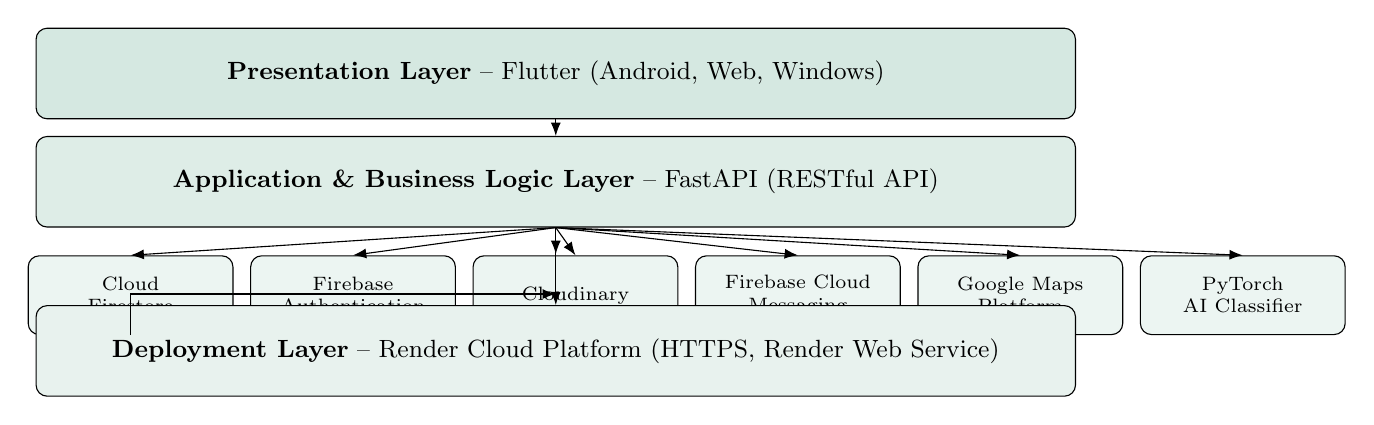
\begin{tikzpicture}[
      layer/.style={draw, rounded corners, minimum width=13.2cm, minimum height=1.15cm, align=center, font=\small},
      svc/.style={draw, rounded corners, fill=ecotracegreen!8, minimum width=2.6cm, minimum height=1cm, align=center, font=\scriptsize},
      node distance=6pt
    ]
    \node[layer, fill=ecotracegreen!18] (pres) {\textbf{Presentation Layer} -- Flutter (Android, Web, Windows)};
    \node[layer, below=of pres, fill=ecotracegreen!14] (app) {\textbf{Application \& Business Logic Layer} -- FastAPI (RESTful API)};
    \node[below=of app] (svcrow) {};
    \node[svc, below=10pt of app, xshift=-5.4cm] (db) {Cloud\\Firestore};
    \node[svc, right=6pt of db] (auth) {Firebase\\Authentication};
    \node[svc, right=6pt of auth] (media) {Cloudinary};
    \node[svc, right=6pt of media] (notif) {Firebase Cloud\\Messaging};
    \node[svc, right=6pt of notif] (maps) {Google Maps\\Platform};
    \node[svc, right=6pt of maps] (ai) {PyTorch\\AI Classifier};
    \node[layer, below=28pt of app, fill=ecotracegreen!10] (deploy) {\textbf{Deployment Layer} -- Render Cloud Platform (HTTPS, Render Web Service)};

    \draw[-Latex] (pres) -- (app);
    \draw[-Latex] (app.south) -- (svcrow.center);
    \foreach \s in {db,auth,media,notif,maps,ai} { \draw[-Latex] (app.south) -- (\s.north); }
    \draw[-Latex] (db.south) |- ($(deploy.north)+(0,4pt)$);
    \draw[-Latex] (app) -- (deploy);
  \end{tikzpicture}
  \caption{Overall System Architecture of EcoTrace, as proposed at the design stage. Source: Author's design.}
  \label{fig:system-architecture}
\end{figure}

\begin{table}[H]
\centering
\caption{Major Components of the EcoTrace System Architecture}
\label{tab:architecture-components}
\begin{tabular}{@{}p{2.6cm}p{3cm}p{7cm}@{}}
\toprule
\textbf{Architectural Layer} & \textbf{Technology} & \textbf{Primary Responsibility} \\
\midrule
Presentation Layer & Flutter (Android, Web, Windows) & Provides cross-platform user interfaces, navigation, forms, dashboards, maps, notifications, and role-specific interactions. \\
Application Layer & FastAPI & Processes requests, validates data, applies business rules, verifies authorization, coordinates integrations, and returns JSON responses. \\
Deployment Layer & Render & Hosts the FastAPI backend and provides HTTPS, environment variables, logging, health checks, and Git-based deployment. \\
Database Layer & Cloud Firestore & Stores user profiles, electronic waste records, workflows, notifications, reports, settings, and audit information. \\
Authentication Layer & Firebase Authentication & Provides account registration, login, password recovery, session management, and identity tokens. \\
Media Layer & Cloudinary & Stores, optimizes, transforms, and delivers electronic waste images. \\
Notification Layer & Firebase Cloud Messaging & Delivers targeted and system-wide push notifications. \\
Geospatial Layer & Google Maps Platform & Provides mapping, geocoding, location search, distance calculation, routing, and route optimization. \\
Artificial Intelligence Layer & PyTorch & Provides image preprocessing, electronic waste classification, and confidence-score generation. \\
\bottomrule
\end{tabular}
\end{table}

\subsection{Use Case Diagram and Actor Interactions}

A use case diagram represents the interactions between external actors and the
functions provided by a software system. It defines the system boundary,
identifies the categories of users, and shows the principal services available to
each actor.

The EcoTrace use case model contains ten main actors: (1)~Guest User;
(2)~Household User; (3)~Business User; (4)~Collector; (5)~Driver;
(6)~Technician; (7)~Recycler; (8)~Environmental Officer; (9)~Administrator;
and (10)~Super Administrator. Each actor performs different functions
according to assigned responsibilities and access permissions. Firebase
Authentication identifies registered users, while role-based access control
determines the functions that each actor can access.

\subsubsection{System Boundary}

The EcoTrace system boundary contains the major functions delivered
through the Android, Web, and Windows applications and the FastAPI backend.
External actors interact with the system through interfaces provided by the
presentation layer. The system processes requests, applies business rules,
communicates with external cloud services, stores records, and returns the
appropriate results.

The principal use case groups within the system boundary include
authentication and account management, electronic waste registration,
AI-assisted waste classification, pickup scheduling, collector and driver
assignment, collection and transportation, repair and refurbishment, recycling
and material recovery, marketplace management, notifications, environmental
monitoring, reporting and analytics, user and facility management, security
and audit management, and system configuration.

\subsubsection{Actor Interactions}

\textbf{Guest User.} The Guest User is an unauthenticated actor who accesses
public information and account-entry functions. The Guest User can view
public electronic waste awareness information, view publicly available
collection-centre information, register a new account, log in to an existing
account, and request password recovery. The Guest User must register and
authenticate before accessing protected EcoTrace functions.

\textbf{Household User.} The Household User represents an individual or
family that generates electronic waste. The Household User can manage a
personal profile, register electronic waste, upload waste images, request AI
classification, submit pickup requests, select a pickup location, track pickup
and collection status, receive notifications, view repair, refurbishment, and
recycling outcomes, browse marketplace listings, and view personal electronic
waste records.

\textbf{Business User.} The Business User represents an organization,
institution, company, or public office generating electronic waste. The
Business User can manage an organizational profile, register individual or
multiple electronic waste items, submit bulk collection requests, upload
images and supporting information, track organizational pickup requests,
monitor repair, recycling, and disposal outcomes, receive notifications, access
organizational reports, and maintain electronic waste disposal records.

\textbf{Collector.} The Collector is responsible for receiving and completing
pickup assignments. The Collector can view assigned pickup requests, accept
or reject assignments, view pickup locations and waste details, update
collection status, confirm item collection, upload collection evidence, report
collection exceptions, transfer collected waste to the next responsible actor,
and view completed collection history.

\textbf{Driver.} The Driver transports electronic waste between pickup
locations, collection centres, repair facilities, refurbishment facilities, and
recycling centres. The Driver can view assigned transportation tasks, access
pickup and destination locations, view suggested routes, follow optimized
routes where enabled, update departure, transit, arrival, and delivery status,
report delays or transportation incidents, record delivery details, and confirm
delivery to the receiving facility.

\textbf{Technician.} The Technician inspects, diagnoses, repairs, and
refurbishes electronic devices. The Technician can view assigned devices,
inspect and diagnose devices, determine repairability, record required parts
and estimated costs, update repair status, record replaced components,
perform functional testing, record refurbishment activities, assign quality
grades, approve devices for reuse or resale where authorized, and recommend
recycling for non-repairable devices.

\textbf{Recycler.} The Recycler processes electronic waste that cannot be
repaired or refurbished. The Recycler can view assigned recycling records,
receive and confirm electronic waste items, record dismantling activities,
record recovered components and materials, identify hazardous materials,
record residual waste, specify disposal methods, update recycling status,
confirm recycling completion, and generate recycling and material-recovery
reports.

\textbf{Environmental Officer.} The Environmental Officer monitors
electronic waste activities, environmental performance, and
compliance-related information. The Environmental Officer can view electronic
waste locations, monitor collection coverage, review transportation, repair,
refurbishment, and recycling activities, identify delayed or unresolved cases,
review material-recovery statistics, inspect facility records, record
environmental observations where implemented, view maps and analytical
dashboards, and generate environmental reports.

\textbf{Administrator.} The Administrator manages daily system operations
and coordinates the major EcoTrace workflows. The Administrator can manage
standard user accounts, verify operational users and organizations, manage
electronic waste categories, manage collection and processing facilities,
review pickup requests, assign collectors and drivers, monitor active
workflows, manage marketplace listings, publish announcements, review
operational reports, manage selected system content, and review permitted
audit records.

\textbf{Super Administrator.} The Super Administrator has the highest level
of system authority and manages high-risk administrative and security
operations. The Super Administrator can create and manage administrator
accounts, manage roles and permissions, configure system-wide settings,
review security and audit records, suspend or restore critical accounts, manage
integration configuration, review system health information, control
high-risk administrative functions, and monitor administrator activities.

\subsubsection{Major Use Case Relationships}

Some EcoTrace use cases depend on other use cases. These dependencies can
be represented using the \emph{include} relationship. Examples include:
Register Electronic Waste includes Validate Waste Information; Upload Waste
Image includes Validate Image File; Classify Electronic Waste includes
Preprocess Image; Submit Pickup Request includes Register Pickup Location;
Assign Collector includes Review Pickup Request; Complete Collection
includes Update Waste Lifecycle Status; Complete Repair includes Record
Repair Outcome; Complete Recycling includes Record Recovered Materials;
Generate Report includes Retrieve Authorized Data; and Perform Protected
Operation includes Verify Authentication and Role.

Optional or conditional behaviour may be represented using the
\emph{extend} relationship. Examples include: AI Classification extends
Register Electronic Waste; Upload Collection Evidence extends Complete
Collection; Report Transportation Incident extends Transport Electronic
Waste; Refurbish Device extends Repair Device; List Refurbished Item extends
Complete Refurbishment; and Send Status Notification extends major
workflow-status changes.

\subsubsection{Use Case Interaction Summary}

The use case model demonstrates that EcoTrace is a multi-actor system in
which each user category performs specialized functions. Household and
Business Users initiate the electronic waste lifecycle by registering items and
requesting collection. Collectors and Drivers coordinate collection and
transportation. Technicians determine whether devices can be repaired or
refurbished, while Recyclers process non-repairable waste and recover
materials. Environmental Officers monitor operational and environmental
performance. Administrators coordinate daily system activities, while Super
Administrators manage high-level security, permissions, and configuration.

The separation of actor responsibilities supports accountability, security,
workflow control, and complete electronic waste lifecycle traceability.
Figure~\ref{fig:use-case} presents the principal actors and use cases supported
by the EcoTrace system, and Table~\ref{tab:actor-summary} summarizes each
actor's principal use cases.

\begin{figure}[H]
  \centering
  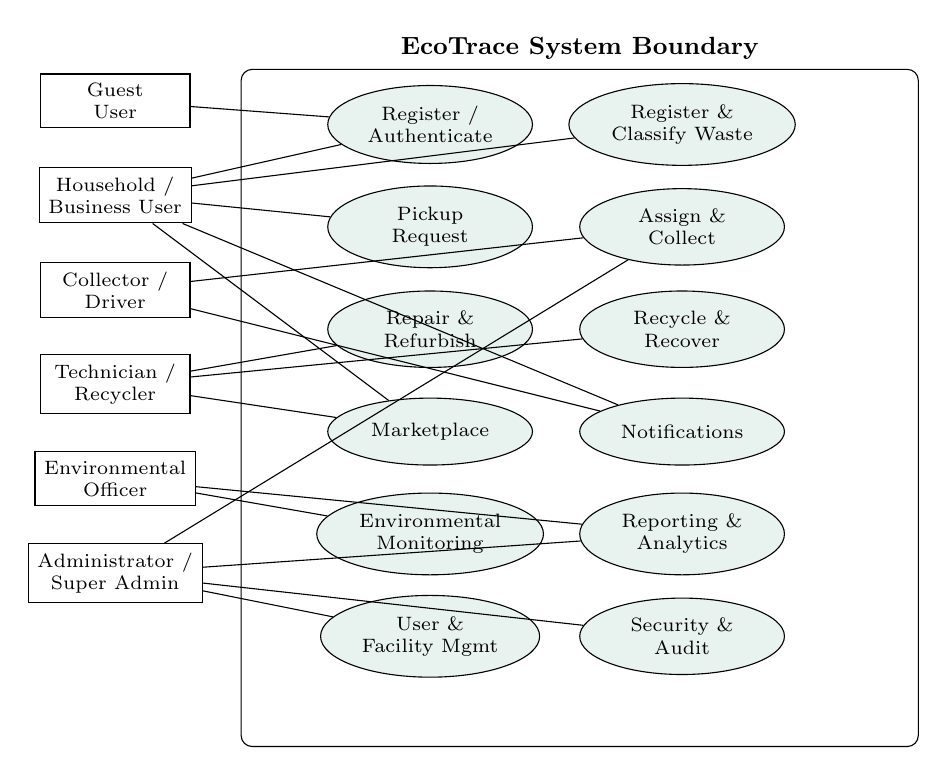
\begin{tikzpicture}[
      actor/.style={draw, align=center, font=\scriptsize, minimum width=1.9cm},
      uc/.style={draw, ellipse, align=center, font=\scriptsize, fill=ecotracegreen!10, minimum width=2.6cm, minimum height=0.85cm},
      boundary/.style={draw, rounded corners, minimum width=8.6cm, minimum height=8.6cm}
    ]
    \node[boundary, label={[font=\small\bfseries]above:EcoTrace System Boundary}] (b) at (4.3,-4.3) {};
    \node[actor] (guest) at (-1.6,-0.4) {Guest\\User};
    \node[actor] (hh) at (-1.6,-1.6) {Household /\\Business User};
    \node[actor] (coll) at (-1.6,-2.8) {Collector /\\Driver};
    \node[actor] (tech) at (-1.6,-4.0) {Technician /\\Recycler};
    \node[actor] (env) at (-1.6,-5.2) {Environmental\\Officer};
    \node[actor] (admin) at (-1.6,-6.4) {Administrator /\\Super Admin};

    \node[uc] (auth) at (2.4,-0.7) {Register /\\Authenticate};
    \node[uc] (reg) at (5.6,-0.7) {Register \&\\Classify Waste};
    \node[uc] (pick) at (2.4,-2.0) {Pickup\\Request};
    \node[uc] (asgn) at (5.6,-2.0) {Assign \&\\Collect};
    \node[uc] (repr) at (2.4,-3.3) {Repair \&\\Refurbish};
    \node[uc] (recy) at (5.6,-3.3) {Recycle \&\\Recover};
    \node[uc] (mkt) at (2.4,-4.6) {Marketplace};
    \node[uc] (not) at (5.6,-4.6) {Notifications};
    \node[uc] (env2) at (2.4,-5.9) {Environmental\\Monitoring};
    \node[uc] (rpt) at (5.6,-5.9) {Reporting \&\\Analytics};
    \node[uc] (adm2) at (2.4,-7.2) {User \&\\Facility Mgmt};
    \node[uc] (sec) at (5.6,-7.2) {Security \&\\Audit};

    \draw (guest) -- (auth);
    \draw (hh) -- (auth); \draw (hh) -- (reg); \draw (hh) -- (pick); \draw (hh) -- (mkt); \draw (hh) -- (not);
    \draw (coll) -- (asgn); \draw (coll) -- (not);
    \draw (tech) -- (repr); \draw (tech) -- (recy); \draw (tech) -- (mkt);
    \draw (env) -- (env2); \draw (env) -- (rpt);
    \draw (admin) -- (adm2); \draw (admin) -- (sec); \draw (admin) -- (rpt); \draw (admin) -- (asgn);
  \end{tikzpicture}
  \caption{Overall Use Case Diagram for EcoTrace. Source: Author's design.}
  \label{fig:use-case}
\end{figure}

\begin{table}[H]
\centering
\small
\caption{Summary of EcoTrace Actors and Principal Use Cases}
\label{tab:actor-summary}
\begin{tabular}{@{}p{3.2cm}p{9.4cm}@{}}
\toprule
\textbf{Actor} & \textbf{Principal Use Cases} \\
\midrule
Guest User & View public information, register an account, log in, and request password recovery. \\
Household User & Register electronic waste, upload images, request AI classification, schedule pickups, track status, receive notifications, and browse the marketplace. \\
Business User & Manage organizational waste records, submit bulk pickup requests, monitor recovery outcomes, and generate organizational reports. \\
Collector & View assignments, accept pickup tasks, collect waste, upload evidence, update statuses, and complete collections. \\
Driver & View transport assignments, access routes, update transport status, report incidents, and confirm delivery. \\
Technician & Inspect devices, diagnose faults, repair devices, refurbish devices, record test results, and recommend recycling. \\
Recycler & Receive waste, dismantle devices, record recovered materials, identify hazardous waste, complete recycling, and generate recovery records. \\
Environmental Officer & Monitor activities, inspect maps and reports, review recovery performance, identify unresolved cases, and generate environmental reports. \\
Administrator & Manage users, categories, facilities, requests, assignments, marketplace listings, announcements, and operational reports. \\
Super Administrator & Manage administrators, roles, permissions, security, audit logs, integrations, and system-wide configuration. \\
\bottomrule
\end{tabular}
\end{table}

\textit{Note: the actor-to-use-case mapping in Table~\ref{tab:actor-summary} was
reconstructed from the source document's own actor descriptions, since the
original table's layout did not survive text extraction from the source PDF
cleanly. The use-case content itself is unchanged.}

\subsection{Data Flow Diagram}

A Data Flow Diagram (DFD) illustrates how information moves between
external entities, system processes, data stores, and outputs. It describes the
logical movement and transformation of data without specifying the
programming code or physical implementation used to perform each
operation. The EcoTrace data flow model is presented at two levels: the
Context-Level DFD, which represents EcoTrace as one complete process and
shows its interactions with external entities; and the Level-One DFD, which
decomposes the complete system into its principal operational processes and
data stores.

\subsubsection{Context-Level Data Flow Diagram}

The context-level DFD represents the complete EcoTrace system as a single
process identified as Process 0. It defines the system boundary and shows the
principal information exchanged between EcoTrace and its external users and
services. To maintain readability, actors with closely related responsibilities
are grouped within the context diagram; their detailed responsibilities are
expanded in the Level-One DFD and the use case model.

The principal external entities are: (1)~Guest and Public User;
(2)~Household and Business User; (3)~Collector and Driver; (4)~Technician
and Recycler; (5)~Environmental Officer; (6)~Administrator and Super
Administrator; and (7)~External Cloud and Artificial Intelligence Services
(Firebase Authentication, Cloud Firestore, Cloudinary, Firebase Cloud
Messaging, Google Maps Platform, PyTorch, and Render).
Figure~\ref{fig:context-dfd} presents the principal information flows between
EcoTrace, its users, and the external cloud services supporting the system, and
Table~\ref{tab:context-dfd} summarizes the data exchanged with each entity.

\begin{figure}[H]
  \centering
  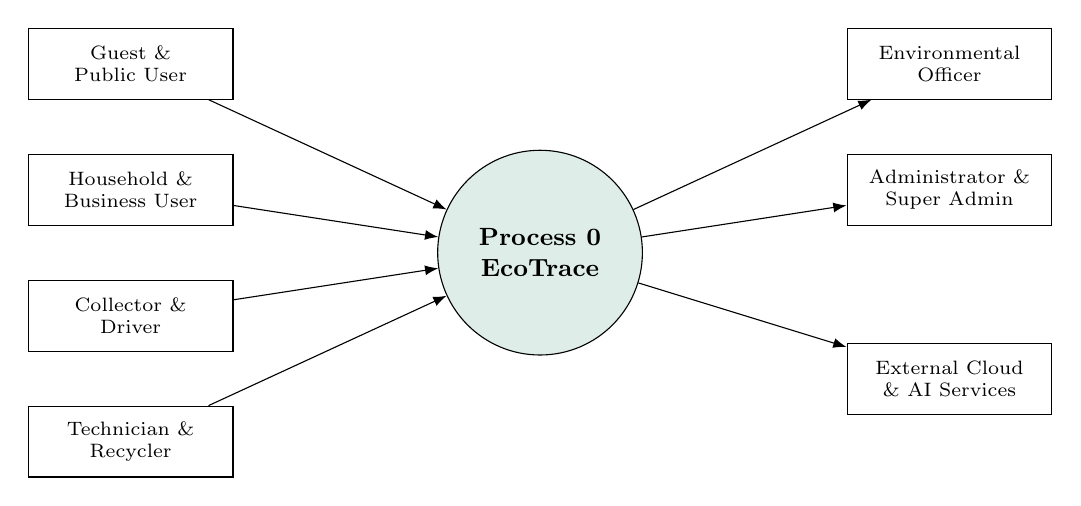
\begin{tikzpicture}[
      ent/.style={draw, align=center, font=\scriptsize, minimum width=2.6cm, minimum height=0.9cm},
      proc/.style={draw, circle, align=center, font=\small\bfseries, fill=ecotracegreen!14, minimum size=2.6cm},
      arr/.style={-Latex, font=\tiny}
    ]
    \node[proc] (p0) at (0,0) {Process 0\\EcoTrace};
    \node[ent] (a) at (-5.2,2.4) {Guest \&\\Public User};
    \node[ent] (b) at (-5.2,0.8) {Household \&\\Business User};
    \node[ent] (c) at (-5.2,-0.8) {Collector \&\\Driver};
    \node[ent] (d) at (-5.2,-2.4) {Technician \&\\Recycler};
    \node[ent] (e) at (5.2,2.4) {Environmental\\Officer};
    \node[ent] (f) at (5.2,0.8) {Administrator \&\\Super Admin};
    \node[ent] (g) at (5.2,-1.6) {External Cloud\\\& AI Services};
    \draw[arr] (a) -- (p0); \draw[arr] (b) -- (p0); \draw[arr] (c) -- (p0); \draw[arr] (d) -- (p0);
    \draw[arr] (p0) -- (e); \draw[arr] (p0) -- (f); \draw[arr] (p0) -- (g);
  \end{tikzpicture}
  \caption{Context-Level Data Flow Diagram of the EcoTrace System. Source: Author's design.}
  \label{fig:context-dfd}
\end{figure}

\begin{longtable}{@{}p{3.1cm}p{5cm}p{5.3cm}@{}}
\caption{External Entities and Data Flows in the EcoTrace Context Diagram} \label{tab:context-dfd} \\
\toprule \textbf{External Entity} & \textbf{Data Sent to EcoTrace} & \textbf{Data Received from EcoTrace} \\ \midrule
\endfirsthead
\toprule \textbf{External Entity} & \textbf{Data Sent to EcoTrace} & \textbf{Data Received from EcoTrace} \\ \midrule
\endhead
Guest and Public User & Registration data, login credentials, password-recovery requests, public-information requests. & Public information, registration confirmation, authentication results, recovery instructions. \\
Household and Business User & Profile data, electronic waste records, images, pickup requests, locations, marketplace enquiries, report requests. & Classification results, pickup status, collection updates, recovery outcomes, notifications, marketplace information, reports. \\
Collector and Driver & Task responses, collection updates, transport updates, evidence, delivery confirmations, incident reports. & Assignments, waste details, schedules, pickup locations, destinations, route information. \\
Technician and Recycler & Inspection findings, repair records, refurbishment records, recycling records, material-recovery information. & Assigned items, device details, lifecycle history, processing instructions. \\
Environmental Officer & Monitoring requests, report filters, inspection observations, compliance findings. & Maps, environmental reports, alerts, recovery statistics, facility records, analytical dashboards. \\
Administrator and Super Administrator & User-management actions, assignments, role changes, facility data, announcements, report requests, configuration changes. & Administrative dashboards, user and account records, workflow status, assignment results, system reports, audit logs, security alerts, configuration status. \\
External Cloud and AI Services & Authentication requests, database operations, media files, notification requests, geographic requests, images for AI classification. & Authentication tokens, stored data, image URLs, delivery results, routes, location information, prediction results. \\
\bottomrule
\end{longtable}

\subsubsection{Level-One Data Flow Diagram}

The Level-One DFD expands Process 0 into its major internal processes,
data stores, and information flows. It provides a more detailed logical view of
how data moves through the system during registration, collection, logistics,
recovery, reporting, and administration. The system is decomposed into eight
major processes, each reading from and writing to its own principal data
store: 1.0~Manage Authentication and User Accounts (D1); 2.0~Manage
Electronic Waste Registration and AI Classification (D2); 3.0~Manage Pickup
Requests and Assignments (D3); 4.0~Manage Collection, Transportation, and
Routing (D4); 5.0~Manage Repair, Refurbishment, and Recycling (D5);
6.0~Manage Marketplace and Notifications (D6); 7.0~Manage Reporting and
Environmental Monitoring (D7); and 8.0~Manage Administration, Security,
and Configuration (D8).

\begin{itemize}
  \item \textbf{Process 1.0} handles registration, login, password recovery, and
    profile management. It communicates with Firebase Authentication for
    identity verification and reads/writes D1~--~User Accounts and Profiles.
  \item \textbf{Process 2.0} manages waste registration, image upload, and
    AI-based classification. It writes to D2~--~Electronic Waste Records,
    uploads images through Cloudinary, and communicates with the PyTorch
    classification service.
  \item \textbf{Process 3.0} handles pickup scheduling, validation, review, and
    collector/driver assignment. It reads D2 and writes D3~--~Pickup and
    Assignment Records.
  \item \textbf{Process 4.0} manages collection execution, transport, route
    display, and delivery confirmation. It communicates with Google Maps
    Platform and writes D4~--~Transportation and Route Records, updating D3.
  \item \textbf{Process 5.0} manages inspection, repair, refurbishment,
    recycling, and material recovery. It reads D2 and writes D5~--~Repair,
    Refurbishment, and Recycling Records.
  \item \textbf{Process 6.0} manages marketplace listings and notification
    delivery. It writes D6~--~Marketplace and Notification Records and
    communicates with Firebase Cloud Messaging.
  \item \textbf{Process 7.0} generates dashboards, reports, and monitoring
    views. It reads D2--D6 and writes D7~--~Reports, Monitoring, and Audit
    Records.
  \item \textbf{Process 8.0} manages user administration, roles, facilities,
    audit review, and configuration. It updates D1, D7, and D8~--~Configuration
    and Reference Data.
\end{itemize}

This decomposition shows that authentication, waste registration, pickup
management, logistics, recovery operations, reporting, monitoring, and
administration are handled through distinct but interconnected processes, and
that Cloud Firestore-based records, media services, notification services,
geospatial services, and AI services are integrated into the logical operation of
the system. Figure~\ref{fig:level1-dfd} illustrates the major internal processes,
data stores, and data flows, and Table~\ref{tab:level1-dfd} summarizes each
process.

\begin{figure}[H]
  \centering
  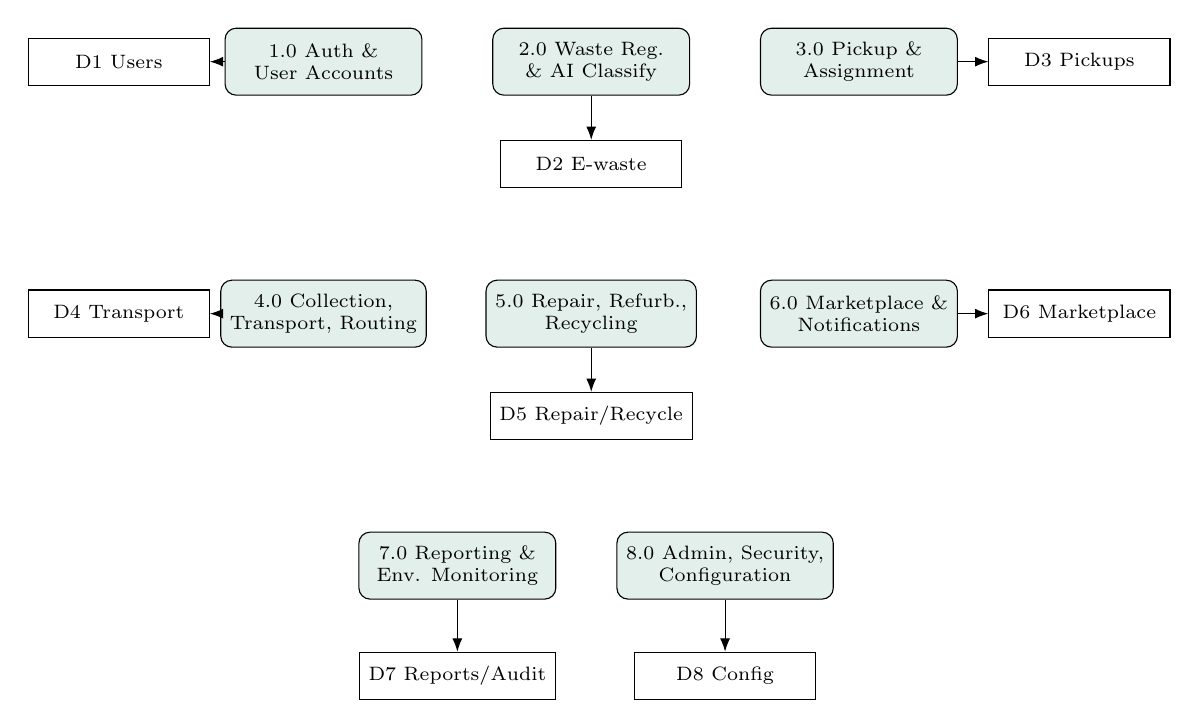
\begin{tikzpicture}[
      proc/.style={draw, rounded corners, align=center, font=\scriptsize, fill=ecotracegreen!12, minimum width=2.5cm, minimum height=0.85cm},
      store/.style={draw, minimum width=2.3cm, minimum height=0.6cm, font=\scriptsize, align=center},
      arr/.style={-Latex, font=\tiny}
    ]
    \node[proc] (p1) at (0,3.2)   {1.0 Auth \&\\User Accounts};
    \node[proc] (p2) at (3.4,3.2) {2.0 Waste Reg.\\\& AI Classify};
    \node[proc] (p3) at (6.8,3.2) {3.0 Pickup \&\\Assignment};
    \node[proc] (p4) at (0,0)     {4.0 Collection,\\Transport, Routing};
    \node[proc] (p5) at (3.4,0)   {5.0 Repair, Refurb.,\\Recycling};
    \node[proc] (p6) at (6.8,0)   {6.0 Marketplace \&\\Notifications};
    \node[proc] (p7) at (1.7,-3.2) {7.0 Reporting \&\\Env. Monitoring};
    \node[proc] (p8) at (5.1,-3.2) {8.0 Admin, Security,\\Configuration};
    \node[store] (d1) at (-2.6,3.2) {D1 Users};
    \node[store] (d2) at (3.4,1.9) {D2 E-waste};
    \node[store] (d3) at (9.6,3.2) {D3 Pickups};
    \node[store] (d4) at (-2.6,0) {D4 Transport};
    \node[store] (d5) at (3.4,-1.3) {D5 Repair/Recycle};
    \node[store] (d6) at (9.6,0) {D6 Marketplace};
    \node[store] (d7) at (1.7,-4.6) {D7 Reports/Audit};
    \node[store] (d8) at (5.1,-4.6) {D8 Config};
    \foreach \p/\d in {p1/d1,p2/d2,p3/d3,p4/d4,p5/d5,p6/d6,p7/d7,p8/d8} { \draw[arr] (\p) -- (\d); }
  \end{tikzpicture}
  \caption{Level-One Data Flow Diagram of the EcoTrace System. Source: Author's design.}
  \label{fig:level1-dfd}
\end{figure}

\begin{longtable}{@{}p{1.4cm}p{4.4cm}p{6.6cm}@{}}
\caption{Major Processes in the EcoTrace Level-One Data Flow Diagram} \label{tab:level1-dfd} \\
\toprule \textbf{Process} & \textbf{Process Name} & \textbf{Primary Function} \\ \midrule
\endfirsthead
\toprule \textbf{Process} & \textbf{Process Name} & \textbf{Primary Function} \\ \midrule
\endhead
1.0 & Manage Authentication and User Accounts & Handles registration, login, password recovery, profile management, role retrieval, and access verification. \\
2.0 & Manage Electronic Waste Registration and AI Classification & Handles waste registration, image upload, item storage, and AI-based classification of electronic waste images. \\
3.0 & Manage Pickup Requests and Assignments & Handles pickup scheduling, request validation, review, and assignment of collectors and drivers. \\
4.0 & Manage Collection, Transportation, and Routing & Handles collection operations, transportation tracking, route display, delivery updates, and related logistics. \\
5.0 & Manage Repair, Refurbishment, and Recycling & Handles inspection, diagnosis, repair, refurbishment, recycling, and material-recovery activities. \\
6.0 & Manage Marketplace and Notifications & Handles marketplace listings, browsing, announcements, and push notifications. \\
7.0 & Manage Reporting and Environmental Monitoring & Handles dashboards, analytical views, reports, environmental monitoring, and related queries. \\
8.0 & Manage Administration, Security, and Configuration & Handles user administration, roles, facilities, audit review, security oversight, and system settings. \\
\bottomrule
\end{longtable}

\subsection{Sequence Diagrams}

A sequence diagram shows how actors and system components interact over
time to complete a specific operation. It emphasizes the order of messages
exchanged between the user interface, backend services, databases, and
external platforms. The principal EcoTrace sequence diagrams cover user
authentication, electronic waste registration and image upload, AI-based
classification, pickup request and assignment, collection and transportation,
repair/refurbishment/recycling, and report generation and environmental
monitoring.

\subsubsection{User Authentication Sequence}
The sequence proceeds as follows: (1)~the user enters an email address and
password; (2)~the Flutter application validates the required fields; (3)~the
application submits the credentials to Firebase Authentication; (4)~Firebase
Authentication verifies the credentials; (5)~if valid, Firebase returns an
authentication token; (6)~the Flutter application sends the token to the
FastAPI backend; (7)~FastAPI verifies the token and retrieves the user's
profile and role from Cloud Firestore; (8)~Cloud Firestore returns the profile
and role information; (9)~FastAPI returns an authorized session response; and
(10)~the Flutter application redirects the user to the appropriate role-based
dashboard. If authentication fails, Firebase Authentication returns an error
and the Flutter application displays an appropriate message.

\begin{figure}[H]
  \centering
  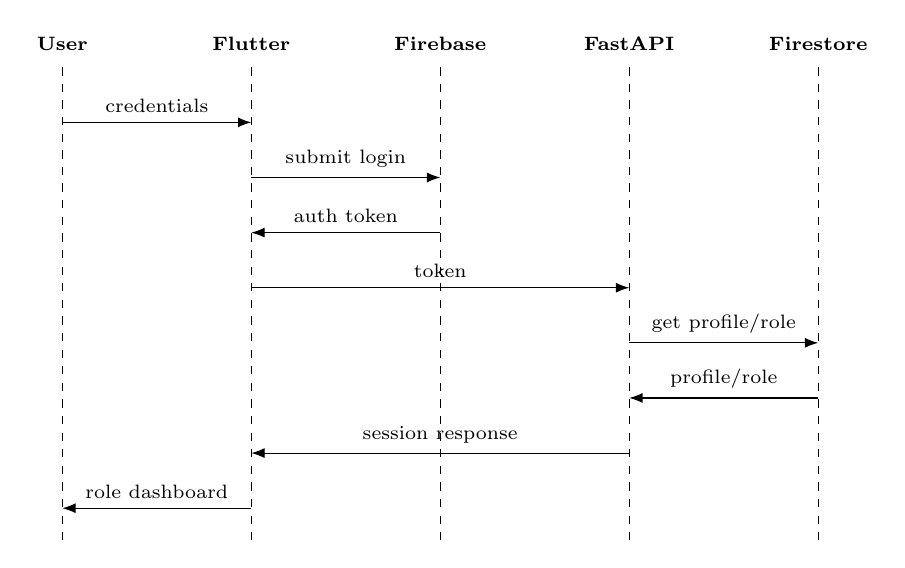
\begin{tikzpicture}[font=\scriptsize]
    \foreach \name/\x in {User/0,Flutter/2.4,Firebase/4.8,FastAPI/7.2,Firestore/9.6} {
      \node at (\x,0) {\textbf{\name}};
      \draw[dashed] (\x,-0.3) -- (\x,-6.3);
    }
    \draw[-Latex] (0,-1) -- (2.4,-1) node[midway,above]{credentials};
    \draw[-Latex] (2.4,-1.7) -- (4.8,-1.7) node[midway,above]{submit login};
    \draw[-Latex] (4.8,-2.4) -- (2.4,-2.4) node[midway,above]{auth token};
    \draw[-Latex] (2.4,-3.1) -- (7.2,-3.1) node[midway,above]{token};
    \draw[-Latex] (7.2,-3.8) -- (9.6,-3.8) node[midway,above]{get profile/role};
    \draw[-Latex] (9.6,-4.5) -- (7.2,-4.5) node[midway,above]{profile/role};
    \draw[-Latex] (7.2,-5.2) -- (2.4,-5.2) node[midway,above]{session response};
    \draw[-Latex] (2.4,-5.9) -- (0,-5.9) node[midway,above]{role dashboard};
  \end{tikzpicture}
  \caption{Authentication Sequence Diagram for EcoTrace. Source: Author's design.}
  \label{fig:seq-auth}
\end{figure}

\subsubsection{Electronic Waste Registration and Image Upload Sequence}
(1)~The user opens the electronic waste registration form; (2)~the Flutter
application displays the required fields; (3)~the user enters waste details and
selects an image; (4)~the Flutter application validates the basic input; (5)~the
application sends the image and registration data to the FastAPI backend;
(6)~FastAPI verifies the user's authentication token and role; (7)~FastAPI
validates the submitted data and image file; (8)~FastAPI uploads the image to
Cloudinary; (9)~Cloudinary stores the image and returns a secure image URL;
(10)~FastAPI creates the electronic waste record in Cloud Firestore, including
the image URL and lifecycle status; (11)~Cloud Firestore returns the created
record identifier; (12)~FastAPI returns a successful registration response; and
(13)~the Flutter application displays the registered item and confirmation
message.

\subsubsection{AI Classification Sequence}
(1)~The user selects the AI classification function; (2)~the Flutter
application sends the image or image reference to the FastAPI backend;
(3)~FastAPI verifies the user's authentication and authorization; (4)~FastAPI
retrieves or receives the image; (5)~the backend validates and preprocesses the
image; (6)~the preprocessed image is passed to the trained PyTorch model;
(7)~the PyTorch model performs inference; (8)~the model returns the
predicted waste category and confidence score; (9)~FastAPI formats the
result; (10)~the result is stored with the relevant waste record in Cloud
Firestore where appropriate; (11)~FastAPI returns the classification result to
the Flutter application; (12)~the Flutter application displays the predicted
category and confidence score; and (13)~the user may accept or correct the
result.

\subsubsection{Pickup Request and Assignment Sequence}
(1)~The user selects one or more registered electronic waste items; (2)~the
user enters a preferred pickup date, location, and collection instructions;
(3)~the Flutter application sends the pickup request to FastAPI; (4)~FastAPI
validates the request and user ownership; (5)~FastAPI stores the request in
Cloud Firestore; (6)~Cloud Firestore returns the request identifier; (7)~FastAPI
sends a notification request through Firebase Cloud Messaging; (8)~the
administrator receives a new-request notification; (9)~the administrator opens
the request and reviews its details; (10)~the administrator selects a collector
and driver; (11)~the Flutter administrative interface sends the assignment to
FastAPI; (12)~FastAPI validates the selected operational users; (13)~FastAPI
updates the pickup and assignment records in Cloud Firestore; (14)~FastAPI
sends assignment notifications through Firebase Cloud Messaging; and
(15)~the household or business user, collector, and driver receive updated
status information.
\begin{figure}[H]
  \centering
  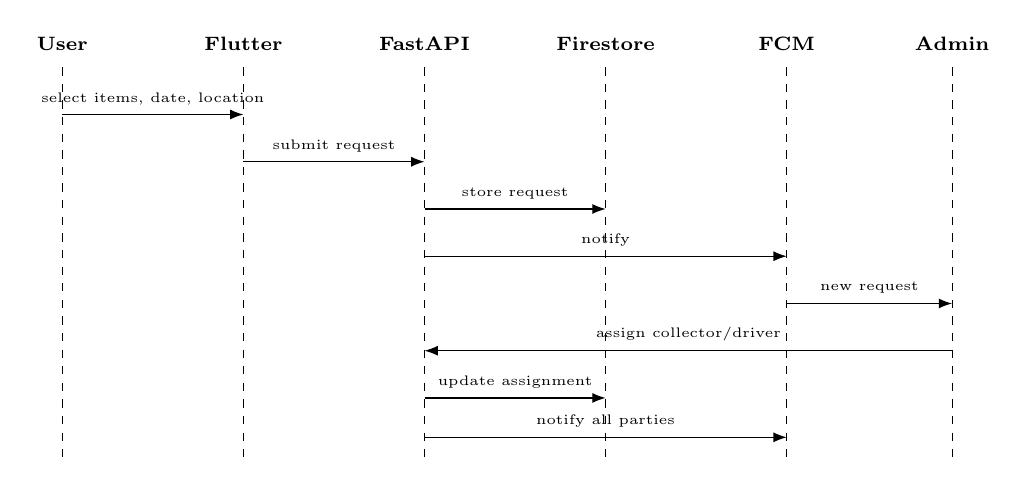
\begin{tikzpicture}[font=\scriptsize]
    \foreach \name/\x in {User/0,Flutter/2.3,FastAPI/4.6,Firestore/6.9,FCM/9.2,Admin/11.3} {
      \node at (\x,0) {\textbf{\name}};
      \draw[dashed] (\x,-0.3) -- (\x,-5.3);
    }
    \draw[-Latex] (0,-0.9) -- (2.3,-0.9) node[midway,above,font=\tiny]{select items, date, location};
    \draw[-Latex] (2.3,-1.5) -- (4.6,-1.5) node[midway,above,font=\tiny]{submit request};
    \draw[-Latex] (4.6,-2.1) -- (6.9,-2.1) node[midway,above,font=\tiny]{store request};
    \draw[-Latex] (4.6,-2.7) -- (9.2,-2.7) node[midway,above,font=\tiny]{notify};
    \draw[-Latex] (9.2,-3.3) -- (11.3,-3.3) node[midway,above,font=\tiny]{new request};
    \draw[-Latex] (11.3,-3.9) -- (4.6,-3.9) node[midway,above,font=\tiny]{assign collector/driver};
    \draw[-Latex] (4.6,-4.5) -- (6.9,-4.5) node[midway,above,font=\tiny]{update assignment};
    \draw[-Latex] (4.6,-5.0) -- (9.2,-5.0) node[midway,above,font=\tiny]{notify all parties};
  \end{tikzpicture}
  \caption{Pickup, Assignment, Collection, and Transportation Sequence Diagram. Source: Author's design.}
  \label{fig:seq-pickup}
\end{figure}

\subsubsection{Collection and Transportation Sequence}
(1)~The collector opens the assigned pickup task; (2)~the Flutter application
requests the pickup details from FastAPI; (3)~FastAPI retrieves the request
and location information from Cloud Firestore; (4)~FastAPI requests route
information from Google Maps Platform where required; (5)~Google Maps
Platform returns distance, route, and estimated travel information; (6)~FastAPI
returns the task and route details to the collector or driver; (7)~the collector
accepts the task and updates the status; (8)~FastAPI stores the updated status
in Cloud Firestore; (9)~the collector reaches the pickup location and confirms
collection; (10)~the collector uploads evidence where required; (11)~FastAPI
stores the collection record and updates the waste lifecycle status; (12)~the
driver transports the waste to the assigned destination; (13)~the driver
updates transit and delivery status; (14)~FastAPI stores the transportation
record; (15)~the receiving facility confirms delivery; and (16)~Firebase Cloud
Messaging sends status notifications to the relevant users.

\subsubsection{Repair, Refurbishment, and Recycling Sequence}
(1)~The technician or recycler opens the assigned item; (2)~the Flutter
application requests the item and lifecycle history; (3)~FastAPI retrieves the
item, collection, and transport records from Cloud Firestore; (4)~the
technician inspects the device and records findings; (5)~FastAPI stores the
inspection record; (6)~if the item is repairable, the technician records repair
or refurbishment activities; (7)~FastAPI updates the relevant records in Cloud
Firestore; (8)~if the item is not repairable, it is assigned to the recycler;
(9)~the recycler records dismantling, recovered materials, hazardous
materials, and residual waste; (10)~FastAPI stores the recycling record and
updates the waste lifecycle status; (11)~where applicable, an approved
refurbished item is added to the marketplace; (12)~Firebase Cloud Messaging
sends completion or status notifications; and (13)~relevant users can view the
final recovery outcome.
\begin{figure}[H]
  \centering
  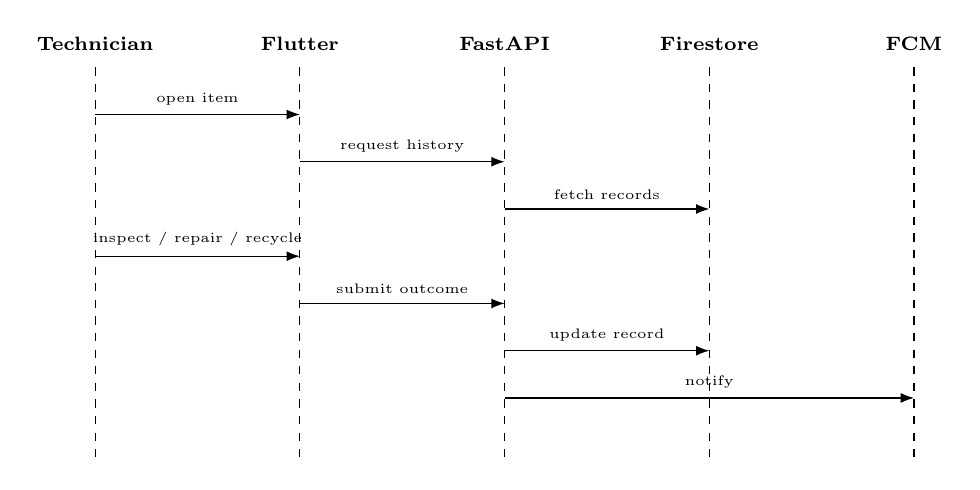
\begin{tikzpicture}[font=\scriptsize]
    \foreach \name/\x in {Technician/0,Flutter/2.6,FastAPI/5.2,Firestore/7.8,FCM/10.4} {
      \node at (\x,0) {\textbf{\name}};
      \draw[dashed] (\x,-0.3) -- (\x,-5.3);
    }
    \draw[-Latex] (0,-0.9) -- (2.6,-0.9) node[midway,above,font=\tiny]{open item};
    \draw[-Latex] (2.6,-1.5) -- (5.2,-1.5) node[midway,above,font=\tiny]{request history};
    \draw[-Latex] (5.2,-2.1) -- (7.8,-2.1) node[midway,above,font=\tiny]{fetch records};
    \draw[-Latex] (0,-2.7) -- (2.6,-2.7) node[midway,above,font=\tiny]{inspect / repair / recycle};
    \draw[-Latex] (2.6,-3.3) -- (5.2,-3.3) node[midway,above,font=\tiny]{submit outcome};
    \draw[-Latex] (5.2,-3.9) -- (7.8,-3.9) node[midway,above,font=\tiny]{update record};
    \draw[-Latex] (5.2,-4.5) -- (10.4,-4.5) node[midway,above,font=\tiny]{notify};
  \end{tikzpicture}
  \caption{Repair, Refurbishment, Recycling, and Reporting Sequence Diagram. Source: Author's design.}
  \label{fig:seq-repair}
\end{figure}

\subsubsection{Report Generation and Environmental Monitoring Sequence}
(1)~The authorized user opens the reporting dashboard; (2)~the user selects
report type, date range, status, category, location, or other filters; (3)~the
Flutter application sends the report request to FastAPI; (4)~FastAPI verifies
the user's role and report permissions; (5)~FastAPI retrieves relevant data
from Cloud Firestore; (6)~FastAPI aggregates and analyses the retrieved
records; (7)~FastAPI may request map or location information from Google
Maps Platform; (8)~FastAPI prepares the report data; (9)~the report is
returned to the Flutter application; (10)~the application displays tables,
charts, maps, and summary indicators; (11)~the authorized user may export
the report in PDF or another supported format; and (12)~the report request or
export action may be recorded in the audit log.

\subsubsection{Sequence Diagram Summary}
The sequence diagrams demonstrate how EcoTrace coordinates user actions,
Flutter applications, FastAPI services, Cloud Firestore, Firebase, Cloudinary,
Google Maps Platform, and PyTorch. They also show that authentication,
validation, authorization, cloud storage, notification delivery, route services,
and AI inference occur through ordered interactions rather than isolated
system operations.

\subsection{Database Design and Cloud Firestore Collections}

Database design defines how application data is structured, stored, related,
retrieved, updated, secured, and maintained. EcoTrace uses Cloud Firestore as
its primary database because it supports flexible document-based data
storage, real-time synchronization, cloud accessibility, security rules, and
integration with Firebase Authentication.

Cloud Firestore is a NoSQL document database. Instead of storing data in
relational tables, it organizes information into collections and documents. A
collection contains related documents, while each document contains fields
represented as key-value pairs. The EcoTrace database design separates
information according to the major system modules. This modular structure
improves maintainability, security, query performance, and future scalability.

The principal collections proposed for EcoTrace are: users, roles,
ewaste\_records, pickup\_requests, assignments, transportation\_records,
collection\_centres, facilities, repair\_records, refurbishment\_records,
recycling\_records, recovered\_materials, marketplace\_listings, notifications,
environmental\_reports, audit\_logs, system\_settings, and reference\_data.

\subsubsection{Collection Descriptions}

\textbf{users.} Stores profile and authorization-related information for
registered users. Firebase Authentication manages the user's email, password
credentials, authentication token, and authentication identifier, while Cloud
Firestore stores additional application-specific profile information. A typical
document may contain: userId, firebaseUid, fullName, email, phoneNumber,
roleId, organizationName, profileImageUrl, address, district, latitude,
longitude, accountStatus, isVerified, createdAt, updatedAt, and lastLoginAt.
The document identifier may use the Firebase Authentication user identifier
to simplify user-profile retrieval.

\textbf{roles.} Stores the available system roles and their associated
permissions: roleId, roleName, description, permissions, isActive, createdAt,
updatedAt. Examples of role values include household, business, collector,
driver, technician, recycler, environmental officer, administrator, and super
administrator.

\textbf{ewaste\_records.} Stores the main information associated with
registered electronic waste items: ewasteId, ownerId, ownerType, categoryId,
deviceName, brand, model, serialNumber, quantity, condition, description,
imageUrls, aiPredictedCategory, aiConfidenceScore, classificationSource,
latitude, longitude, address, preferredRecoveryOption, lifecycleStatus,
createdAt, updatedAt. The lifecycleStatus field may contain values such as
registered, pickup requested, assigned, collected, transported, under
inspection, under repair, refurbished, recycled, listed, reused, or disposed.

\textbf{pickup\_requests.} Stores requests submitted by household and
business users: pickupRequestId, requesterId, ewasteIds, pickupAddress,
latitude, longitude, preferredDate, preferredTime, contactName, contactPhone,
collectionInstructions, status, rejectionReason, cancellationReason,
submittedAt, scheduledAt, completedAt, updatedAt.

\textbf{assignments.} Stores the assignment of collectors, drivers,
technicians, and recyclers to operational records: assignmentId,
referenceType, referenceId, assignedUserId, assignedRole, assignedBy,
assignmentStatus, acceptedAt, rejectedAt, rejectionReason, assignedAt,
updatedAt. The referenceType field identifies whether the assignment relates
to pickup, transportation, repair, refurbishment, or recycling.

\textbf{transportation\_records.} Stores the movement of electronic waste
between operational locations: transportId, pickupRequestId, driverId,
vehicleId, originAddress, originLatitude, originLongitude, destinationAddress,
destinationLatitude, destinationLongitude, routeDistance, estimatedDuration,
routePolyline, status, incidentDescription, departedAt, arrivedAt, deliveredAt,
updatedAt.

\textbf{collection\_centres.} Stores approved electronic waste collection
locations: centreId, centreName, centreType, address, district, latitude,
longitude, contactPhone, email, operatingHours, acceptedWasteCategories,
verificationStatus, isActive, createdAt, updatedAt.

\textbf{facilities.} Stores repair centres, refurbishment centres, recycling
facilities, warehouses, and other processing locations: facilityId,
facilityName, facilityType, operatorId, address, latitude, longitude,
contactInformation, supportedOperations, capacity, verificationStatus,
isActive, createdAt, updatedAt.

\textbf{repair\_records.} Stores inspection, diagnosis, repair planning, and
repair-outcome information: repairId, ewasteId, technicianId, facilityId,
inspectionFindings, diagnosis, isRepairable, requiredParts, estimatedCost,
actualCost, replacedComponents, repairStatus, testResults, finalOutcome,
startedAt, completedAt, updatedAt.

\textbf{refurbishment\_records.} Stores information about devices restored
for reuse or resale: refurbishmentId, ewasteId, technicianId, facilityId,
activitiesPerformed, componentsReplaced, softwareUpdated,
functionalTestResults, cosmeticCondition, qualityGrade, approvalStatus,
approvedBy, finalCondition, startedAt, completedAt, updatedAt.

\textbf{recycling\_records.} Stores dismantling, processing,
material-recovery, and final-disposal information: recyclingId, ewasteId,
recyclerId, facilityId, quantityReceived, receivedCondition,
dismantlingActivities, hazardousMaterials, residualWaste, disposalMethod,
recyclingStatus, receivedAt, completedAt, updatedAt.

\textbf{recovered\_materials.} Stores materials and components recovered
during recycling: materialRecordId, recyclingId, materialType, materialName,
quantity, unit, qualityCondition, estimatedValue, destination,
marketplaceEligible, recordedBy, recordedAt.

\textbf{marketplace\_listings.} Stores refurbished devices, reusable
components, and recovered materials offered through the marketplace:
listingId, sourceRecordType, sourceRecordId, sellerId, title, description,
category, condition, qualityGrade, price, currency, quantityAvailable,
imageUrls, listingStatus, approvalStatus, approvedBy, createdAt, updatedAt.

\textbf{notifications.} Stores in-application notification records:
notificationId, recipientId, recipientRole, title, message, notificationType,
referenceType, referenceId, isRead, deliveryStatus, createdAt, readAt.

\textbf{environmental\_reports.} Stores submitted observations, inspection
findings, environmental assessments, and generated report metadata:
reportId, reportType, generatedBy, facilityId, location, reportPeriodStart,
reportPeriodEnd, observations, findings, recommendations, severity, status,
attachmentUrls, createdAt, updatedAt.

\textbf{audit\_logs.} Stores evidence of significant system and
administrative actions: auditId, actorId, actorRole, action, referenceType,
referenceId, previousValue, newValue, ipAddress, deviceInformation, result,
description, createdAt. Access to this collection shall be restricted to
authorized administrators and super administrators.

\textbf{system\_settings.} Stores configurable application settings: settingId,
settingName, settingValue, category, description, isSensitive, updatedBy,
updatedAt. Sensitive secrets shall not be stored directly in Cloud Firestore
when they can be managed through secure environment variables.

\textbf{reference\_data.} Stores controlled values used throughout the
system, such as electronic waste categories, account statuses, pickup statuses,
lifecycle statuses, facility types, material types, quality grades, notification
types, report types, and districts or operational regions. Centralizing these
values improves consistency across Android, Web, Windows, backend, and
reporting components.

\subsubsection{Database Relationships}

Although Cloud Firestore is a NoSQL database, logical relationships exist
between the collections: one user may register multiple electronic waste
records; one electronic waste record may belong to one owner; one pickup
request may contain multiple electronic waste records; one pickup request
may have one or more assignment records; one driver may complete multiple
transportation records; one electronic waste record may have repair,
refurbishment, or recycling records; one recycling record may contain
multiple recovered-material records; one refurbishment or recovered-material
record may generate a marketplace listing; one user may receive multiple
notifications; and one actor may generate multiple audit-log entries. These
relationships are maintained using document identifiers such as userId,
ewasteId, pickupRequestId, assignmentId, repairId, and recyclingId.
Figure~\ref{fig:er-diagram} presents these relationships as an entity
relationship diagram.

\begin{figure}[H]
  \centering
  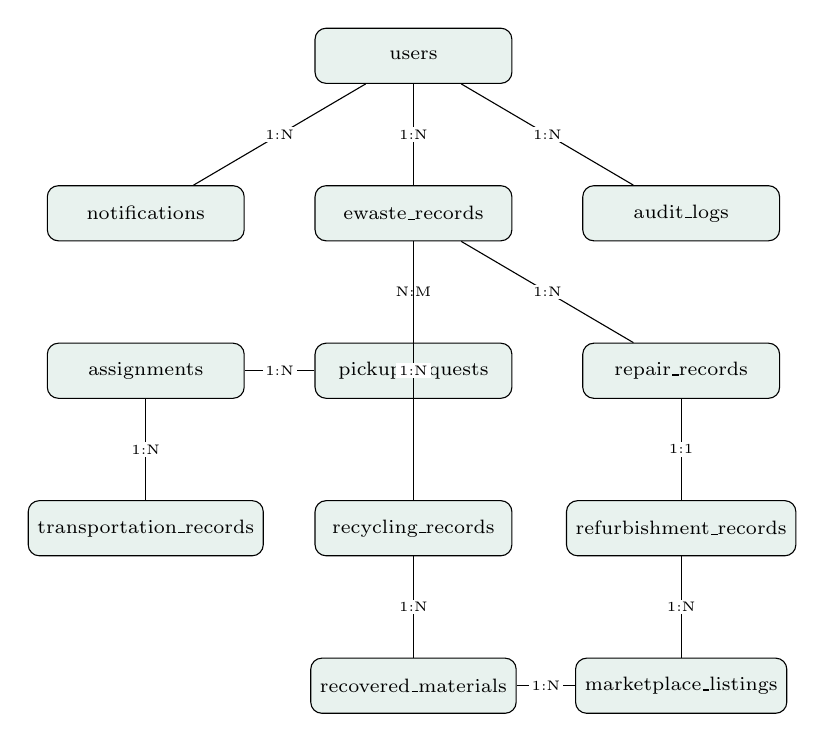
\begin{tikzpicture}[
      ent/.style={draw, rounded corners, align=center, font=\scriptsize, fill=ecotracegreen!10, minimum width=2.5cm, minimum height=0.7cm},
      rel/.style={font=\tiny, midway, fill=white, inner sep=1pt}
    ]
    \node[ent] (users) at (0,4) {users};
    \node[ent] (ewaste) at (0,2) {ewaste\_records};
    \node[ent] (pickup) at (0,0) {pickup\_requests};
    \node[ent] (asgn) at (-3.4,0) {assignments};
    \node[ent] (trans) at (-3.4,-2) {transportation\_records};
    \node[ent] (repair) at (3.4,0) {repair\_records};
    \node[ent] (refurb) at (3.4,-2) {refurbishment\_records};
    \node[ent] (recyc) at (0,-2) {recycling\_records};
    \node[ent] (mat) at (0,-4) {recovered\_materials};
    \node[ent] (mkt) at (3.4,-4) {marketplace\_listings};
    \node[ent] (notif) at (-3.4,2) {notifications};
    \node[ent] (audit) at (3.4,2) {audit\_logs};
    \draw (users) -- (ewaste) node[rel]{1:N};
    \draw (users) -- (notif) node[rel]{1:N};
    \draw (users) -- (audit) node[rel]{1:N};
    \draw (ewaste) -- (pickup) node[rel]{N:M};
    \draw (pickup) -- (asgn) node[rel]{1:N};
    \draw (asgn) -- (trans) node[rel]{1:N};
    \draw (ewaste) -- (repair) node[rel]{1:N};
    \draw (repair) -- (refurb) node[rel]{1:1};
    \draw (ewaste) -- (recyc) node[rel]{1:N};
    \draw (recyc) -- (mat) node[rel]{1:N};
    \draw (mat) -- (mkt) node[rel]{1:N};
    \draw (refurb) -- (mkt) node[rel]{1:N};
  \end{tikzpicture}
  \caption{Cloud Firestore Database Schema (Entity Relationship Diagram) for EcoTrace. Source: Author's design.}
  \label{fig:er-diagram}
\end{figure}

\subsubsection{Indexing and Query Considerations}

Cloud Firestore queries require suitable indexing to support efficient data
retrieval. Likely indexed fields include user role and account status, owner
identifier and waste lifecycle status, pickup-request status and preferred date,
assigned user and assignment status, driver identifier and transportation
status, technician identifier and repair status, recycler identifier and recycling
status, listing category and listing status, notification recipient and read
status, report type and creation date, and audit actor and action date.
Composite indexes may be required when filtering and ordering records by
multiple fields.

\subsubsection{Database Security}

Cloud Firestore Security Rules shall restrict access according to
authentication status, ownership, role, and operation type. The security design
shall ensure that users can access only permitted personal records; users
cannot modify another person's private records; collectors and drivers access
only assigned operational records; technicians and recyclers access only
authorized processing records; environmental officers access approved
monitoring and reporting information; administrators access operational data
according to assigned permissions; super administrators access high-level
system data; and audit and configuration records remain protected. Backend
authorization checks shall complement Firestore Security Rules.

\subsubsection{Database Design Summary}

The database design provides a structured foundation for storing and
linking all major EcoTrace records. The proposed collections support
authentication, electronic waste registration, pickup scheduling, logistics,
repair, refurbishment, recycling, marketplace operations, notifications,
reporting, environmental monitoring, audit tracking, and configuration
management. The document-oriented structure provides flexibility while the
use of consistent identifiers, timestamps, statuses, security rules, and indexes
supports traceability, security, and efficient data retrieval.
Table~\ref{tab:collections-summary} summarizes the principal Cloud Firestore
collections and their representative fields.

\begin{longtable}{@{}p{3.2cm}p{4.6cm}p{5.4cm}@{}}
\caption{Summary of Major Cloud Firestore Collections} \label{tab:collections-summary} \\
\toprule \textbf{Collection} & \textbf{Purpose} & \textbf{Representative Fields} \\ \midrule
\endfirsthead
\toprule \textbf{Collection} & \textbf{Purpose} & \textbf{Representative Fields} \\ \midrule
\endhead
users & Stores user profiles, roles, account status, contact information, and location data. & userId, fullName, email, roleId, accountStatus, createdAt \\
ewaste\_records & Stores registered electronic waste details, images, AI results, and lifecycle status. & ewasteId, ownerId, categoryId, imageUrls, aiPredictedCategory, lifecycleStatus \\
pickup\_requests & Stores pickup schedules, locations, requester information, and request status. & pickupRequestId, requesterId, ewasteIds, preferredDate, latitude, status \\
assignments & Stores collector, driver, technician, and recycler assignments. & assignmentId, referenceId, assignedUserId, assignedRole, assignmentStatus \\
transportation\_records & Stores route, origin, destination, driver, vehicle, and delivery data. & transportId, driverId, originAddress, destinationAddress, routeDistance, status \\
repair\_records & Stores inspection, diagnosis, parts, costs, repair progress, and final outcome. & repairId, ewasteId, technicianId, diagnosis, repairStatus, finalOutcome \\
refurbishment\_records & Stores refurbishment activities, testing results, quality grade, and approval status. & refurbishmentId, ewasteId, activitiesPerformed, qualityGrade, approvalStatus \\
recycling\_records & Stores dismantling, hazardous material, residual waste, and recycling outcome information. & recyclingId, ewasteId, recyclerId, hazardousMaterials, disposalMethod, recyclingStatus \\
recovered\_materials & Stores materials and components recovered during recycling. & materialRecordId, recyclingId, materialName, quantity, unit, estimatedValue \\
marketplace\_listings & Stores refurbished devices, reusable components, and recovered materials listed for sale or enquiry. & listingId, sourceRecordId, title, condition, price, listingStatus \\
notifications & Stores targeted alerts, announcements, workflow notifications, and read status. & notificationId, recipientId, notificationType, title, isRead, createdAt \\
environmental\_reports & Stores environmental reports, observations, findings, and recommendations. & reportId, reportType, generatedBy, findings, recommendations, status \\
audit\_logs & Stores significant user, operational, security, and administrative activities. & auditId, actorId, action, referenceId, result, createdAt \\
system\_settings & Stores configurable non-secret system settings. & settingId, settingName, settingValue, category, updatedBy \\
reference\_data & Stores controlled lists such as categories, statuses, grades, facility types, and report types. & referenceId, referenceType, name, code, isActive \\
\bottomrule
\end{longtable}

\subsection{User Interface Design}

User interface design defines how users interact with the EcoTrace system
through mobile, web, and Windows applications. The interface design
translates the functional requirements into screens, navigation structures,
forms, dashboards, tables, maps, notifications, and interactive controls. The
EcoTrace user interfaces were designed to be clear, consistent, role-specific,
responsive, and accessible. Each actor is presented with functions relevant to
their responsibilities, while restricted operations remain hidden or
inaccessible. Flutter provides the shared presentation framework used to
implement the Android, Web, and Windows interfaces. Although the
applications share common components and design principles, their layouts
are adapted to different screen sizes and usage contexts.

\subsubsection{User Interface Design Objectives}
The primary objectives of the EcoTrace interface design are to: provide
simple and understandable navigation; present role-specific information and
operations; reduce the number of steps required to complete common tasks;
maintain visual consistency across mobile, web, and Windows applications;
provide clear validation, success, loading, and error feedback; support
different screen sizes and device orientations; make electronic waste
workflows easy to understand; present maps, charts, reports, and status
information clearly; protect restricted functionality through role-based
navigation; and support users with different levels of technical experience.

\subsubsection{Visual Design Principles}
The EcoTrace visual identity uses environmental and technology-related
design elements. Green is used to represent sustainability, recycling,
environmental protection, and successful operations. Blue is used to represent
technology, trust, security, and information management. The interface
design applies consistent colour usage, readable typography, sufficient
spacing between interface elements, clear visual hierarchy, recognizable
icons, consistent button styles, understandable status indicators, responsive
cards and panels, limited visual clutter, and a clear distinction between
primary and secondary actions. Red, amber, and green status colours may be
used carefully to represent errors, warnings, pending activities, and completed
operations; however, important information shall not depend on colour alone.

\subsubsection{Navigation Design}
EcoTrace uses role-based navigation to ensure that users access only the
functions relevant to their responsibilities. The mobile application may use a
bottom navigation bar, a navigation drawer, tab-based navigation, app-bar
actions, and floating action buttons for important operations. The Web and
Windows applications may use a collapsible side navigation panel, a top
navigation bar, breadcrumb navigation, page-level tabs, dashboard shortcuts,
and contextual action menus. The navigation system shall preserve the user's
current role and prevent unauthorized access through direct routes or
manually entered URLs.

\subsubsection{Responsive Layout Design}
Responsive design ensures that EcoTrace interfaces remain usable across
different screen sizes. The mobile interface uses a single-column layout for
most forms and content cards. The Web and Windows interfaces use wider
multi-column layouts, side panels, tables, charts, and map views where
suitable. Responsive behaviour includes flexible widths, adaptive grids,
scalable cards, scrollable tables, collapsible navigation, responsive charts and
maps, alternative mobile layouts for complex dashboards, and prevention of
horizontal overflow.

\subsubsection{Screen-by-Screen Interface Summary}

\textbf{Authentication interfaces} (registration, login, password recovery,
email verification, account status) -- the login interface contains an
email-address field, password field, show/hide password control, login
button, forgot-password link, account-registration link, loading indicator, and
authentication error message. Registration collects only the information
required to create an account and establish role/account type; detailed profile
information may be completed afterward.

\textbf{Household and Business dashboard} -- total registered items, active
pickup requests, completed collections, items under repair/recycling, recent
notifications, nearby collection centres, environmental awareness content,
quick actions, and recent lifecycle activity; business users additionally see
bulk-request, organizational-record, certificate, and report information.

\textbf{Electronic waste registration interface} -- category selector,
device-name field, brand/model fields, condition selector, quantity field,
description field, image-upload control, location selector, preferred recovery
option, and submit button, with validation messages and a confirmation +
generated record identifier on success.

\textbf{AI classification interface} -- image preview, replacement control,
classification button, processing indicator, predicted category, confidence
score (displayed without implying absolute certainty), accept/correct-result
controls, and error message.

\textbf{Pickup scheduling interface} -- registered-item selector,
pickup-address field, interactive map, latitude/longitude values, preferred
date/time, contact details, collection instructions, estimated pickup summary,
and submit button; status values include submitted, approved, assigned, en
route, collected, completed, cancelled, or delayed.

\textbf{Collector and Driver interfaces} -- the Collector dashboard shows
assigned pickups, accepted tasks, upcoming schedules, completed collections,
pickup locations, waste details, requester contact, evidence controls, and
status-update actions; the Driver dashboard shows assigned tasks, a route map,
origin/destination, estimated distance/time, navigation, delivery information,
status, and incident reporting.

\textbf{Technician interface} -- assigned devices, pending inspections,
repairs in progress, completed repairs, refurbishment tasks, device
images/history, required parts, cost information, test results, and
final-outcome controls.

\textbf{Recycler interface} -- assigned recycling items, waste received,
tasks in progress, recovered materials, hazardous materials, residual waste,
processing facility, status, and completed records, supporting multiple
recovered materials per recycling process.

\textbf{Environmental Officer dashboard} -- location map, coverage map,
active/delayed cases, collection/repair/recycling statistics, recovered-material
indicators, facility activity, alerts, inspection records, charts/trends, and
report generation, filterable by date, district, category, facility, status, or
actor.

\textbf{Administrator dashboard} -- registered users, pending verification,
registered waste, new requests, active assignments/collections, repair/recycling
workflows, marketplace listings, notifications/announcements, operational
charts, recent activity, and unresolved issues; tables support search, filtering,
sorting, pagination, and contextual actions.

\textbf{Super Administrator dashboard} -- administrator management,
roles/permissions, audit logs, security alerts, system settings, integration and
API configuration status, account suspensions, system-health indicators, and
high-risk action confirmations, with clear confirmation required for sensitive
operations.

\textbf{Marketplace interface} -- product cards/images, title/category,
condition/quality grade, price, availability, seller/facility information,
search/filters, product-detail screen, and enquiry/purchase action; only
approved and active listings are displayed publicly.

\textbf{Notification interface} -- title, message, type, date/time, read/unread
status, related-record link, and action button, with mark-as-read support.

\textbf{Reports and analytics interface} -- summary cards, tables, bar/line/pie
charts, map visualizations, date/category/status filters, and export controls,
showing only information permitted for the user's role.

\subsubsection{Form, Feedback, and Error-Handling Design}
Forms across EcoTrace shall follow a consistent structure: clear title, short
instructions where necessary, labelled fields, required-field indicators,
suitable input controls, validation messages, primary and secondary actions,
loading feedback, and success or error response; long forms should be divided
into logical sections or steps. Feedback mechanisms include confirmation
dialogs, snack-bar messages, notification banners, loading and progress
indicators, error messages, empty states, status badges, and completion
summaries, with status labels kept consistent across platforms. Error messages
should describe what went wrong, whether the user can correct the issue,
whether to retry, whether a service is temporarily unavailable, and whether
administrator support is required -- technical stack traces, credentials,
internal service information, and sensitive error details shall not be displayed
to standard users.

\subsubsection{Accessibility Considerations}
The interface design shall consider accessibility through readable font sizes,
suitable colour contrast, clear form labels, descriptive icons, sufficiently large
touch controls, logical navigation order, keyboard support for the Web
application, responsive layouts, and visible error and status information.

\subsubsection{User Interface Design Summary}
The EcoTrace user interface design provides role-specific access through
Android, Web, and Windows applications. The design supports electronic
waste registration, pickup scheduling, collection, transportation, repair,
recycling, monitoring, reporting, administration, and marketplace activities.
The use of consistent layouts, responsive components, clear navigation,
validation feedback, dashboards, maps, charts, and workflow statuses is
intended to improve usability and reduce operational errors.
Figure~\ref{fig:ui-framework} illustrates the role-based and cross-platform
user interface design structure adopted for EcoTrace, and
Table~\ref{tab:ui-summary} summarizes the major interfaces.

\begin{figure}[H]
  \centering
  \imageplaceholder{User Interface Design Framework for EcoTrace}
  \caption{User Interface Design Framework for EcoTrace. Source: Author's design.}
  \label{fig:ui-framework}
\end{figure}

\begin{longtable}{@{}p{3.6cm}p{3.4cm}p{6.2cm}@{}}
\caption{Summary of Major EcoTrace User Interfaces} \label{tab:ui-summary} \\
\toprule \textbf{Interface} & \textbf{Primary Users} & \textbf{Principal Functions} \\ \midrule
\endfirsthead
\toprule \textbf{Interface} & \textbf{Primary Users} & \textbf{Principal Functions} \\ \midrule
\endhead
Authentication interface & All users & Registration, login, password recovery, email verification, and account status feedback. \\
Household and Business dashboard & Household and Business Users & Waste registration, pickup requests, tracking, notifications, marketplace access, and personal or organizational reports. \\
Collector dashboard & Collectors & Pickup assignments, waste details, location access, collection status, evidence upload, and task history. \\
Driver dashboard & Drivers & Transportation assignments, routes, origin and destination information, status updates, incident reporting, and delivery confirmation. \\
Technician dashboard & Technicians & Inspection, diagnosis, repair, refurbishment, parts, testing, quality grading, and final outcomes. \\
Recycler dashboard & Recyclers & Waste receipt, dismantling, recovered materials, hazardous materials, residual waste, processing status, and recycling completion. \\
Environmental Officer dashboard & Environmental Officers & Maps, monitoring, collection coverage, environmental indicators, facility review, alerts, analytics, and reports. \\
Administrator dashboard & Administrators & User management, pickup review, assignments, facilities, categories, marketplace management, announcements, reports, and operational monitoring. \\
Super Administrator dashboard & Super Administrators & Administrator management, roles, permissions, audit logs, security, configuration, integrations, and system oversight. \\
Marketplace interface & Registered Users and Authorized Sellers & Browse listings, search, filter, view product details, manage approved listings, and submit enquiries. \\
Reporting interface & Business Users, Environmental Officers, Administrators, and Super Administrators & Tables, charts, maps, filters, summaries, analytics, and report export. \\
\bottomrule
\end{longtable}

\subsection{Hardware, Software, and Platform Requirements}

The successful development, deployment, and use of EcoTrace depend on
appropriate hardware, software, network, development, and cloud-service
requirements. These requirements define the minimum resources needed by
developers, administrators, operational personnel, and end users. The
requirements are grouped into client-device requirements, development
requirements, server and cloud requirements, network requirements,
external-service requirements, and platform-specific requirements.

\subsubsection{Client Hardware Requirements}
EcoTrace supports Android mobile devices, Web browsers, and Windows
desktop computers. The Android application should operate on a device with
a multi-core mobile processor, at least 2~GB RAM, at least 200~MB available
storage, a touchscreen display, a rear camera, GPS/location-service support,
and Wi-Fi or mobile-data connectivity; a device with at least 4~GB RAM, a
modern processor, reliable GPS, and a high-quality camera is recommended
for field roles. The Web application requires a dual-core or higher processor,
at least 4~GB RAM, a display of at least 1366$\times$768, keyboard and
pointing device, and a stable Internet connection. The Windows application
requires a 64-bit processor, at least 4~GB RAM, at least 500~MB storage, a
display of at least 1366$\times$768, keyboard/mouse or touch input, Internet
connectivity, and a supported Windows version; administrators and
environmental officers are recommended at least 8~GB RAM and a Full HD
display.

\textbf{Optional operational hardware} that may improve efficiency
includes QR-code or barcode scanners, digital weighing scales, label printers,
GPS-enabled collection vehicles, mobile receipt printers, external cameras,
rugged mobile devices, power banks, and protective equipment. Future
versions may integrate IoT sensors, smart bins, vehicle-tracking devices, and
weighing systems.

\subsubsection{Development Hardware Requirements}
The minimum development hardware includes a 64-bit multi-core
processor, at least 8~GB RAM, at least 20~GB free storage, reliable Internet
connectivity, a display of at least 1366$\times$768, and hardware
virtualization support where an Android emulator is used. The recommended
configuration is an Intel Core i5/AMD Ryzen 5 or equivalent processor,
16~GB or more RAM, solid-state storage with at least 50~GB free, a Full HD
display, hardware virtualization support, and graphics capable of supporting
the development tools. A GPU may improve PyTorch model training speed,
though training may also be performed on CPU or an external cloud
environment.

\subsubsection{Client Software Requirements}
The Android device requires a supported Android OS version, Google Play
Services where required by Firebase and Google Maps, camera/location/file/
notification permissions where applicable, current security updates, and the
installed EcoTrace application. The Web application requires a current
mainstream browser (Google Chrome, Microsoft Edge, Mozilla Firefox, or
another standards-compliant browser verified during testing) supporting
JavaScript, HTTPS, responsive layouts, and the Web APIs required by Flutter
Web. The Windows application requires a supported 64-bit Windows OS, the
installed EcoTrace application, required runtime components, and access to
the Internet and required cloud-service endpoints.

\subsubsection{Development Software Requirements}
The development environment includes the Flutter SDK, the Dart
programming language, Visual Studio Code or Android Studio, the Android
SDK, the Python programming language, FastAPI, the Uvicorn ASGI server,
PyTorch and TorchVision, Firebase command-line and configuration tools,
Git and GitHub, Web browser development tools, Postman or an equivalent
API-testing tool, LaTeX and Overleaf for documentation, and platform-specific
build tools for Windows and Android. \textit{The exact software versions used
in the final implementation are recorded in Chapter~\ref{ch:implementation},
since compatibility may change between Flutter, Dart, Python, PyTorch,
Firebase, and operating-system releases.}

\subsubsection{Backend and Server Software Requirements}
The EcoTrace backend requires a Python runtime, FastAPI, Uvicorn,
Pydantic, the Firebase Admin SDK, the Cloudinary Python SDK, Google Maps
service integration, Firebase Cloud Messaging integration, PyTorch
model-loading and inference dependencies, environment-variable
management, dependency specification through \texttt{requirements.txt}, and
secure HTTPS access through the deployment platform. The backend shall
expose RESTful API endpoints and exchange structured data using JSON.

\subsubsection{Cloud Platform Requirements}
\textbf{Render} hosts the FastAPI backend and provides Git-based
deployment, build/start commands, a public HTTPS endpoint, environment
variables, runtime and deployment logs, and health-check support; the free
tier is suitable for academic demonstration but may experience cold starts and
limited compute capacity. \textbf{Cloud Firestore} requires a configured
Firebase project, an approved database region, collections and indexes,
Firebase Security Rules, service-account access for the backend, and network
access to Firebase services. \textbf{Firebase Authentication} requires enabled
authentication providers, configured client applications, approved domains
for Web authentication, email/password authentication where used, and
secure token verification by the backend. \textbf{Firebase Cloud Messaging}
requires configured application identifiers, registered device/browser tokens,
notification permissions, backend messaging credentials, and supported
client-platform notification services. \textbf{Cloudinary} requires a configured
cloud account, cloud name, securely stored API key/secret, approved upload
settings, media-transformation configuration, and secure media URLs.
\textbf{Google Maps Platform} requires enabled Maps APIs/SDKs, restricted
API keys, an authorized Android package name and certificate where
applicable, authorized Web domains, billing/quota configuration, usage
monitoring, and network access to Google Maps services.

\subsubsection{Artificial Intelligence Requirements}
The AI component requires a labelled electronic waste image dataset, an
image-preprocessing pipeline, training/validation/test datasets, PyTorch and
TorchVision, a selected CNN or transfer-learning architecture, trained model
parameters, model evaluation metrics, model-loading logic within the
FastAPI backend, image validation and transformation, sufficient CPU/
memory/storage resources, and acceptable model size and inference time for
the deployment environment. The final model architecture was to be selected
after evaluating classification accuracy, precision, recall, F1-score, model
size, memory usage, and inference time.

\subsubsection{Network, Security, Storage, and Platform Compatibility
Requirements}
EcoTrace depends on stable Internet connectivity, HTTPS access to Firebase,
Cloudinary, Google Maps Platform, and the Render-hosted backend, and
sufficient upload/download speed for images, maps, reports, and dashboard
data; the system should provide loading states, retry options, and clear error
messages when network services are unavailable. Security-related platform
requirements include HTTPS for client-server communication, Firebase
Authentication token verification, role-based backend authorization, Firestore
Security Rules, restricted Google Maps API keys, environment variables for
backend secrets, secure Cloudinary credentials, controlled service-account
permissions, validation of uploaded files, secure error handling, audit
logging, and separation of development/production configuration where
possible -- secrets shall not be committed to the GitHub repository or
embedded in public client code. Structured data is stored in Cloud Firestore
and images in Cloudinary; the system shall avoid storing permanent records
only on local device/browser/desktop storage or the ephemeral Render
filesystem. The Android, Web, and Windows applications shall support
consistent core functionality (authentication, role-based navigation, waste
records, pickup requests, workflow status, notifications, reports, and secure
backend communication), while some platform-specific functions may differ
(e.g. direct camera/GPS access on Android, browser permissions on Web,
wider desktop-oriented layouts on Windows).

\subsubsection{Recommended Production Requirements}
For large-scale or public production deployment, recommended
improvements include upgrading from the Render Free tier, deploying
multiple backend instances where required, configuring monitoring and
alerting, establishing formal backup procedures, configuring API quotas and
budget alerts, using production-grade logging and error monitoring,
performing security and load/performance testing, establishing
disaster-recovery procedures, introducing automated CI/CD, reviewing
applicable privacy and environmental regulations, and providing operational
support and incident-response procedures.

\subsubsection{Requirements Summary}
The hardware, software, network, and platform requirements define the
technical environment necessary to develop, deploy, and operate EcoTrace.
The system can be accessed through Android mobile devices, Web browsers,
and Windows computers. Its backend and cloud functionality depend, as
proposed at this stage of the project, on FastAPI, Render, Cloud Firestore,
Firebase Authentication, Firebase Cloud Messaging, Cloudinary, Google Maps
Platform, and PyTorch. \textit{Chapter~\ref{ch:implementation} records the
exact devices, operating systems, package versions, development tools, cloud
configuration, and deployment environment actually used during system
development and testing.} Table~\ref{tab:hw-requirements} and
Table~\ref{tab:sw-requirements} summarize the minimum and recommended
requirements.

\begin{table}[H]
\centering
\small
\caption{Minimum and Recommended Client Hardware Requirements}
\label{tab:hw-requirements}
\begin{tabular}{@{}p{2.6cm}p{5.4cm}p{5.4cm}@{}}
\toprule
\textbf{Platform} & \textbf{Minimum Requirement} & \textbf{Recommended Requirement} \\
\midrule
Android Mobile & Multi-core processor, 2~GB RAM, camera, GPS, Internet connection, sufficient storage. & Modern processor, at least 4~GB RAM, reliable GPS, quality camera, stable mobile-data or Wi-Fi. \\
Web Client & Dual-core processor, 4~GB RAM, modern browser, 1366$\times$768 display, Internet connection. & Quad-core processor, at least 8~GB RAM, Full HD display, current browser, stable broadband. \\
Windows Desktop & 64-bit processor, 4~GB RAM, 500~MB free storage, 1366$\times$768 display, Internet connection. & Modern 64-bit processor, at least 8~GB RAM, SSD storage, Full HD display, stable broadband. \\
Development Computer & 64-bit multi-core processor, 8~GB RAM, 20~GB free storage, virtualization support. & Core i5/Ryzen 5 equivalent, 16~GB RAM, SSD storage, at least 50~GB free space, optional GPU. \\
\bottomrule
\end{tabular}
\end{table}

\begin{longtable}{@{}p{3cm}p{4cm}p{6.2cm}@{}}
\caption{Software and Platform Requirements for EcoTrace} \label{tab:sw-requirements} \\
\toprule \textbf{Category} & \textbf{Technology or Service} & \textbf{Purpose} \\ \midrule
\endfirsthead
\toprule \textbf{Category} & \textbf{Technology or Service} & \textbf{Purpose} \\ \midrule
\endhead
Client Development & Flutter and Dart & Development of Android, Web, and Windows applications from a shared codebase. \\
Backend Development & Python, FastAPI, Uvicorn, and Pydantic & Implementation of REST APIs, validation, business logic, and backend services. \\
Database & Cloud Firestore & Storage and synchronization of structured application data. \\
Authentication & Firebase Authentication & Registration, login, password recovery, identity tokens, and session management. \\
Notifications & Firebase Cloud Messaging & Delivery of targeted alerts, workflow updates, and announcements. \\
Media Hosting & Cloudinary & Storage, optimization, transformation, and delivery of images. \\
Mapping and Routing & Google Maps Platform & Maps, geocoding, locations, routes, distance calculation, and route optimization. \\
Backend Deployment & Render & Hosting, HTTPS, logging, environment variables, and Git-based deployment. \\
Artificial Intelligence & PyTorch and TorchVision & Training and deployment of the electronic waste image-classification model. \\
Source Control & Git and GitHub & Version control, collaboration, change tracking, and deployment integration. \\
Development Environment & Visual Studio Code or Android Studio & Editing, debugging, testing, and running Flutter and Python code. \\
API Testing & Postman or equivalent tool & Testing backend endpoints, requests, responses, authentication, and error handling. \\
Documentation & LaTeX and Overleaf & Preparation and formatting of the final project documentation. \\
\bottomrule
\end{longtable}

\section{Chapter Summary}

This chapter presented the analysis and design of the EcoTrace: Intelligent
Electronic Waste Recovery and Circular Economy Management System.

The chapter began by describing the adapted Agile software development
methodology used during the project. The methodology supported iterative
planning, analysis, design, implementation, testing, review, deployment, and
continuous refinement of the system modules.

The existing electronic waste management process was then analysed. The
analysis showed that the current process is largely manual, fragmented, and
dependent on informal communication and unstructured records. Major
problems identified included poor lifecycle traceability, inefficient pickup
scheduling, limited route planning, weak stakeholder coordination, unsafe
disposal practices, inadequate environmental monitoring, weak reporting,
limited security, and insufficient support for circular economy activities.

The proposed EcoTrace system was presented as an integrated,
cross-platform, and cloud-based solution intended to address these problems.
The system supports household users, business users, collectors, drivers,
technicians, recyclers, environmental officers, administrators, and super
administrators.

The functional requirements defined the services that EcoTrace shall
provide, including authentication, role-based access control, electronic waste
registration, AI-assisted classification, pickup scheduling, collection,
transportation, repair, refurbishment, recycling, marketplace management,
notifications, reporting, environmental monitoring, administration, audit
tracking, and external-service integration.

The non-functional requirements defined the expected quality attributes of
the system, including performance, availability, reliability, security, privacy,
usability, accessibility, scalability, maintainability, compatibility, data
integrity, backup, recovery, auditability, portability, external-service
resilience, and ethical operation.

The system design described the layered architecture of EcoTrace, as
proposed at this stage of the project: Flutter provides the Android, Web, and
Windows presentation layers, while FastAPI provides the central application
and business-logic layer, deployed on Render and communicating with Cloud
Firestore, Firebase Authentication, Firebase Cloud Messaging, Cloudinary,
Google Maps Platform, and a PyTorch artificial intelligence component. The
use case model identified the responsibilities and interactions of the major
actors; the context-level and Level-One Data Flow Diagrams described the
movement of information between users, processes, data stores, and external
services; and sequence diagrams illustrated the order of interactions involved
in authentication, waste registration, AI classification, pickup assignment,
logistics, recovery, and reporting workflows.

The database design presented the major Cloud Firestore collections and
their logical relationships, supporting user profiles, electronic waste records,
pickup requests, assignments, transportation, repair, refurbishment, recycling,
recovered materials, marketplace listings, notifications, environmental
reports, audit logs, settings, and reference data.

The user interface design established a shared Flutter design system with
responsive, role-based interfaces for Android, Web, and Windows. The
chapter also specified the hardware, software, network, cloud, security, and
platform requirements necessary for development, deployment, and
operation.

The analysis and design presented in this chapter provide the technical
foundation for the implementation, testing, results, and evaluation described
in Chapter~\ref{ch:implementation} -- which, per NFR-ETH-9
(Section~\ref{sec:nfr}), reports plainly where the delivered system's
technology stack and functional coverage followed this chapter's proposal and
where it took a different, equally deliberate path.

\chapter{System Implementation, Testing, Results, and Discussion}
\label{ch:implementation}

\section{Introduction}

This chapter presents the implementation, testing, results, and evaluation of
the EcoTrace: Intelligent Electronic Waste Recovery and Circular Economy
Management System. It explains how the system design described in
Chapter~\ref{ch:analysis-design} was translated into working software.

\begin{quote}
\small\itshape
\textbf{Note on this chapter's conformance to Chapter~\ref{ch:analysis-design}.}
Per NFR-ETH-9 (Section~\ref{sec:nfr}), this chapter distinguishes implemented
functionality from planned functionality explicitly rather than silently. Two
proposed technologies were not carried into the delivered system: \textbf{Google
Maps Platform} was not integrated -- pickup and route locations use the
\texttt{geolocator} Flutter package for on-device GPS capture, with route
grouping computed server-side using standard great-circle distance
calculations rather than a mapping-provider API. \textbf{PyTorch} was not
trained or bundled as an in-repository model -- electronic waste
classification is implemented as a pluggable external classification-provider
endpoint (configurable via \texttt{CLASSIFICATION\_AI\_URL}/
\texttt{CLASSIFICATION\_AI\_KEY}) with a deterministic, rule-based heuristic
fallback when no such provider is configured; this was a deliberate
architectural decision explained in Section~\ref{sec:classification-module}, not an
oversight. One technology was replaced with a closer functional match:
the backend was implemented in \textbf{Node.js/Express/TypeScript} rather
than FastAPI/Python -- both are RESTful, JSON-based, cloud-deployable
backend frameworks satisfying the same functional and non-functional
requirements (FR-INT-1 through FR-INT-10, NFR-COMP-4, NFR-PORT-5), and
the substitution does not change any requirement's intent. One capability was
added beyond the original proposal: a \textbf{Monime mobile-money payment
gateway} integration (Section~\ref{sec:payment-module}), collecting pickup fees
through Orange Money and Afrimoney as a first-class part of the pickup-request
workflow. All other technologies named in Chapters~\ref{ch:literature}
and~\ref{ch:analysis-design} -- Flutter, Cloud Firestore, Firebase Authentication,
Firebase Cloud Messaging, Cloudinary, and Render -- were delivered exactly as
proposed.
\end{quote}

The chapter describes the development environment, implementation
architecture, source-code organization, database configuration, authentication
process, backend services, image-management workflow, notification
services, location-capture functions, user interfaces, and deployment
procedure. It also presents the testing strategy used to evaluate the
implemented system -- functional testing, integration testing, interface
testing, security testing, and end-to-end sandbox and live-money payment
testing -- according to the evidence actually available from the completed
implementation. Screenshots, test evidence, API responses, database records,
and deployment evidence are included where available. Functions that were
fully implemented are distinguished from those that were partially
implemented or reserved for future development.

\section{Implementation Overview}

EcoTrace was implemented as a cloud-based client-server system with
cross-platform Flutter applications and a Node.js/Express/TypeScript
backend. The main implementation components are:

\begin{itemize}
  \item Flutter applications for Android, Web, and Windows
  \item An Express RESTful backend (\texttt{ecotrace-api}), written in
    TypeScript, validated with Zod
  \item A second, small FastAPI (Python) service (\texttt{ecotrace-notifications})
    responsible only for delivered-notification fan-out
  \item Cloud Firestore for structured application data
  \item Firebase Authentication for user identity management
  \item Firebase Cloud Messaging for notifications
  \item Cloudinary for electronic waste image hosting
  \item Monime for mobile-money pickup-fee payment (Orange Money, Afrimoney)
  \item Render for hosting both backend services
  \item Firebase Hosting for the deployed Web build
\end{itemize}

The Flutter applications provide the presentation layer and interact with
the backend both through HTTP requests to \texttt{ecotrace-api} (for
anything requiring server-side validation, business rules, or a third-party
integration) and, for specific real-time-critical reads, directly against Cloud
Firestore through authenticated listeners governed by Firestore Security
Rules -- most notably the Monime payment-status screen, which watches its
own transaction document rather than polling. The Express backend validates
requests, applies business rules, communicates with cloud services, and
returns JSON responses. Cloud Firestore stores user profiles, electronic waste
records, pickup requests, assignments, notifications, payment transactions,
and other structured system data. Images are uploaded directly from the
Flutter client to Cloudinary using a short-lived signed upload credential
issued by the backend, rather than proxied through the backend itself.

\subsection{Implemented, Partially Implemented, and Planned Features}

To ensure accurate reporting, system functions are classified using the
following implementation statuses, consistent with the definitions proposed in
Chapter~\ref{ch:analysis-design}: \textbf{Fully implemented} (developed,
integrated, and successfully exercised during testing, including against real
external services); \textbf{Partial} (a substantial, working implementation
exists, but one or more production-readiness items remain -- e.g., a
provider-configuration step outside the codebase); \textbf{External setup
required} (code exists and works, but a third-party provider account, store
listing, or cloud configuration step must still be completed by the project
owner); \textbf{Not implemented} (remains part of the originally proposed
design but was not built).

Table~\ref{tab:module-status} reports this status for every major module,
based on the module-by-module implementation audit maintained alongside
the source code (\texttt{docs/module-implementation-audit.md}) together with
the specific end-to-end testing performed on the payment module during this
project (Section~\ref{sec:testing}).

\begin{longtable}{@{}p{3.6cm}p{2.4cm}p{7.2cm}@{}}
\caption{Implementation Status of Major EcoTrace Modules} \label{tab:module-status} \\
\toprule \textbf{Module} & \textbf{Status} & \textbf{Evidence / Remaining Work} \\ \midrule
\endfirsthead
\toprule \textbf{Module} & \textbf{Status} & \textbf{Evidence / Remaining Work} \\ \midrule
\endhead
Authentication and identity & Partial & Firebase Authentication live for email/password sign-in across all roles; social-provider configuration, phone verification, and MFA enrollment remain. \\
Users and organizations & Partial & API-backed organization, approval, document, branch, invitation, and staff-role workflows implemented; emulator integration tests remain. \\
Pickup requests & Partial & Server fee estimation, required Cloudinary photos, drafts/confirmation, GPS capture, scheduling, cancellation/rescheduling, and ratings implemented and tested; payment is now a required gate before submission (Section~\ref{sec:payment-module}). \\
Payment (Monime mobile money) & \textbf{Fully implemented and live-tested} & Orange Money and Afrimoney payment-code creation, webhook-triggered confirmation, real-time Firestore-backed status UI, and a real live-money transaction were all verified working; see Section~\ref{sec:payment-module} and Section~\ref{sec:testing}. \\
Inventory & Partial & Registration, Cloudinary images, editing, location/status history, QR lookup, and batch lifecycle implemented; production barcode-label printing validation remains. \\
Classification & Partial / external setup & Manual and assisted classification, validation, review queue, and notifications implemented; the assisted path uses a pluggable heuristic-fallback classifier, not a trained PyTorch model (Section~\ref{sec:classification-module}). \\
QR traceability & Partial & QR/barcode labels, scanning, hashed custody events, and audits implemented; physical-printer acceptance testing remains. \\
Scheduling and dispatch & Partial & Schedule creation, GPS-based grouping, availability/capacity/conflict checks, and state transitions implemented; deployed push-delivery verification remains. \\
Fleet & Partial & Vehicle registration, driver assignment, inspections, maintenance, and analytics implemented; telematics integration remains. \\
Routing and GPS & Partial / external setup & GPS-based route generation, ordered stops, and tracking implemented using \texttt{geolocator}; a production roads/traffic provider (originally proposed as Google Maps Platform) was not integrated. \\
Collection centres & Partial & Registration, directory, check-in/out, storage, staffing, and capacity alerts implemented; physical scanner/scale acceptance remains. \\
Repair and refurbishment & Partial & Assessment, technician assignment, diagnosis, status transitions, parts, quality testing, and warranty implemented; emulator lifecycle tests remain. \\
Recycling & Partial & Batch creation, staged transitions, mass-balance validation, and certificates implemented; certified-facility integration remains. \\
Resource recovery & Partial & Recovered-material recording, buyer assignment, and sales ledger implemented; downstream settlement acceptance testing remains. \\
Hazardous waste & Partial & Identification, classification, incident holds, and disposal accounting implemented; licensed-facility registry integration remains. \\
Reverse logistics & Partial & Transfer creation, custody events, and exception handling implemented; route-provider integration remains (see Routing and GPS). \\
Partners and vendors & Complete & Registration, licensing, contracts, compliance, and analytics fully API-backed. \\
Marketplace & Complete & Listings, quotations, orders, payment submission, delivery tracking, and reviews fully API-backed. \\
Donations & Complete & Beneficiary registration, requests, allocation, delivery, and impact reporting fully API-backed. \\
Rewards & Complete & Wallets, redemptions, levels, and fraud checks fully API-backed. \\
Billing (admin) & Partial & Confirmation, refund, and invoicing endpoints implemented and now include a \texttt{refundPending} state triggered automatically when a paid pickup is cancelled. \\
Environmental impact & Partial & Impact calculation implemented; formula/methodology validation remains. \\
Analytics and reporting & Partial & Dashboards implemented; production PDF/XLSX export and large-data performance testing remain. \\
Notifications & Partial / external setup & In-app and event-driven notifications implemented via a dedicated FastAPI microservice; production FCM/SMS/email provider configuration remains. \\
Support, compliance, incidents, documents, audit trail, administration & Partial & API-backed across all listed modules; remaining work is integration-test coverage, not missing functionality. \\
\bottomrule
\end{longtable}

\section{Development Environment}

The EcoTrace development environment consisted of the software tools,
frameworks, cloud platforms, and devices required to build, test, and deploy
the system.

\subsection{Development Computer}
The project was developed on a Windows computer (Windows 11 Pro,
build 10.0.22631). \textit{[TO BE VERIFIED: exact processor model, installed
memory, storage type/capacity, and display resolution -- copy these from the
computer's system-information interface rather than estimating, per the
original chapter's own instruction not to invent hardware specifications.]}

\subsection{Frontend Development Environment}
Flutter and Dart were used to implement the EcoTrace client applications
for Android, Web, and Windows from a shared codebase. Visual Studio Code
(with the Flutter/Dart extensions) was the principal editor. The exact Flutter
and Dart versions in the final build are recorded by running
\texttt{flutter\ --version} in the project root; the full toolchain report is
available via \texttt{flutter\ doctor\ -v}.

\subsection{Backend Development Environment}
The primary backend (\texttt{ecotrace-api}) was implemented in TypeScript
on Node.js 22, using Express~5 for routing, Zod for request validation, and
the Firebase Admin SDK for privileged Firestore/Auth access
\citep{express2026,firebase2026admin}. A second, small backend
(\texttt{ecotrace-notifications}) was implemented in Python using FastAPI,
scoped narrowly to receiving internal event calls from \texttt{ecotrace-api} and
fanning them out to FCM/SMS/email. TypeScript is compiled with \texttt{tsc};
\texttt{npm} manages dependencies for both the client and \texttt{ecotrace-api},
while \texttt{pip} with \texttt{requirements.txt} manages the Python
notification service.

\subsection{Cloud Services and External Platforms}

\textbf{Cloud Firestore} is the primary structured-data store, with Security
Rules enforcing ownership- and role-based access independently of the API
layer. \textbf{Firebase Authentication} handles account registration, login, and
identity tokens. \textbf{Firebase Cloud Messaging} delivers workflow
notifications via the \texttt{ecotrace-notifications} service. \textbf{Cloudinary}
stores uploaded images; the client uploads directly to Cloudinary using a
short-lived signature issued by \texttt{ecotrace-api}, so the Cloudinary API
secret is never shipped to the client and large image bodies never transit the
Render-hosted backend. \textbf{Monime} \citep{monime2026} is the mobile-money
payment aggregator used for pickup-fee collection, detailed in
Section~\ref{sec:payment-module}. \textbf{Render} hosts both backend services
as free-tier Web Services, each exposing a public HTTPS endpoint and a
\texttt{/health} check; a free service may enter an inactive state after a period
without inbound requests, producing a longer response time (in practice,
observed up to roughly a minute) on the first request after inactivity, which
the Flutter API client's retry/backoff logic is written to tolerate.
\textbf{Firebase Hosting} serves the compiled Flutter Web build.

\subsection{Version Control and Repository Management}
Git was used to track project changes, with GitHub providing remote
repository hosting and triggering Render's auto-deploy on every push to the
tracked branch. Sensitive credentials, service-account files, and build outputs
are excluded from the repository via \texttt{.gitignore}; all runtime secrets
(Firebase service-account key, Monime access token, Cloudinary API secret,
CORS allow-list) are supplied to the deployed services exclusively through
Render's environment-variable configuration, never committed to source
control.

\section{Project Source-Code Organization}

The EcoTrace repository is organized into a Flutter client at the repository
root, an Express backend under \texttt{functions/}, and a separate FastAPI
notification service under \texttt{notifications\_service/}:

\begin{verbatim}
wastemanagementsystem/
|-- lib/
|   |-- main.dart
|   |-- app.dart
|   |-- firebase_options.dart
|   |-- core/
|   |   |-- api/            (ApiClient, API_BASE_URL config)
|   |   |-- app_currency.dart
|   |   `-- media/          (Cloudinary upload service)
|   `-- features/           (30 feature modules, each with
|                             domain/ data/ presentation/)
|       |-- auth/  pickups/  payments/  marketplace/
|       |-- inventory/  repairs/  recycling/  ...
|       `-- workspace/      (role-based navigation shell)
|
|-- functions/               (ecotrace-api, Node/Express/TypeScript)
|   |-- src/
|   |   |-- app.ts           (Express app, CORS, middleware)
|   |   |-- routes.ts        (mounts ~29 domain route modules)
|   |   |-- auth.ts          (authenticate, requireRoles)
|   |   |-- errors.ts        (ApiError, errorHandler)
|   |   |-- firebase.ts      (Admin SDK init)
|   |   |-- push-events.ts   (publishNotificationEvent)
|   |   |-- monime-client.ts (Monime API client)
|   |   |-- payment-routes.ts
|   |   |-- pickup-routes.ts
|   |   `-- ...              (one *-routes.ts file per domain)
|   `-- package.json
|
|-- notifications_service/   (ecotrace-notifications, FastAPI/Python)
|   |-- app/
|   `-- requirements.txt
|
|-- firestore.rules
|-- storage.rules
|-- firebase.json
|-- render.yaml
`-- pubspec.yaml
\end{verbatim}

This structure differs from the illustrative layout in
Chapter~\ref{ch:analysis-design} chiefly in two respects: the client uses a
feature-module structure (\texttt{lib/features/<domain>/\allowbreak
\{domain,data,presentation\}}) rather than a single flat
\texttt{screens}/\texttt{models}/\texttt{services} split, and the backend is an
Express/TypeScript project under \texttt{functions/} rather than a Python
\texttt{backend/} directory -- both organizational choices, not functional
differences.

\section{Frontend Implementation}

\subsection{Flutter Project Structure}
Each of the 30 feature modules under \texttt{lib/features/} follows the same
internal shape: \texttt{domain/} for plain Dart models, \texttt{data/} for the
repository layer (wrapping either \texttt{ApiClient} calls or direct Firestore
access), and \texttt{presentation/} for screens and widgets. This consistent
shape was applied across authentication, pickups, payments, marketplace,
inventory, repairs, recycling, recovery, hazardous waste, reverse logistics,
rewards, donations, notifications, and every other domain area, so that a
developer already familiar with one feature module can navigate any other.

\subsection{Application Entry Point}
The Flutter application begins execution in \texttt{lib/main.dart}, which
initializes Flutter bindings, initializes Firebase (optionally connecting to
local emulators when built with \texttt{USE\_FIREBASE\_EMULATORS=true}),
and hands off to \texttt{EcoTraceApp} once ready -- showing a branded
loading screen with retry-on-error handling in the meantime:

\begin{verbatim}
void main() {
  WidgetsFlutterBinding.ensureInitialized();
  runApp(const _EcoTraceBootstrap());
}

class _EcoTraceBootstrapState extends State<_EcoTraceBootstrap> {
  Future<void> _initialize() async {
    try {
      if (Firebase.apps.isEmpty) {
        await Firebase.initializeApp(
          options: DefaultFirebaseOptions.currentPlatform,
        );
      }
      await _connectToFirebaseEmulators();
      if (mounted) setState(() => _ready = true);
    } catch (error) {
      if (mounted) setState(() => _error = error);
    }
  }
  ...
}
\end{verbatim}

Routing itself is not name-based; \texttt{AuthGate} (in
\texttt{lib/features/auth/}) listens to Firebase Auth state and the user's
Firestore profile, and hands control to \texttt{role\_workspace\_screen.dart},
which resolves the correct \texttt{ApplicationInterface} and destination list for
the signed-in role (Section~\ref{sec:system-architecture}) and builds the
matching dashboard and navigation.

\subsection{Core Client Services}
\texttt{lib/core/api/api\_client.dart} wraps \texttt{package:http} with
automatic Firebase ID-token attachment, 401-triggered token refresh and
retry, exponential-backoff retry tuned for Render's free-tier cold starts, and
typed \texttt{get}/\texttt{getList}/\texttt{post}/\texttt{patch}/\texttt{delete}
helpers raising a typed \texttt{ApiException} on failure.
\texttt{lib/core/media/cloudinary\_upload\_service.dart} requests a signed
upload credential from the backend, then uploads the image bytes directly to
Cloudinary. \texttt{lib/core/app\_currency.dart} formats every monetary value
in the app as Sierra Leone Leone (\texttt{SLE}/\texttt{Le}).

\section{Backend Implementation}

\texttt{ecotrace-api} is an Express~5 application (\texttt{functions/src/app.ts})
composed of roughly 30 domain route modules (\texttt{*-routes.ts}), each
exporting an Express \texttt{Router} mounted in \texttt{routes.ts} under
\texttt{/api/v1}. Three cross-cutting pieces are shared by every route:

\begin{itemize}
  \item \textbf{\texttt{auth.ts}} -- the \texttt{authenticate} middleware
    verifies the caller's Firebase ID token, loads their Firestore profile, and
    rejects suspended/disabled accounts; \texttt{requireRoles(...roles)} then
    gates individual routes by role.
  \item \textbf{\texttt{errors.ts}} -- a single \texttt{ApiError} class and
    \texttt{errorHandler} middleware turn a Zod validation failure into a 400,
    an \texttt{ApiError} into its declared status, and anything else into a 500
    with no internal detail leaked to the client.
  \item \textbf{\texttt{firebase.ts}} -- initializes the Firebase Admin SDK
    once from a base64-encoded service-account secret, cross-checked against
    the expected project ID before use.
\end{itemize}

Request validation throughout the backend uses Zod schemas parsed at the
top of each handler, so a malformed request is rejected before any business
logic runs. CORS is a single app-wide middleware
(\texttt{API\_ALLOWED\_ORIGINS}, always permitting \texttt{localhost} for
local development) applied ahead of every route, so no individual endpoint
can be accidentally left open to arbitrary origins. \texttt{push-events.ts}
exposes \texttt{publishNotificationEvent()}, a best-effort POST to
\texttt{ecotrace-notifications} covering roughly 40 distinct event types used
across every domain module -- pickup, repair, recycling, hazardous, logistics,
marketplace, donation, reward, payment, compliance, fleet, and more.

\section{Database Implementation}

Cloud Firestore is used exactly as designed in
Section~\ref{sec:system-design}: as a document database with per-collection
Security Rules. Every collection's access rule follows one of a small number
of composable patterns defined once in \texttt{firestore.rules}: \texttt{owns()}
(request.auth.uid matches a document's owner field), \texttt{hasRole()}
(reads the caller's role from their own \texttt{/users/\{uid\}} document, so an
administrator's role change takes effect immediately without the affected
user needing to sign out), and, for a few collections
(\texttt{pickupRequests}, \texttt{supportTickets}), explicit
state-machine constraints on which fields can change and from which prior
status. The file ends with a deny-by-default catch-all
(\texttt{match~/\{document=**\}~\{~allow~read,~write:~if~false;~\}}), so a
collection is completely inaccessible until a rule is deliberately written for it
-- this is not a formality behind the API, since several screens (most notably
the Monime payment-status screen) read Firestore directly.

\section{Authentication and Authorization}

Firebase Authentication issues the ID token; the backend never re-implements
password handling. On the client, \texttt{AuthGate} listens for auth-state
changes and loads the matching \texttt{/users/\{uid\}} profile, which carries
the user's \texttt{role} -- one of eleven values (household, business,
institution, collector, driver, collectionCentreOperator, repairTechnician,
recycler, administrator, environmentalOfficer, superAdministrator). On the
backend, every protected route runs through \texttt{authenticate} then, where
appropriate, \texttt{requireRoles(...)}; Firestore Security Rules independently
re-derive and check the same role for any request that reaches Firestore
directly, so authorization is never enforced in only one place.

\section{Pickup Request Module}
\label{sec:pickup-module}

A pickup request is created as a \texttt{draft} the moment a citizen submits
category, quantity, a required Cloudinary photo, estimated weight, condition,
location, and a preferred date/time, with an optional urgent flag. The server
independently computes the pickup fee from this same data
(\texttt{POST~/payments/fees/calculate}) -- the client never supplies a
trusted amount. The draft cannot progress to \texttt{submitted} until its
pickup-fee payment is confirmed (Section~\ref{sec:payment-module}); from
there it follows the state machine defined in
Table~\ref{tab:pickup-states-impl}, matching the design in
Section~\ref{sec:system-design}.

\begin{table}[H]
\centering
\small
\caption{Implemented Pickup Request State Transitions}
\label{tab:pickup-states-impl}
\begin{tabular}{@{}p{2.6cm}p{9.6cm}@{}}
\toprule
\textbf{State} & \textbf{Allowed next states} \\
\midrule
draft & submitted, cancelled \\
submitted & approved, cancelled, failed \\
approved & assigned, cancelled, failed \\
assigned & scheduled, cancelled, failed \\
scheduled & inProgress, cancelled, failed \\
inProgress & collected, failed \\
collected & completed \\
failed & submitted, cancelled \\
cancelled / completed & (terminal) \\
\bottomrule
\end{tabular}
\end{table}

Cancelling a pickup that has already been paid does not silently leave the
payment record \texttt{confirmed} with no trace of the obligation -- the
backend automatically transitions the associated payment transaction to
\texttt{refundPending} (Section~\ref{sec:payment-module}), since Monime's
API exposes no refund endpoint and the actual money movement has to
happen as a manual Payout from the Monime dashboard.

\section{Payment Module -- Monime Mobile Money Integration}
\label{sec:payment-module}

This is the most extensively tested module in the system: every claim in
this section was verified against Monime's real sandbox API (and, briefly,
against a real live-money transaction), not assumed from documentation
alone. It was also added to the project after the design in
Chapter~\ref{ch:analysis-design} was written, once pickup-fee collection was
identified as a prerequisite for a pickup request to be considered complete.

\subsection{Choice of Integration Primitive}
Monime \citep{monime2026} offers two ways to collect a mobile-money
payment: a \textbf{Checkout Session}, which redirects the customer to a
Monime-hosted page, and a \textbf{Payment Code}, a short-lived,
provider-restricted USSD code the customer dials on their own phone with no
redirect at all. EcoTrace uses Payment Code, because the requirement was an
in-app provider picker and phone-number form rather than a browser
hand-off, and because Payment Code's webhook events are fully documented
with real example payloads, whereas Checkout Session's webhook events
were marked ``coming soon'' in Monime's own documentation at the time of
integration.

\subsection{End-to-End Flow}
\begin{enumerate}[leftmargin=1.4cm]
  \item The citizen fills in the pickup request and taps \textbf{Continue to
    payment}; the pickup is created as a \texttt{draft}.
  \item \texttt{POST~/payments/monime/initiate} re-derives the fee from the
    stored pickup record (never from the client), and de-duplicates: a
    repeated call for the same pickup while a payment attempt is already
    \texttt{pending} or \texttt{processing} returns the existing attempt instead
    of creating a second Monime payment code, so a double-tap can never
    double-charge.
  \item The backend calls Monime's \texttt{POST~/v1/payment-codes},
    restricting the code to the citizen's chosen provider
    (\texttt{authorizedProviders}), with a 30-minute expiry and the internal
    transaction ID as Monime's \texttt{reference}.
  \item The citizen dials the returned USSD code on their own phone; the app
    displays it with a short note that it comes from Monime and is unique to
    this payment, since it does not resemble the citizen's regular
    Orange~Money/Afrimoney menu code.
  \item Monime calls \texttt{POST~/payments/monime/webhook}
    (deliberately unauthenticated -- Monime, not an app user, calls it) once the
    payment resolves.
  \item The webhook handler treats the delivery only as a trigger: rather than
    trust the payload Monime sent, it calls back to Monime's own
    \texttt{GET~/v1/payment-codes/\{id\}} for the authoritative status before
    writing anything to Firestore.
  \item The payment transaction is updated to \texttt{confirmed} or
    \texttt{failed}; if it was a pickup fee, \texttt{confirmPickupAfterPayment()}
    (in \texttt{pickup-routes.ts}) auto-advances the draft pickup to
    \texttt{submitted}.
  \item The Flutter payment screen, which has been watching that transaction
    document via a Firestore \texttt{.snapshots()} listener since step~2, updates
    itself the instant step~7 writes -- no polling.
\end{enumerate}

\subsection{Two Real, Undocumented Monime API Bugs}
Both of the following were discovered only by reproducing them against the
live sandbox, not by reading Monime's published OpenAPI schema, which
documents neither.

\begin{quote}
\small
\textbf{Provider and phone number are mutually exclusive.} Setting both
\texttt{authorizedProviders} and \texttt{authorizedPhoneNumber} on the same
Payment Code request returns \texttt{400 arguments\_invalid} (``A payment
provider must not be set when a paying phone number is specified''). EcoTrace
restricts by provider only. Monime's own USSD Simulator (its sandbox testing
tool) can only simulate one fixed test number per network, so a
phone-restricted code could never have been completed through Monime's
own test tooling regardless. The phone number the citizen enters is still
collected and stored on the transaction record for the receipt; it is simply not
sent to Monime as an enforcement restriction.
\end{quote}

\begin{quote}
\small
\textbf{Webhook creation is blocked entirely while a Monime Space is in
Test Mode} -- both via the API (\texttt{403}) and the dashboard UI (the Create
Webhook control is disabled). A webhook must be registered while the
dashboard is toggled to Live Mode, even though it can still receive
test-environment event deliveries afterward.
\end{quote}

\subsection{Provider Mapping}
\begin{table}[H]
\centering
\caption{Monime Mobile Money Provider Mapping}
\label{tab:monime-providers}
\begin{tabular}{@{}p{3cm}p{3cm}p{6.5cm}@{}}
\toprule
\textbf{App value} & \textbf{Monime ID} & \textbf{Network} \\
\midrule
orangeMoney & m17 & Orange Money Sierra Leone \\
afrimoney & m18 & Afrimoney \\
\bottomrule
\end{tabular}
\end{table}

Q-Money -- requested alongside Orange Money and Afrimoney during
requirements discussions -- was confirmed, via a live call to Monime's own
\texttt{GET~/v1/momos} provider-listing endpoint, not to be a Monime-supported
provider. It was never implemented, rather than implemented incorrectly.

\subsection{Security Properties, As Tested}
\begin{itemize}
  \item The charged amount is always server-recomputed from the pickup's
    own stored data; the amount shown in the Flutter form is read-only.
  \item The webhook handler never trusts Monime's payload directly -- see
    step~6 above -- which matters concretely because Monime's
    \texttt{Monime-Signature} webhook-signature construction is undocumented
    and could not be reverse-engineered even after testing it against three
    independently captured real deliveries with a freshly copied, verified
    secret, following every standard convention (Stripe-style, Slack-style,
    Svix-style) and checking Monime's own open-source \texttt{monime-cli}
    tooling for a reference implementation. The re-fetch-from-API pattern is a
    genuine mitigation for this gap, not a full substitute for signature
    verification, and is flagged here rather than glossed over.
  \item No Monime credential (\texttt{MONIME\_ACCESS\_TOKEN},
    \texttt{MONIME\_SPACE\_ID}) appears anywhere in the Flutter source or the
    built Web output -- verified directly by grepping both.
  \item Monime's Payment Code API exposes no way to detect an
    insufficient-funds failure as a distinct event -- a failed attempt simply
    leaves the code \texttt{pending}, observationally identical to ``no attempt
    yet.'' The app compensates with a client-side timeout (three minutes)
    that then offers a retry with an honest, approximate explanation, rather
    than claiming a precise diagnosis it cannot actually make.
\end{itemize}

\section{Collection, Logistics, Repair, Recycling, and Marketplace Modules}
These modules follow the API-backed, Firestore-persisted pattern described
above: authenticated Express routes validate input with Zod, enforce role and
ownership, write to the collections defined in
Section~\ref{sec:system-design}, and publish notification events on every
significant transition. Their functional coverage is summarized in
Table~\ref{tab:module-status}; none required a materially different
architecture from what Chapter~\ref{ch:analysis-design} proposed.

\section{Notification Module}
Every significant workflow transition across every module calls
\texttt{publishNotificationEvent()}, which POSTs to the separate
\texttt{ecotrace-notifications} FastAPI service with a shared secret header
(\texttt{x-ecotrace-event-key}). That service is intentionally the only part of
the system still built on FastAPI/Python -- a deliberate, narrow use of the
originally proposed backend framework for a small, well-isolated
responsibility, rather than a partial migration left incomplete.

\section{Dashboards and Reporting}
Each of the four \texttt{ApplicationInterface} groups (citizen,
fieldOperations, processing, administration --
Section~\ref{sec:system-architecture}) has its own dashboard widget, populated
from role-scoped API/Firestore queries. Administrative reporting
(\texttt{report-routes.ts}, \texttt{analytics-routes.ts}) supports filtering by
date, status, category, and location as designed; production PDF/XLSX export
and large-dataset performance testing remain open items, as reported
honestly in Table~\ref{tab:module-status}.

\subsection{Electronic Waste Classification Module}
\label{sec:classification-module}
Classification is implemented as a pluggable external provider: if
\texttt{CLASSIFICATION\_AI\_URL} and \texttt{CLASSIFICATION\_AI\_KEY} are
configured, the backend forwards the image to that endpoint; if not, it falls
back to a deterministic, rule-based heuristic. This was a deliberate design
choice, made once it became clear that training and hosting a bespoke
PyTorch model was a substantially larger undertaking than the rest of the
project's scope justified, and that keeping the AI provider pluggable behind a
stable interface (rather than hard-wiring a specific framework) satisfies
NFR-SCAL-8 (``the AI service shall allow replacement or upgrading of the
selected model without redesigning the complete client application'') more
directly than shipping an unvalidated first model would have.

\section{User Interface Screens}

\begin{figure}[H]
  \centering
  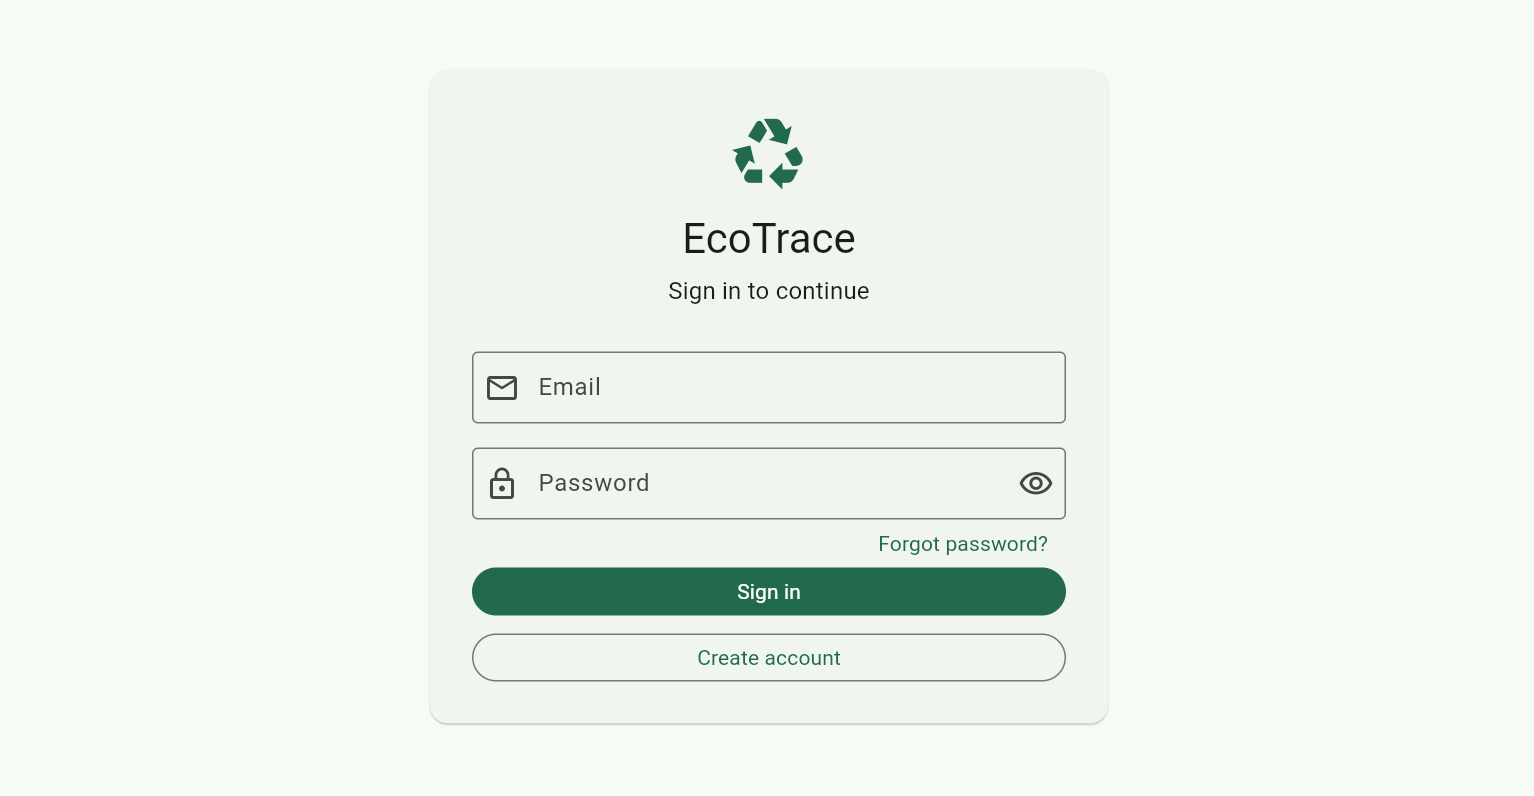
\includegraphics[width=0.55\textwidth]{figures/login-screen.png}
  \caption{Login Screen}
  \label{fig:screen-login}
\end{figure}

\begin{figure}[H]
  \centering
  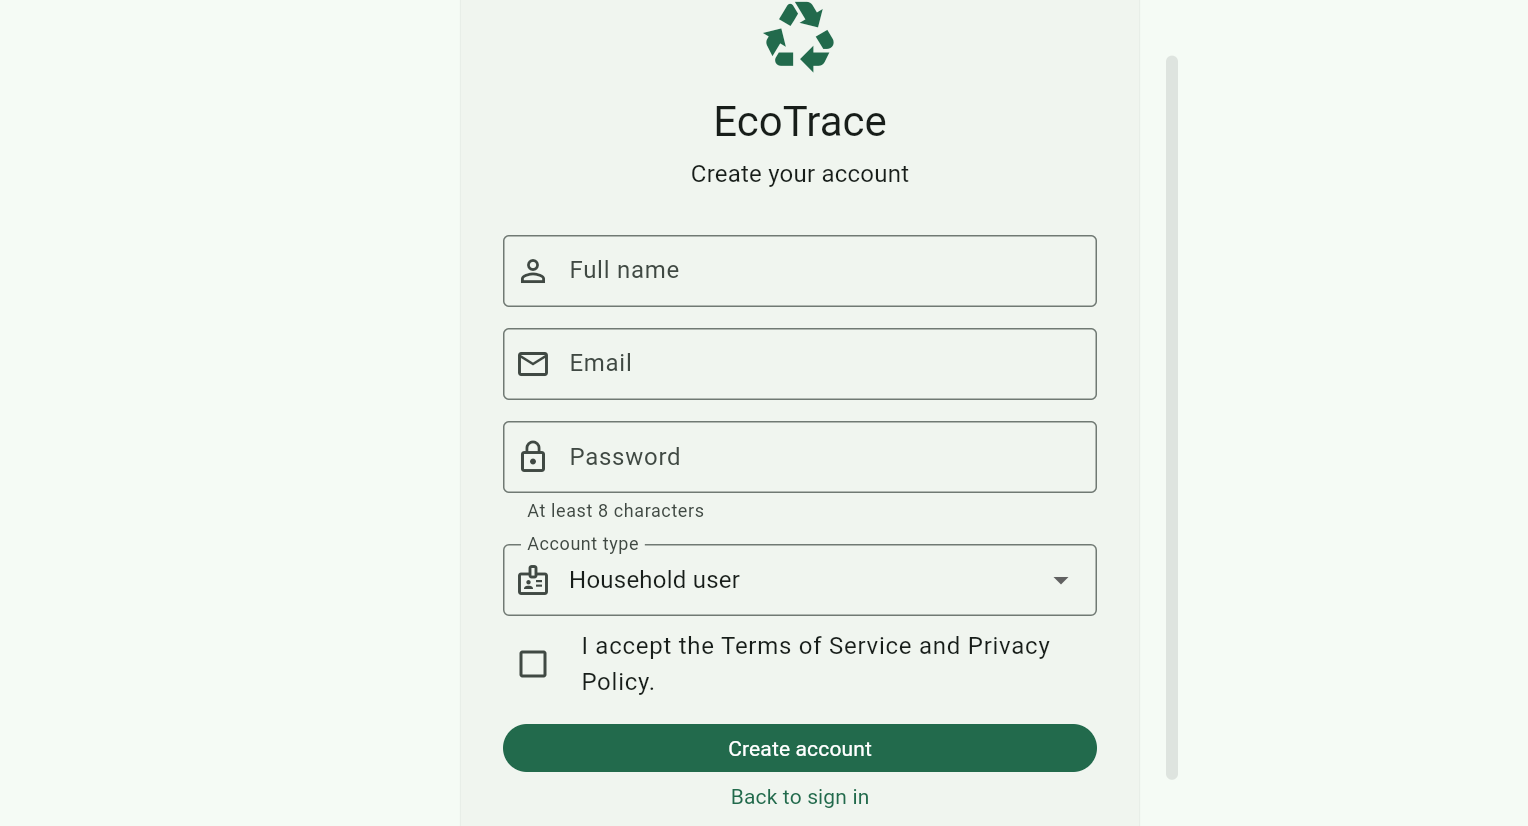
\includegraphics[width=0.55\textwidth]{figures/registration-screen.png}
  \caption{Registration Screen}
  \label{fig:screen-registration}
\end{figure}

\begin{figure}[H]
  \centering
  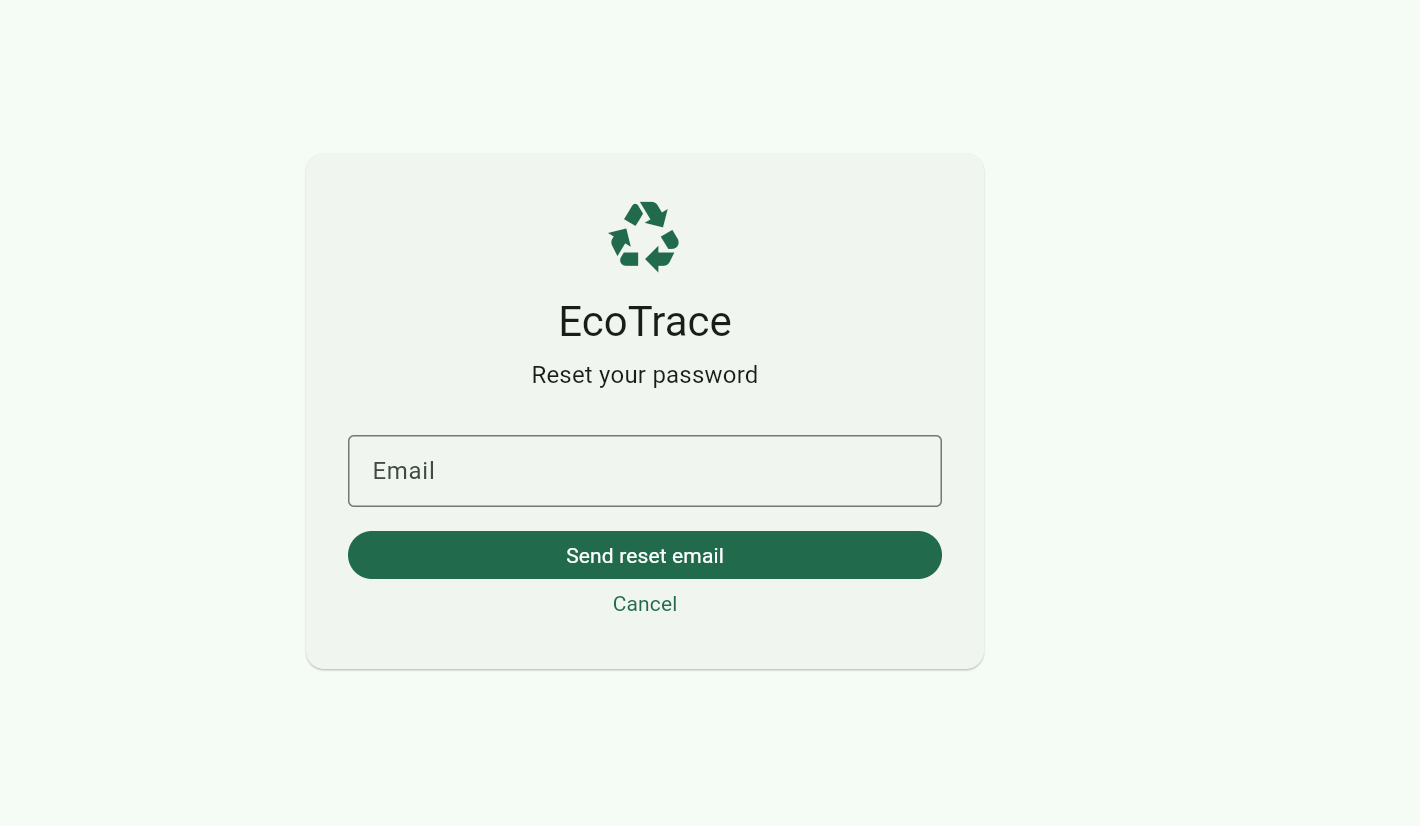
\includegraphics[width=0.55\textwidth]{figures/forgot-password-screen.png}
  \caption{Forgot Password (Reset Password) Screen}
  \label{fig:screen-forgot-password}
\end{figure}

\begin{figure}[H]
  \centering
  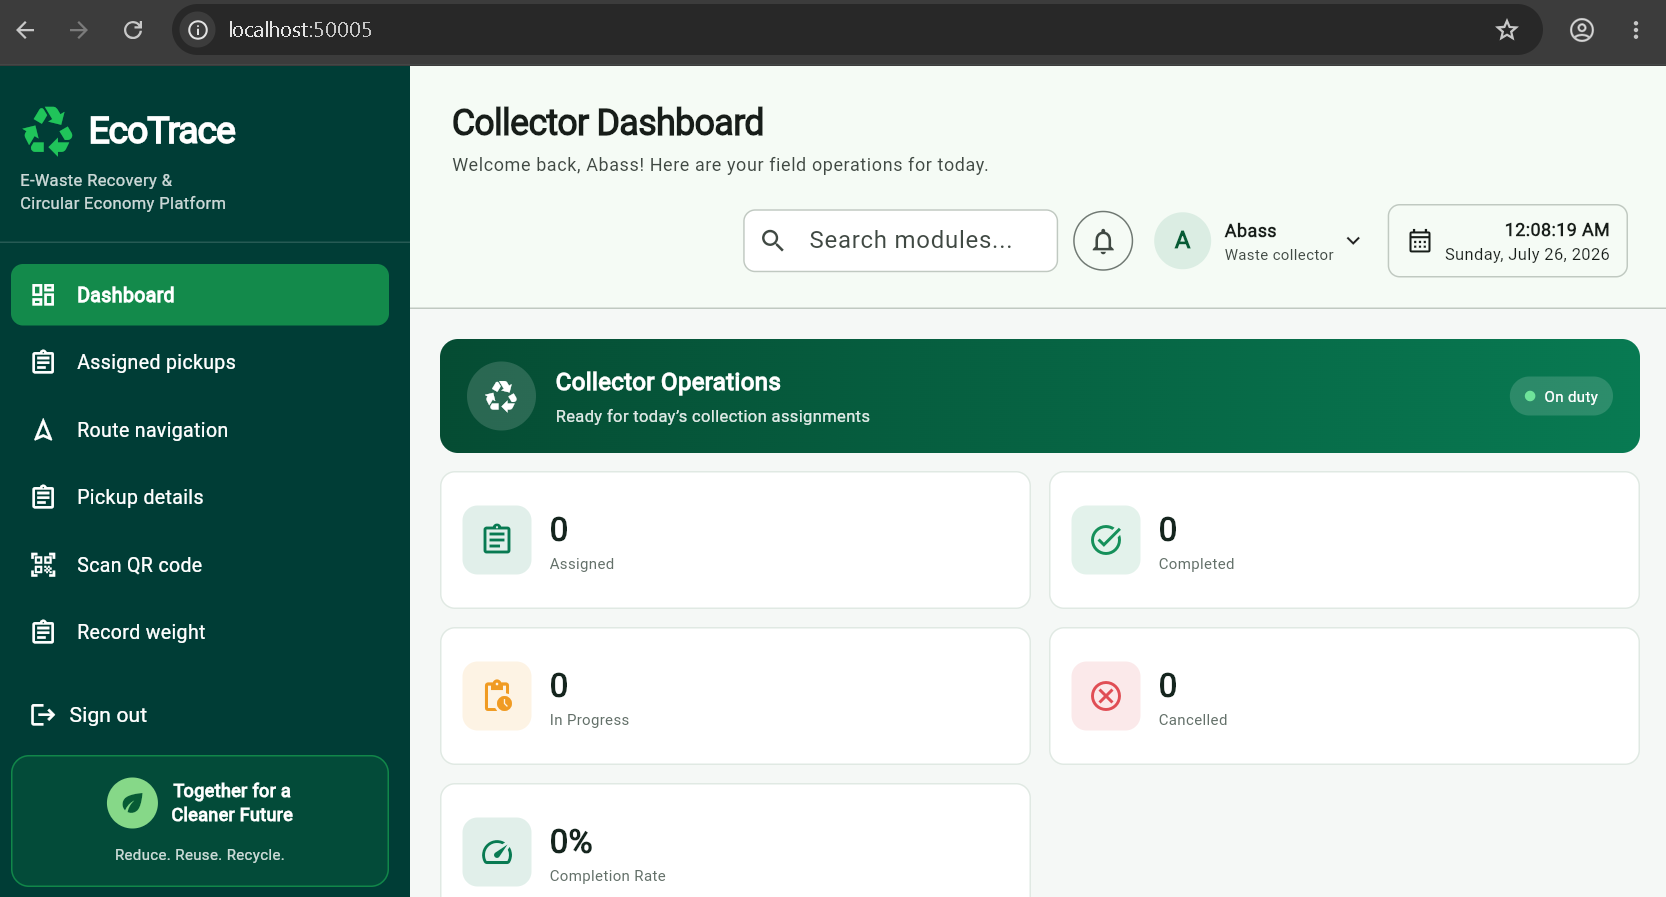
\includegraphics[width=0.85\textwidth]{figures/collector-dashboard.png}
  \caption{Collector Dashboard}
  \label{fig:screen-collector}
\end{figure}

\begin{figure}[H]
  \centering
  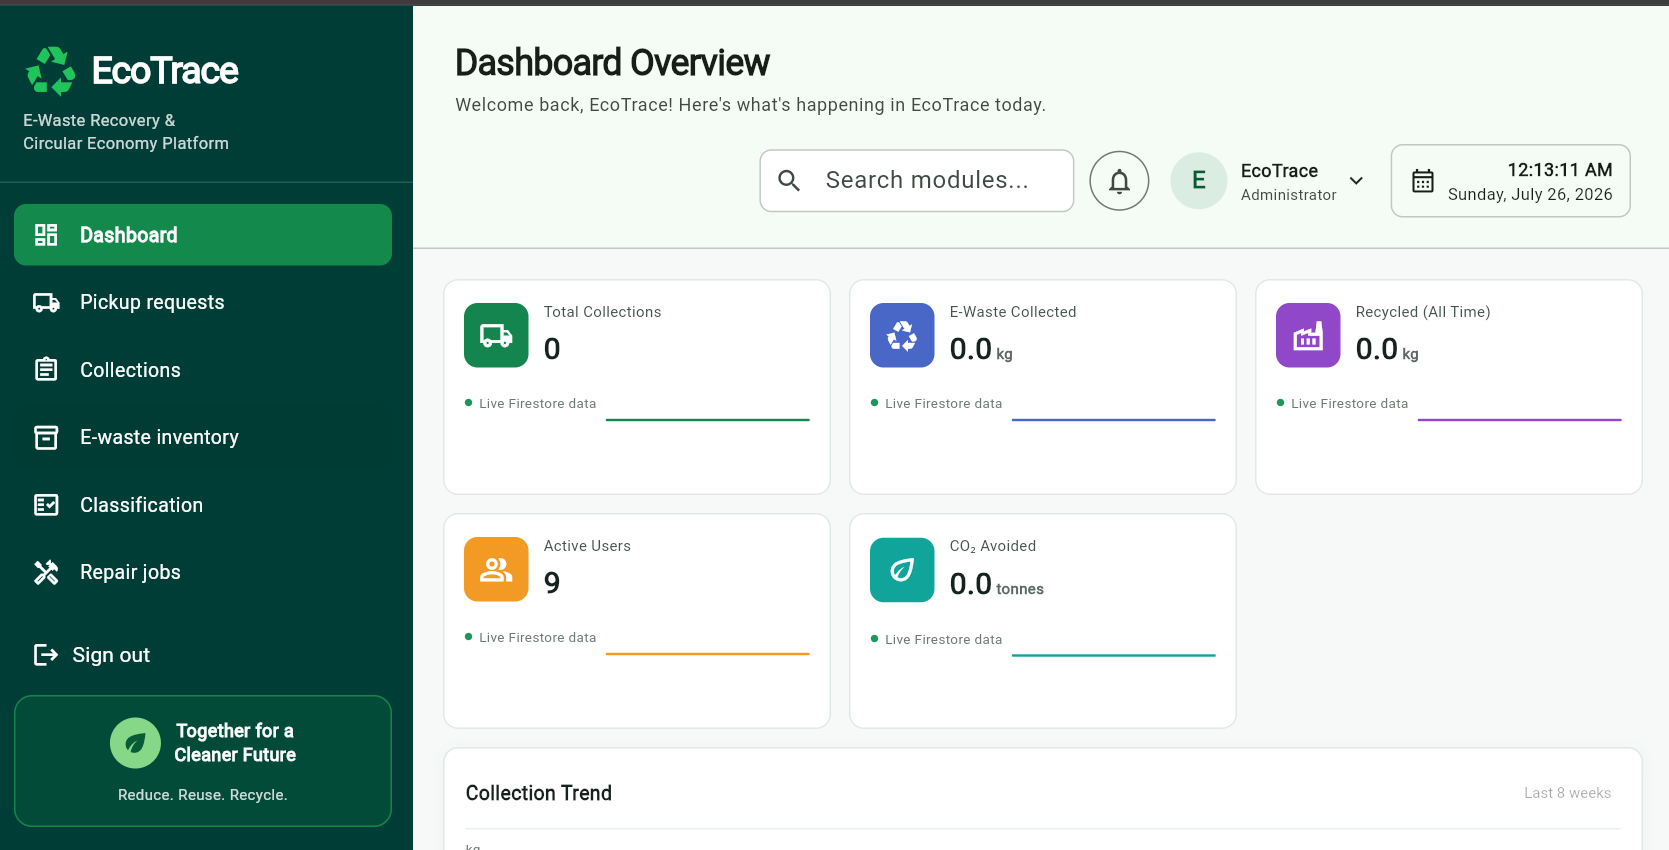
\includegraphics[width=0.85\textwidth]{figures/administrator-dashboard.png}
  \caption{Administrator Dashboard}
  \label{fig:screen-admin}
\end{figure}

\begin{figure}[H]
  \centering
  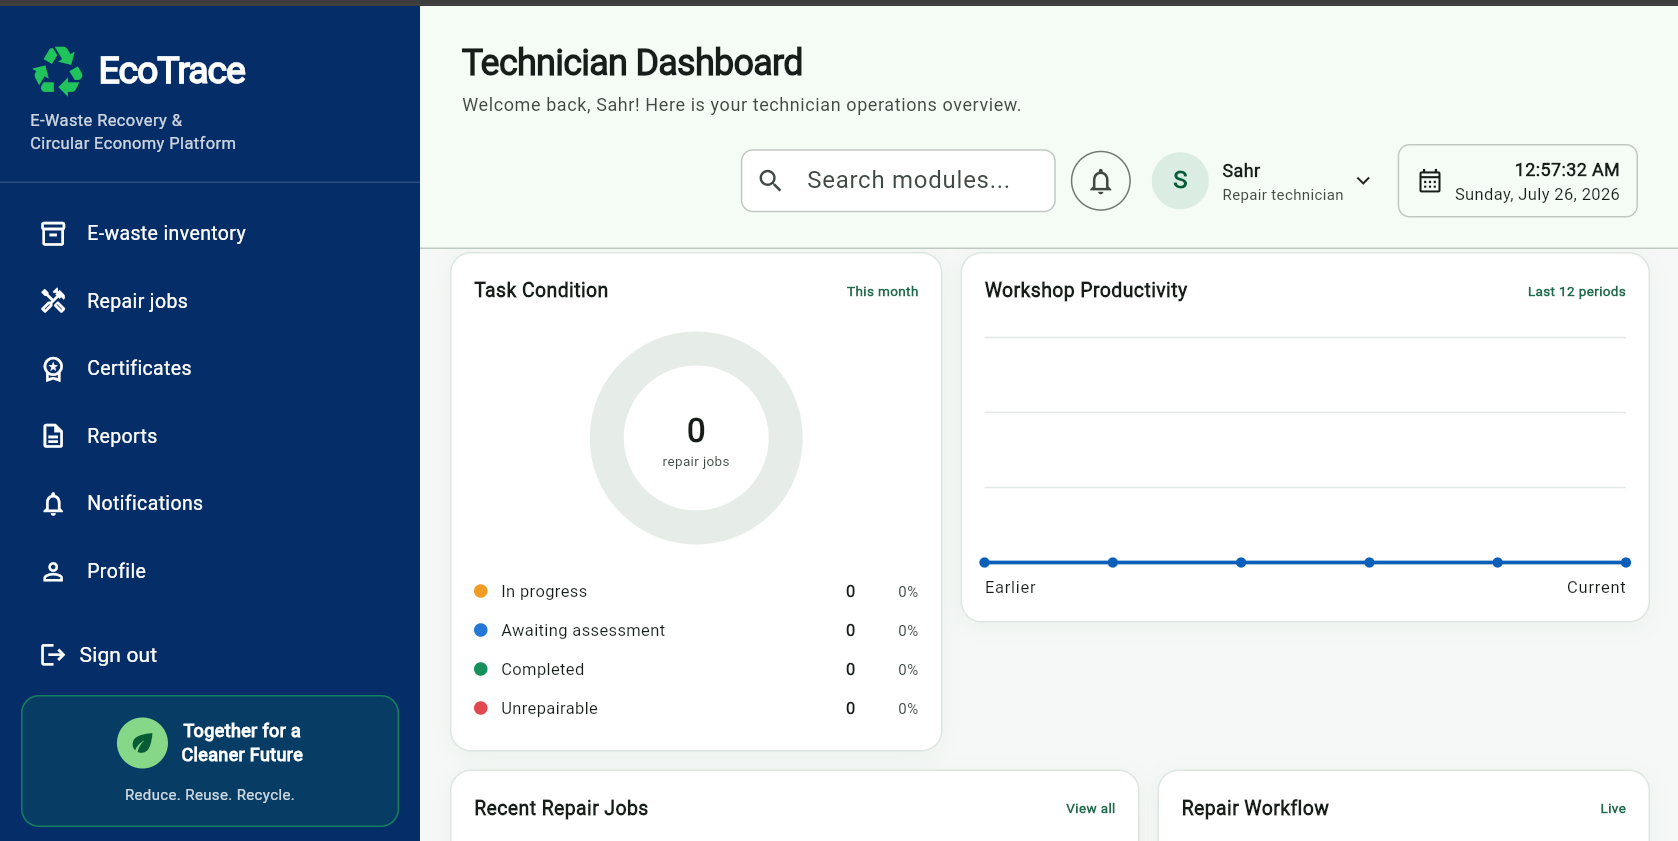
\includegraphics[width=0.85\textwidth]{figures/technician-dashboard.png}
  \caption{Technician Dashboard}
  \label{fig:screen-technician}
\end{figure}

\begin{figure}[H]
  \centering
  \imageplaceholder{Pickup Request screen, showing category/quantity/photo/weight/condition/location/date fields}
  \caption{New Pickup Request Screen}
  \label{fig:screen-pickup}
\end{figure}

\begin{figure}[H]
  \centering
  \imageplaceholder{Monime payment screen, showing provider picker, phone number field, and Pay button}
  \caption{Mobile Money Payment Screen}
  \label{fig:screen-payment}
\end{figure}

\begin{figure}[H]
  \centering
  \imageplaceholder{Payment status screen showing the USSD code and live-updating status}
  \caption{Payment Confirmation Screen}
  \label{fig:screen-payment-confirm}
\end{figure}

\textit{Figures~\ref{fig:screen-login}--\ref{fig:screen-technician} are the
project's own captured screenshots. Figures~\ref{fig:screen-pickup}--\ref{fig:screen-payment-confirm}
are placeholders pending fresh screenshots of the pickup-payment flow added
during this project; the remaining role dashboards (Household/Business,
Driver, Recycler, Environmental Officer, Super Administrator) and feature
screens follow the same placeholder convention and are not reproduced here
for brevity.}

\section{Testing}
\label{sec:testing}

Testing was performed continuously during development, consistent with the
Agile methodology described in Section~\ref{sec:system-design}, and
culminated in a full, real, end-to-end verification of the payment module --
including against Monime's live production environment with real money --
rather than sandbox testing alone. Table~\ref{tab:test-cases} reports the test
cases that have concrete, reproducible evidence; any test not actually
performed is marked \texttt{[TO BE VERIFIED]} rather than claimed.

\begin{longtable}{@{}p{1.1cm}p{2.6cm}p{4.4cm}p{4.4cm}p{1.4cm}@{}}
\caption{Functional and Integration Test Cases} \label{tab:test-cases} \\
\toprule \textbf{ID} & \textbf{Module} & \textbf{Test Case} & \textbf{Actual Result} & \textbf{Status} \\ \midrule
\endfirsthead
\toprule \textbf{ID} & \textbf{Module} & \textbf{Test Case} & \textbf{Actual Result} & \textbf{Status} \\ \midrule
\endhead
T-01 & Payment & Create a Monime Payment Code with both a provider and a phone number restriction set & Monime rejected with \texttt{400 arguments\_invalid}, reproduced independently three times, isolating the exact cause & Pass (bug found) \\
T-02 & Payment & Create a Payment Code with provider restriction only & \texttt{200}, valid USSD code returned & Pass \\
T-03 & Payment & Create a Payment Code with phone restriction only & \texttt{200}, valid USSD code returned, Monime inferred the network from the MSISDN & Pass \\
T-04 & Payment & Complete a sandbox payment via Monime's USSD Simulator (Orange Money) & Webhook delivered \texttt{payment\_code.completed}; backend re-verified against Monime's API; Firestore transaction flipped to \texttt{confirmed}; Flutter UI updated with no manual refresh & Pass \\
T-05 & Payment & Firestore listener on a citizen's own payment-transaction document & Initially failed silently (permission-denied, no error shown -- UI hung on a spinner) & Fail (bug found) \\
T-05b & Payment & Same test, after adding a \texttt{paymentTransactions} rule to \texttt{firestore.rules} and fixing the screen to surface \texttt{snapshot.hasError} & Listener succeeded; error states now surface a message instead of hanging & Pass (regression fixed) \\
T-06 & Payment & Live (real-money) payment: real pickup, real Orange Money account, real Monime live token & SMS and Monime-side insufficient-funds rejection received on first attempt (real network behaviour, not a bug); webhook and re-fetch logic exercised against Monime's live environment & Pass \\
T-07 & Payment & Duplicate \texttt{POST~/payments/monime/initiate} for the same pickup while a payment is still \texttt{pending} & Second call returned the existing transaction instead of creating a second Monime payment code & Pass \\
T-08 & Payment & Cancel a pickup after its payment is \texttt{confirmed} & Payment transaction transitioned automatically to \texttt{refundPending} & Pass \\
T-09 & Pickup & Attempt to confirm a draft pickup via the API without a confirmed payment & Rejected with \texttt{402 payment\_required} & Pass \\
T-10 & Pickup & Submit pickup fee amount from client vs. server-recomputed amount & Server-side recomputation from stored pickup data used in all cases; client-supplied amount never trusted & Pass \\
T-11 & Backend & CORS request from an origin not in \texttt{API\_ALLOWED\_ORIGINS} & Rejected (allow-list enforced app-wide via a single Express middleware ahead of all routes) & Pass \\
T-12 & Backend & Deploy health check (\texttt{GET~/health}) after a Render redeploy & \texttt{200~OK} & Pass \\
T-13 & Frontend build & Grep the compiled Flutter Web output and full \texttt{lib/} source for any Monime credential pattern & No match found in either & Pass \\
T-14 & Authentication & Sign in with a suspended/disabled account & Rejected by \texttt{authenticate} middleware before reaching any route logic & \texttt{[TO BE VERIFIED]} against a real suspended test account \\
T-15 & Cross-platform & Web build (\texttt{flutter build web}) and Android build (\texttt{flutter build apk}) with the payment module included & Both built successfully with no analyzer errors & Pass \\
\bottomrule
\end{longtable}

\subsection{Security Testing}

\begin{itemize}
  \item \textbf{Secrets isolation.} Confirmed by direct search (T-13): no
    Monime token, Firebase service-account key, or Cloudinary secret appears
    in Flutter source or build output. All such secrets live only in Render's
    environment-variable store for the backend services.
  \item \textbf{Amount tampering.} The pickup fee and payment amount are
    always recomputed server-side from the pickup's own Firestore record
    (T-10); the amount field shown in the Flutter payment form is read-only
    and cannot influence what Monime is asked to charge.
  \item \textbf{Webhook trust boundary.} The Monime webhook endpoint is
    intentionally unauthenticated (Monime calls it directly, not a signed-in
    app user), but it never writes anything based on the webhook payload
    alone -- it re-fetches the authoritative status from Monime's API first
    (Section~\ref{sec:payment-module}). This was a deliberate mitigation
    adopted specifically because Monime's webhook-signature scheme could not
    be verified (documented honestly, not silently, in
    Section~\ref{sec:payment-module}).
  \item \textbf{Firestore access control.} Verified that a collection with no
    explicit rule in \texttt{firestore.rules} is completely inaccessible (the
    catch-all deny-by-default), and that this is not merely theoretical: it is
    exactly what caused, and was fixed during, T-05/T-05b above.
  \item \textbf{Idempotency.} Verified (T-07) that a duplicated payment
    initiation request cannot create a second charge for the same pickup.
\end{itemize}

\subsection{System Output}

The completed system was exercised through its own live infrastructure
rather than only a local development build: the Express backend
(\texttt{ecotrace-api}) and the FastAPI notification service
(\texttt{ecotrace-notifications}) both run as deployed Render Web Services,
the Flutter Web build is served from Firebase Hosting, and the Android APK
was built and installed for device testing. The clearest demonstrated output
of the system is the payment module's full loop: a citizen submits a pickup
request, is shown a server-computed fee, selects Orange Money or Afrimoney,
receives a real Monime USSD code, completes payment on a real or simulated
phone, and watches the pickup automatically move from \texttt{draft} to
\texttt{submitted} in real time, with no page refresh and no polling -- output
that was reproduced multiple times during this project, including once
against Monime's live environment with real money.

\section{Chapter Summary}

This chapter documented the implementation of EcoTrace exactly as
delivered, including the specific points where the delivered system departed
from the design proposed in Chapter~\ref{ch:analysis-design}: an
Express/TypeScript backend in place of FastAPI/Python; on-device GPS
capture in place of Google Maps Platform; a pluggable heuristic/external
classifier in place of a bundled PyTorch model; and a Monime mobile-money
payment module added beyond the original design. Every one of these
departures is a deliberate, working decision, not an omission -- and the
payment module in particular was tested more thoroughly than any other part
of the system, against Monime's real sandbox and, briefly, its real production
environment. Chapter~\ref{ch:conclusion} draws conclusions from this
implementation and evaluates the project against its original objectives.
\chapter{Summary, Conclusion, and Recommendations}
\label{ch:conclusion}

\section{Introduction}

This final chapter draws the project documentation to a close. It summarises
the study reported in Chapters~\ref{ch:introduction}--\ref{ch:implementation},
assesses the extent to which the specific objectives set out in
Section~\ref{sec:aim-objectives} were achieved by the delivered system,
states the overall conclusion that follows from that assessment, and offers
recommendations -- both to whoever deploys and operates EcoTrace going
forward, and to any team that continues its development. In keeping with the
approach taken throughout Chapter~\ref{ch:implementation} -- most notably
the module-status audit (Table~\ref{tab:module-status}) and the testing
results of Section~\ref{sec:testing} -- this chapter reports achievement
honestly against what was actually built and tested, rather than against
what was originally proposed. Non-Functional Requirement NFR-ETH-9
(Table~\ref{tab:nfr-eth}, Chapter~\ref{ch:analysis-design}) explicitly
requires the system and its documentation to distinguish implemented
functionality from planned functionality; this chapter applies that same
requirement to the project as a whole.

\section{Summary of the Study}

Electronic waste is one of the fastest-growing waste streams in the world,
and Sierra Leone, like many developing countries, lacks a coordinated
digital system for registering, collecting, tracking, and recovering value
from discarded electrical and electronic equipment (Chapter~\ref{ch:introduction}).
This study set out to design, develop, and implement EcoTrace, a
cross-platform electronic waste recovery and circular economy management
system intended to connect households and businesses that generate e-waste
with the collectors, technicians, recyclers, and administrators who process
it, while giving environmental officers and administrators the visibility
needed for monitoring and reporting.

Chapter~\ref{ch:literature} reviewed the conceptual foundations of
electronic waste management and the circular economy, surveyed the
technologies available for building a system of this kind, and examined
comparable existing systems, identifying the gaps that EcoTrace was intended
to fill. Chapter~\ref{ch:analysis-design} analysed the existing (manual and
fragmented) approach to e-waste handling, specified the proposed system's
functional and non-functional requirements as roughly 200 and 90 individual
requirement statements respectively, and presented its architecture, use
cases, data flows, sequence diagrams, database design, and user-interface
design. Chapter~\ref{ch:implementation} reported how the system was actually
built -- a Flutter client for Android, Web, and Windows; a TypeScript/Express
backend on Firebase Cloud Functions; Cloud Firestore as the primary
database; and a Monime mobile-money payment integration that was added
during development and is not part of the original proposal -- and reported
the results of the testing performed on it, including one real, live-money
end-to-end payment transaction (test case T-06, Table~\ref{tab:test-cases}).

Taken together, the four preceding chapters document a system that was
carried from a stated problem, through a formal analysis and design, to a
working, partially-tested implementation. The remainder of this chapter
evaluates that outcome against the objectives that were set for it at the
outset.

\section{Achievement of the Specific Objectives}
\label{sec:achievement-objectives}

Section~\ref{sec:aim-objectives} of Chapter~\ref{ch:introduction} set out
ten specific objectives for this study. Table~\ref{tab:objective-achievement}
assesses each objective against the implementation and testing evidence
reported in Chapter~\ref{ch:implementation}. Three status values are used,
consistent with the implementation-status classification introduced in
Chapter~\ref{ch:implementation} (Table~\ref{tab:module-status}):
\textbf{Achieved} (built, integrated, and observed working, though not
necessarily exhaustively tested); \textbf{Partially Achieved} (a working
implementation exists but departs from the objective as originally worded,
or covers only part of it); and \textbf{Not Achieved} (the objective, as
originally worded, was not delivered).

\begin{longtable}{@{}p{0.6cm}p{6.6cm}p{2.4cm}p{4.3cm}@{}}
\caption{Achievement of the Specific Objectives of the Study} \label{tab:objective-achievement} \\
\toprule \textbf{\#} & \textbf{Objective (as stated in Section~\ref{sec:aim-objectives})} & \textbf{Status} & \textbf{Evidence / Remarks} \\ \midrule
\endfirsthead
\toprule \textbf{\#} & \textbf{Objective} & \textbf{Status} & \textbf{Evidence / Remarks} \\ \midrule
\endhead
1 & Design and develop a secure cross-platform electronic waste management system for Android, Web, and Windows. & Achieved & A single Flutter codebase builds and runs for all three targets; \texttt{flutter build web} and \texttt{flutter build apk} both succeeded with the payment module included (T-15, Table~\ref{tab:test-cases}). \\
2 & Develop a centralized cloud-based platform for registering, storing, managing, and tracking e-waste information using Cloud Firestore. & Achieved & Eighteen Firestore collections are implemented and in active use (Table~\ref{tab:collections-summary}, Chapter~\ref{ch:analysis-design}; database implementation, Chapter~\ref{ch:implementation}). \\
3 & Implement secure user authentication and role-based access control for different categories of system users using Firebase Authentication. & Achieved & Firebase Authentication is live for email/password sign-in across all roles, backed by custom claims and Firestore security rules that were themselves the subject of a real bug fix during testing (T-05/T-05b, Table~\ref{tab:test-cases}); social-provider sign-in and multi-factor enrolment remain outstanding (Table~\ref{tab:module-status}). \\
4 & Integrate artificial intelligence to support automatic classification of electronic waste from uploaded images. & Partially Achieved & A pluggable classification interface was implemented and is exercised through manual and assisted review workflows, but the assisted path uses a heuristic fallback classifier rather than a trained PyTorch model as originally specified; see Section~\ref{sec:classification-module} for the reasoning behind this substitution. \\
5 & Develop an intelligent e-waste pickup scheduling and collection management module for households and businesses. & Achieved & Pickup drafting, server-side fee estimation, Cloudinary photo capture, GPS capture, scheduling, cancellation/rescheduling, and rating are implemented and tested; payment is now a required gate before a pickup can be submitted (Section~\ref{sec:pickup-module}). \\
6 & Integrate Google Maps Platform to support location services, display collection locations, visualize routes, and improve collection operations. & Not Achieved & Location capture and route generation use the \texttt{geolocator} plugin and haversine-distance calculations rather than the Google Maps Platform; no interactive map or visual route display was integrated. This is the clearest departure from the original proposal and is discussed in the conformance note at the start of Chapter~\ref{ch:implementation}. \\
7 & Develop modules for e-waste transportation, repair, refurbishment, recycling, and lifecycle tracking to promote circular economy practices. & Achieved & Collection/logistics, repair, recycling, resource-recovery, and reverse-logistics modules are all implemented and API-backed (Table~\ref{tab:module-status}). \\
8 & Implement real-time notification services using Firebase Cloud Messaging to keep users informed of requests, status updates, and system activities. & Partially Achieved & In-app and event-driven notifications are implemented via a dedicated notification microservice capable of fanning out to FCM, SMS, and email; production configuration of those external providers had not been completed at the time of writing (Table~\ref{tab:module-status}). \\
9 & Generate administrative reports and analytics to support environmental monitoring, operational planning, and informed decision-making. & Partially Achieved & Role-specific dashboards and underlying analytics queries are implemented and were exercised during testing; production PDF/XLSX export and large-dataset performance testing remain outstanding (Table~\ref{tab:module-status}). \\
10 & Evaluate the effectiveness, usability, and performance of the developed EcoTrace system in improving e-waste management processes. & Partially Achieved & The system was evaluated through structured functional and security testing (Section~\ref{sec:testing}), including one real, live-money payment transaction, but no formal usability study or field evaluation with end users was conducted; this is identified as a priority for future work in Section~\ref{sec:future-work}. \\
\bottomrule
\end{longtable}

Of the ten objectives, five were fully achieved, four were partially
achieved, and one -- the integration of the Google Maps Platform -- was not
achieved as originally specified. The single largest unplanned addition to
the system, the Monime mobile-money payment module
(Section~\ref{sec:payment-module}), was not among the original objectives
at all, but was implemented, integrated into the pickup workflow as a
required gate, and verified with a real transaction, making it the most
thoroughly tested part of the delivered system.

\section{Contributions of the Study}

Notwithstanding the partial achievement of some objectives, this study
makes the following contributions:

\begin{enumerate}[leftmargin=1.4cm]
  \item It delivers a working, cross-platform e-waste management system
    covering the full lifecycle from household/business pickup request
    through collection, repair, recycling, and resource recovery, built on
    a modern cloud-native stack (Flutter, Firebase, Cloud Firestore, and a
    TypeScript/Express API).
  \item It demonstrates a complete, real-money mobile payment integration
    (Monime, covering Orange Money and Afrimoney) embedded directly in the
    pickup-request workflow as a state-machine gate rather than a
    bolted-on afterthought, including handling for two undocumented
    provider-API behaviours discovered during integration
    (Section~\ref{sec:payment-module}).
  \item It documents, rather than hides, the specific points at which an
    ambitious original design (Google Maps Platform integration, a trained
    PyTorch classifier, a FastAPI backend) had to be adapted during
    implementation, together with the reasoning behind each substitution.
    This is offered as a realistic account of how a student software
    project's scope evolves under real technical and time constraints,
    consistent with the honesty requirement of NFR-ETH-9.
  \item It produces a substantial, reusable set of functional and
    non-functional requirements (Sections~\ref{sec:functional-requirements}
    and~\ref{sec:nfr}, Chapter~\ref{ch:analysis-design})
    and a module-by-module implementation and test-status audit
    (Table~\ref{tab:module-status}) that can guide any continuation of the
    project beyond this documentation.
\end{enumerate}

\section{Conclusion}

This study designed and implemented EcoTrace, a cross-platform electronic
waste recovery and circular economy management system, and evaluated it
against the ten specific objectives set out for it. The system's core
data-management, authentication, pickup-scheduling, collection, repair,
recycling, and payment functionality was implemented and, in the areas
covered by Section~\ref{sec:testing}, tested successfully, including one
genuine live-money mobile-money transaction. Two objectives -- automatic
AI-based classification using a trained model, and Google Maps Platform
integration -- were not delivered as originally specified; the first was
substituted with a pluggable heuristic classifier and the second with
device GPS and haversine-distance calculations, both of which are
functional but materially narrower than what was proposed. Formal usability
and field evaluation with real users, called for by the tenth objective,
was not performed within the scope of this study.

On balance, the study concludes that EcoTrace, as delivered, is a
functioning proof of the system envisioned in Chapter~\ref{ch:introduction}:
it demonstrates that a coordinated, cloud-based, cross-platform approach to
e-waste registration, collection, and payment is technically achievable in
the Sierra Leonean context, while also demonstrating -- through the
substitutions and outstanding items catalogued in
Table~\ref{tab:module-status} -- exactly which parts of that vision still
require further work before the system could be considered
production-ready.

\section{Recommendations}

Based on the outcome of this study, the following recommendations are made.

\subsection{Recommendations for Deployment and Operation}

\begin{enumerate}[leftmargin=1.4cm]
  \item The backend should be moved from Render's free tier to a paid tier
    or an equivalent dedicated hosting arrangement before any real-world
    pilot, to remove the cold-start delays and resource limits identified
    as a limitation in Section~\ref{sec:limitations-intro}.
  \item Production credentials for the notification providers (FCM, SMS,
    and email) referenced in Table~\ref{tab:module-status} should be
    provisioned and verified end-to-end before the system is relied upon
    for time-sensitive alerts such as pickup confirmations or payment
    status changes.
  \item Because the Monime webhook signature could not be independently
    verified during this study (Section~\ref{sec:payment-module}), the
    payment-confirmation logic that re-queries Monime's API for the
    authoritative transaction status, rather than trusting the webhook
    payload directly, should be retained even if signature verification
    later becomes possible, as defence in depth.
  \item Firestore security rules, and in particular any newly added
    collection, should be checked against the deny-by-default catch-all
    rule as a standard step before deployment; the missing
    \texttt{paymentTransactions} rule found and fixed during this study
    (T-05, Table~\ref{tab:test-cases}) shows how easily such a gap can
    otherwise reach production undetected.
\end{enumerate}

\subsection{Recommendations for Continued Development}

\begin{enumerate}[leftmargin=1.4cm]
  \item Replace the heuristic-fallback classifier with a trained image
    classification model once a sufficiently large and diverse labelled
    e-waste image dataset is available, using the pluggable classifier
    interface already implemented (Section~\ref{sec:classification-module})
    so that the rest of the system requires no change.
  \item Integrate a mapping and routing provider (whether Google Maps
    Platform as originally proposed, or an open alternative such as
    OpenStreetMap-based routing) to add interactive map display and visual
    route optimisation on top of the GPS/haversine foundation already in
    place.
  \item Complete the integration-test coverage flagged as outstanding for
    the majority of "Partial" modules in Table~\ref{tab:module-status};
    most of these modules are functionally complete and require test
    coverage rather than new development.
  \item Extend the Monime integration with support for insufficient-funds
    detection once Monime exposes a corresponding webhook event, to remove
    the current reliance on a fixed client-side timeout
    (Section~\ref{sec:payment-module}).
\end{enumerate}

\section{Suggestions for Further Work}
\label{sec:future-work}

The following are suggested as areas for further work beyond the scope of
this study:

\begin{enumerate}[leftmargin=1.4cm]
  \item \textbf{Formal usability and field evaluation.} A structured
    usability study, and ideally a small field pilot with real households,
    businesses, and collectors in a defined area of Sierra Leone, would
    directly address the tenth objective, which this study was not able to
    evaluate empirically.
  \item \textbf{Support for additional mobile-money providers and
    countries.} The current Monime integration covers Orange Money and
    Afrimoney within Sierra Leone; extending payment support to other
    providers or countries would require re-examining the
    \texttt{authorizedProviders} versus \texttt{authorizedPhoneNumber}
    behaviour documented in Section~\ref{sec:payment-module} for each new
    provider.
  \item \textbf{Offline support.} Given the Internet-dependency limitation
    identified in Section~\ref{sec:limitations-intro}, future work could
    add local caching and background synchronisation so that collectors
    and technicians in areas of unreliable connectivity can continue
    working and sync once connectivity is restored.
  \item \textbf{Environmental impact methodology validation.} The
    environmental-impact calculations implemented in the current system
    (Table~\ref{tab:module-status}) should be validated against an
    established environmental-accounting methodology or reviewed by a
    domain expert before being used for external reporting.
  \item \textbf{Independent security assessment.} An independent
    penetration test or security audit, beyond the functional and security
    testing reported in Section~\ref{sec:testing}, is recommended before
    any production deployment that will handle real payment traffic at
    scale.
\end{enumerate}

\section{Chapter Summary}

This chapter summarised the study, assessed the ten specific objectives set
out in Chapter~\ref{ch:introduction} against the implementation and testing
evidence reported in Chapter~\ref{ch:implementation}, and found that five
objectives were achieved, four were partially achieved, and one was not
achieved as originally specified, while a substantial payment-integration
module outside the original objectives was delivered and verified. It
concluded that EcoTrace, as implemented, is a working demonstration of the
system envisioned at the outset of the study, with specific, clearly
identified gaps remaining before it could be considered production-ready.
Recommendations were offered for deploying and operating the system as it
stands, for continuing its development, and for further work -- most
notably formal usability evaluation -- that falls outside the scope of this
study. This concludes the main body of the project documentation; the
references and appendices that follow provide supporting material.


% =====================================================================
% REFERENCES
% =====================================================================
\clearpage
\addcontentsline{toc}{chapter}{References}
\bibliographystyle{apalike}
\bibliography{references}

% =====================================================================
% APPENDICES
% =====================================================================
\appendix
\chapter{Selected API Endpoint Reference}
\label{app:api}

The EcoTrace backend (\texttt{ecotrace-api}) exposes several hundred REST
endpoints across the modules summarised in
Table~\ref{tab:module-status} (Chapter~\ref{ch:implementation}); the
complete route definitions are available in the source repository under
\texttt{functions/src/}. Reproducing every endpoint here would not be a
useful reference, so this appendix lists, verbatim from the source code,
the endpoints for the two modules discussed in the most depth in
Chapter~\ref{ch:implementation}: pickup requests
(Section~\ref{sec:pickup-module}) and the Monime payment integration
(Section~\ref{sec:payment-module}). All endpoints require a valid Firebase
Authentication ID token unless stated otherwise; \textbf{Roles} lists the
roles permitted to call the endpoint.

\section{Pickup Request Endpoints}

\begin{longtable}{@{}p{1.6cm}p{5.0cm}p{2.6cm}p{5.4cm}@{}}
\caption{Pickup Request API Endpoints (\texttt{functions/src/pickup-routes.ts})} \label{tab:api-pickup} \\
\toprule \textbf{Method} & \textbf{Path} & \textbf{Roles} & \textbf{Description} \\ \midrule
\endfirsthead
\toprule \textbf{Method} & \textbf{Path} & \textbf{Roles} & \textbf{Description} \\ \midrule
\endhead
POST & \texttt{/pickup-requests/estimate-fee} & Authenticated & Returns a server-computed fee estimate without creating a pickup record. \\
GET & \texttt{/pickup-requests} & Authenticated & Lists pickup requests visible to the caller (own requests, or all requests for staff roles). \\
POST & \texttt{/pickup-requests} & Authenticated & Creates a pickup request as \texttt{draft} or \texttt{submitted}; recomputes the fee server-side and records the initial status-history event. \\
GET & \texttt{/pickup-requests/:id} & Authenticated (owner/staff) & Retrieves a single pickup request. \\
GET & \texttt{/pickup-requests/:id/history} & Authenticated (owner/staff) & Retrieves the status-change history of a pickup request. \\
PATCH & \texttt{/pickup-requests/:id} & Authenticated (owner) & Updates a \texttt{draft} pickup request prior to submission. \\
POST & \texttt{/pickup-requests/:id/confirm} & Authenticated (owner) & Advances a paid \texttt{draft} pickup to \texttt{submitted}; rejects the request if payment has not been confirmed (Section~\ref{sec:payment-module}). \\
PATCH & \texttt{/pickup-requests/:id/cancel} & Authenticated (owner/staff) & Cancels a pickup request; triggers a \texttt{refundPending} flag if the pickup had already been paid for. \\
PATCH & \texttt{/pickup-requests/:id/reschedule} & Authenticated (owner/staff) & Changes the scheduled collection date/time of an active pickup. \\
PATCH & \texttt{/pickup-requests/:id/assign} & Collector, Administrator & Assigns a collector/driver to a pickup request. \\
PATCH & \texttt{/pickup-requests/:id/status} & Collector, Driver, Administrator & Advances the operational status of a pickup (e.g., collected, in transit). \\
PATCH & \texttt{/pickup-requests/:id/rating} & Authenticated (owner) & Records the requester's rating of a completed pickup. \\
\bottomrule
\end{longtable}

\section{Payment (Monime) Endpoints}

\begin{longtable}{@{}p{1.6cm}p{5.0cm}p{2.6cm}p{5.4cm}@{}}
\caption{Payment API Endpoints (\texttt{functions/src/payment-routes.ts})} \label{tab:api-payment} \\
\toprule \textbf{Method} & \textbf{Path} & \textbf{Roles} & \textbf{Description} \\ \midrule
\endfirsthead
\toprule \textbf{Method} & \textbf{Path} & \textbf{Roles} & \textbf{Description} \\ \midrule
\endhead
POST & \texttt{/payments/fees/calculate} & Authenticated & Computes a fee breakdown (service fee, tax, total) from live billing settings, without persisting anything. \\
POST & \texttt{/payments/intents} & Authenticated & Creates a generic, provider-agnostic payment-intent record (used by non-Monime payment paths, e.g. bank/card). \\
POST & \texttt{/payments/monime/initiate} & Authenticated & Server-recomputes the amount owed for the given purpose/reference, de-duplicates in-flight attempts, and creates a Monime Payment Code, returning its USSD activation code to the client. \\
POST & \texttt{/payments/monime/webhook} & Unauthenticated (Monime callback) & Receives Monime's payment-status callback; re-fetches the authoritative transaction status from Monime's API rather than trusting the callback payload, then updates \texttt{paymentTransactions} and, for pickup-fee payments, auto-advances the linked pickup to \texttt{submitted}. \\
GET & \texttt{/payments/transactions} & Authenticated & Lists the caller's own payment transactions, or all transactions for finance/admin roles. \\
GET & \texttt{/payments/transactions/:id} & Authenticated (owner/finance) & Retrieves a single payment transaction. \\
PATCH & \texttt{/payments/transactions/:id/confirm} & Finance, Administrator & Manually confirms or fails a pending transaction (used for non-Monime payment methods). \\
PATCH & \texttt{/payments/transactions/:id/refund} & Finance, Administrator & Issues a refund or partial refund against a confirmed transaction; accepts transactions in \texttt{refundPending} status. \\
POST & \texttt{/payments/payouts/:id/process} & Finance, Administrator & Marks a payout to a partner/vendor as paid or failed. \\
POST & \texttt{/payments/reconciliation} & Finance, Administrator & Produces a reconciliation summary of confirmed, failed, and refunded amounts over a date range. \\
GET & \texttt{/payments/reports/summary} & Finance, Administrator & Returns aggregate payment, payout, and invoice figures for reporting dashboards. \\
\bottomrule
\end{longtable}

\chapter{Selected Cloud Firestore Schema}
\label{app:schema}

Table~\ref{tab:collections-summary} (Chapter~\ref{ch:analysis-design})
summarises all eighteen Firestore collections used by EcoTrace. This
appendix gives the field-level schema, taken directly from the backend
source code, for the two collections most relevant to the pickup-payment
workflow described in Chapter~\ref{ch:implementation}.

\section{\texttt{pickupRequests}}

\begin{longtable}{@{}p{3.6cm}p{9.4cm}@{}}
\caption{Selected Fields of a \texttt{pickupRequests} Document} \label{tab:schema-pickup} \\
\toprule \textbf{Field} & \textbf{Description} \\ \midrule
\endfirsthead
\toprule \textbf{Field} & \textbf{Description} \\ \midrule
\endhead
\texttt{userId} & UID of the requesting household/business user. \\
\texttt{status} & One of \texttt{draft}, \texttt{submitted}, \texttt{assigned}, \texttt{collected}, \texttt{completed}, \texttt{cancelled} (Table~\ref{tab:pickup-states-impl}, Chapter~\ref{ch:implementation}). \\
\texttt{scheduledAt} & Firestore timestamp of the requested collection date/time. \\
\texttt{estimatedFee} & Server-computed total fee, in Leones, at the time the request was created. \\
\texttt{feeBreakdown} & Object recording the subtotal, service fee, tax, and total used to derive \texttt{estimatedFee}. \\
\texttt{paymentTransactionId} & Reference to the \texttt{paymentTransactions} document that must reach \texttt{confirmed} status before the pickup can leave \texttt{draft} (Section~\ref{sec:payment-module}). \\
\texttt{statusHistory} & Array of \{\texttt{from}, \texttt{to}, \texttt{actorId}, \texttt{reason}, \texttt{changedAt}\} objects recording every status transition. \\
\texttt{createdAt} / \texttt{updatedAt} & Server timestamps set with \texttt{FieldValue.serverTimestamp()}. \\
\bottomrule
\end{longtable}

Each \texttt{pickupRequests} document additionally owns an \texttt{events}
subcollection, one document per lifecycle event (draft creation,
submission, assignment, status change), used to render the pickup history
timeline shown to users.

\section{\texttt{paymentTransactions}}

\begin{longtable}{@{}p{3.6cm}p{9.4cm}@{}}
\caption{Selected Fields of a \texttt{paymentTransactions} Document} \label{tab:schema-payment} \\
\toprule \textbf{Field} & \textbf{Description} \\ \midrule
\endfirsthead
\toprule \textbf{Field} & \textbf{Description} \\ \midrule
\endhead
\texttt{transactionNumber} & Human-readable identifier of the form \texttt{PAY-\textit{XXXXXXXXXX}}, derived from the document ID. \\
\texttt{payerId} & UID of the paying user. \\
\texttt{purpose} & One of \texttt{pickupFee}, \texttt{marketplaceOrder}, \texttt{partnerService}, \texttt{other}. \\
\texttt{referenceId} & ID of the record the payment is for (e.g. the pickup request ID). \\
\texttt{amount} / \texttt{currency} & Amount owed and its currency (\texttt{SLE}), both re-derived server-side rather than trusted from the client. \\
\texttt{method} & One of \texttt{mobileMoney}, \texttt{bank}, \texttt{card}. \\
\texttt{provider} & Payment provider identifier, e.g. \texttt{monime}. \\
\texttt{status} & One of \texttt{pending}, \texttt{confirmed}, \texttt{failed}, \texttt{refundPending}, \texttt{partiallyRefunded}, \texttt{refunded}. \\
\texttt{providerStatus} & Raw status last reported by the payment provider (e.g. Monime Payment Code status). \\
\texttt{attempts} & Number of payment attempts made for this transaction record, used for de-duplication. \\
\texttt{refundedAmount} & Cumulative amount refunded against this transaction, if any. \\
\texttt{createdAt} / \texttt{updatedAt} / \texttt{confirmedAt} / \texttt{failedAt} & Server timestamps for the corresponding lifecycle events. \\
\bottomrule
\end{longtable}

As described in Section~\ref{sec:payment-module}, no field in
\texttt{paymentTransactions} is ever written directly by a client; every
write is performed by the backend using the Firebase Admin SDK, which
bypasses Firestore Security Rules by design. The rules shown in
Appendix~\ref{app:code} therefore only need to govern client \emph{reads}
of this collection, plus an explicit denial of client writes as a defence
against a compromised or misbehaving client attempting to write directly.

\chapter{Selected Source Code Listings}
\label{app:code}

This appendix reproduces two short, self-contained source-code extracts
that are discussed in Chapter~\ref{ch:implementation} and are small enough
to include in full without disrupting the flow of that chapter.

\section{Firestore Security Rule for \texttt{paymentTransactions}}

Test case T-05 (Table~\ref{tab:test-cases}, Chapter~\ref{ch:implementation})
found that the \texttt{paymentTransactions} collection had no security
rule at all when the payment module was first wired into the Flutter
client, so the collection fell through to the project's deny-by-default
catch-all rule and the real-time payment-status listener failed silently
with a permission-denied error. The fix, reproduced below from
\texttt{firestore.rules}, restricts reads to the paying user or an
administrator and denies all client-side writes:

\begin{verbatim}
match /paymentTransactions/{transactionId} {
  allow read: if isAdministrator()
    || (signedIn() && resource.data.payerId == request.auth.uid);
  allow create, update, delete: if false;
}
\end{verbatim}

\section{Monime Provider Mapping and the Mutual-Exclusivity Workaround}

Section~\ref{sec:payment-module} describes an undocumented Monime API
behaviour discovered during integration testing: a Payment Code request
that sets both \texttt{authorizedProviders} and
\texttt{authorizedPhoneNumber} is rejected. The extract below, from
\texttt{functions/src/monime-client.ts}, shows the real provider-ID mapping
(Table~\ref{tab:monime-providers}, Chapter~\ref{ch:implementation}) and the
comment left in the code explaining why only \texttt{authorizedProviders}
is ever sent:

\begin{verbatim}
export const MONIME_MOMO_PROVIDERS =
  {orangeMoney: "m17", afrimoney: "m18"} as const;

// Monime rejects a request that sets both `authorizedProviders` and
// `authorizedPhoneNumber` ("A payment provider must not be set when a
// paying phone number is specified.") -- confirmed live against the
// sandbox, not documented anywhere in Monime's published schema. We
// restrict by provider (network) only, not by a specific phone number.
body: JSON.stringify({
  name: input.name,
  amount: {currency: input.currency, value: input.amountMinorUnits},
  duration: `${input.durationMinutes}m`,
  authorizedProviders: [input.providerId],
  reference: input.reference,
  metadata: input.metadata,
})
\end{verbatim}

\chapter{Functional and Integration Test Case Log}
\label{app:tests}

The full set of functional, integration, and security test cases executed
against the delivered system, including the real live-money payment test
(T-06), is reported in Section~\ref{sec:testing} and
Table~\ref{tab:test-cases} of Chapter~\ref{ch:implementation}, and is not
duplicated here. This appendix exists as a placeholder for any additional
raw test evidence -- screenshots of test runs, sandbox transaction logs, or
CI output -- that the authors may wish to attach to the final submitted
copy of this documentation.

\bigskip
\imageplaceholder{Screenshot(s) of test execution output / CI logs, if the
authors choose to attach them to the final submission.}


\end{document}
